\documentclass[a4paper, 12pt]{book}
\pagestyle{empty}
\usepackage[spanish]{babel}  % 
\usepackage[a4paper, left=2.5cm, right=2.5cm, top=3cm, bottom=3cm]{geometry}
\usepackage{times}
\usepackage{caption}
\usepackage{tablefootnote}
\usepackage{subcaption}
\usepackage[utf8]{inputenc} 
\usepackage{fancyhdr}
\usepackage[hyphens,spaces,obeyspaces]{url}
\setlength{\headheight}{16pt}
\usepackage{listings}
\usepackage[spanish]{babel}
\usepackage{enumitem}
\usepackage{caption}
\usepackage{subcaption}

\usepackage[bookmarks = true, colorlinks=true, linkcolor = black, citecolor = black, menucolor = black, urlcolor = blue]{hyperref}

\usepackage{enumerate} 
\usepackage{url}

\usepackage[dvipdfm]{graphicx}
\usepackage{graphicx}
\usepackage{float}  
\usepackage[nottoc, notlot, notlof, notindex]{tocbibind} 
\usepackage{latexsym}  %% Logo LaTeX
\usepackage{color}
\usepackage{xcolor}
%\usepackage[none]{hyphenat}
\usepackage{hyphenat}
\colorlet{punct}{red!60!black}
\definecolor{lightgray}{rgb}{.9,.9,.9}
\definecolor{darkgray}{rgb}{.4,.4,.4}
\definecolor{purple}{rgb}{0.65, 0.12, 0.82}
\definecolor{background}{HTML}{EEEEEE}
\definecolor{delim}{RGB}{20,105,176}
\colorlet{numb}{magenta!60!black}

\lstdefinelanguage{json}{
    basicstyle=\scriptsize\ttfamily,
    numbers=left,
   numberstyle=\tiny,
    stepnumber=1,
    numbersep=8pt,
    showstringspaces=false,
    breaklines=true,
    frame=lines,
    backgroundcolor=\color{background},
    literate=
     *{0}{{{\color{numb}0}}}{1}
      {1}{{{\color{numb}1}}}{1}
      {2}{{{\color{numb}2}}}{1}
      {3}{{{\color{numb}3}}}{1}
      {4}{{{\color{numb}4}}}{1}
      {5}{{{\color{numb}5}}}{1}
      {6}{{{\color{numb}6}}}{1}
      {7}{{{\color{numb}7}}}{1}
      {8}{{{\color{numb}8}}}{1}
      {9}{{{\color{numb}9}}}{1}
      {:}{{{\color{punct}{:}}}}{1}
      {,}{{{\color{punct}{,}}}}{1}
      {\{}{{{\color{delim}{\{}}}}{1}
      {\}}{{{\color{delim}{\}}}}}{1}
      {[}{{{\color{delim}{[}}}}{1}
      {]}{{{\color{delim}{]}}}}{1},
}
\lstdefinelanguage{JavaScript}{
  keywords={let,typeof, new, true, false, catch, function, return, null, catch, switch, var, if, in, while, do, else, case, break},
  keywordstyle=\color{blue}\bfseries,
  ndkeywords={class, export, boolean, throw, implements, import, this},
  ndkeywordstyle=\color{darkgray}\bfseries,
  identifierstyle=\color{black},
  sensitive=false,
  comment=[l]{//},
  morecomment=[s]{/*}{*/},
  commentstyle=\color{purple}\ttfamily,
  stringstyle=\color{red}\ttfamily,
  morestring=[b]',
  morestring=[b]"
}

\lstdefinelanguage{CSS}{
  morekeywords={accelerator,azimuth,background,background-attachment,
    background-color,background-image,background-position,
    background-position-x,background-position-y,background-repeat,
    behavior,border,border-bottom,border-bottom-color,
    border-bottom-style,border-bottom-width,border-collapse,
    border-color,border-left,border-left-color,border-left-style,
    border-left-width,border-right,border-right-color,
    border-right-style,border-right-width,border-spacing,
    border-style,border-top,border-top-color,border-top-style,
    border-top-width,border-width,bottom,caption-side,clear,
    clip,color,content,counter-increment,counter-reset,cue,
    cue-after,cue-before,cursor,direction,display,elevation,
    empty-cells,filter,float,font,font-family,font-size,
    font-size-adjust,font-stretch,font-style,font-variant,
    font-weight,height,ime-mode,include-source,
    layer-background-color,layer-background-image,layout-flow,
    layout-grid,layout-grid-char,layout-grid-char-spacing,
    layout-grid-line,layout-grid-mode,layout-grid-type,left,
    letter-spacing,line-break,line-height,list-style,
    list-style-image,list-style-position,list-style-type,margin,
    margin-bottom,margin-left,margin-right,margin-top,
    marker-offset,marks,max-height,max-width,min-height,
    min-width,-moz-binding,-moz-border-radius,
    -moz-border-radius-topleft,-moz-border-radius-topright,
    -moz-border-radius-bottomright,-moz-border-radius-bottomleft,
    -moz-border-top-colors,-moz-border-right-colors,
    -moz-border-bottom-colors,-moz-border-left-colors,-moz-opacity,
    -moz-outline,-moz-outline-color,-moz-outline-style,
    -moz-outline-width,-moz-user-focus,-moz-user-input,
    -moz-user-modify,-moz-user-select,orphans,outline,
    outline-color,outline-style,outline-width,overflow,
    overflow-X,overflow-Y,padding,padding-bottom,padding-left,
    padding-right,padding-top,page,page-break-after,
    page-break-before,page-break-inside,pause,pause-after,
    pause-before,pitch,pitch-range,play-during,position,quotes,
    -replace,richness,right,ruby-align,ruby-overhang,
    ruby-position,-set-link-source,size,speak,speak-header,
    speak-numeral,speak-punctuation,speech-rate,stress,
    scrollbar-arrow-color,scrollbar-base-color,
    scrollbar-dark-shadow-color,scrollbar-face-color,
    scrollbar-highlight-color,scrollbar-shadow-color,
    scrollbar-3d-light-color,scrollbar-track-color,table-layout,
    text-align,text-align-last,text-decoration,text-indent,
    text-justify,text-overflow,text-shadow,text-transform,
    text-autospace,text-kashida-space,text-underline-position,top,
    unicode-bidi,-use-link-source,vertical-align,visibility,
    voice-family,volume,white-space,widows,width,word-break,
    word-spacing,word-wrap,writing-mode,z-index,zoom},
  morestring=[s]{:}{;},
  sensitive,
  morecomment=[s]{/*}{*/}
}
\lstset{
   language=JavaScript,
   backgroundcolor=\color{background},
   extendedchars=true,
   basicstyle=\scriptsize\ttfamily,
   showstringspaces=false,
   showspaces=false,
   numbers=left,
   numberstyle=\tiny,
   numbersep=9pt,
   tabsize=1,
   breaklines=true,
   showtabs=false,
   captionpos=b
}

\title{Gamificación de una plataforma educativa}
\author{Marta Quintana Portales}

\renewcommand{\baselinestretch}{1.5}  
\renewcommand{\appendixname}{Apéndice}

\begin{document}

% PORTADA
\begin{titlepage}
\begin{center}
\begin{tabular}[c]{c c}
%
\includegraphics[bb=0 0 194 352, scale=0.25]{logo} &

\includegraphics[scale=0.4]{logo-rey-juan-carlos.jpg} &
\end{tabular}


\vspace{3cm}

\Large
GRADO EN INGENIERÍA EN SISTEMAS AUDIOVISUALES Y MULTIMEDIA
\vspace{0.4cm}

\large
Curso Académico 2020/2021

\vspace{0.8cm}

Trabajo Fin de Grado

\vspace{1.5cm}

\LARGE
Gamificación de una plataforma educativa \vspace{3cm}

\large
Autora : Marta Quintana Portales\\
Tutor : Dr. José María Cañas Plaza \\
\end{center}
\end{titlepage}

\newpage
\mbox{}




% AGRADECIMIENTOS %
%%%%%%%%%%%%%%%%%%%%%%%%%%%%%%%%%%%%%%%%%%%%%%%%%%%%%%%%%%%%%%%%%%%%%%%%%%%%%%%%
\newpage
\mbox{}
\thispagestyle{plain}			% Supress header
\section*{Agradecimientos}

\textit{A mi familia, amigas, tutor, compañeros y a mí.}\\

Quiero empezar este trabajo dando las gracias a todas las personas que me han acompañado a lo largo de esta aventura. Especialmente a mi familia, no puedo estar más orgullosa, si lo he conseguido ha sido gracias a ellos, sobretodo a mi madre, a mi padre y a mi hermana que siempre me apoyan y sacan lo mejor de mí. \\ 

Gracias a Jose María por las oportunidades y la confianza en mí para la realización de este TFG. También a todo el equipo de \textit{Kibotics} en especial a Pablo, David, Roberto y Sergio y a la asociación \textit{JdeRobot}, gracias por hacerlo un poco más fácil a pesar de la situación que estamos viviendo por la pandemia.\\


También quiero agradecer a mis amigas por estar ahí siempre, a ese grupo que tenemos `No me da la vida' que refleja perfectamente lo que hemos vivido estos años en la universidad, gracias por apoyarme y colaborar en la realización de este trabajo y no me puedo olvidar a mis compañeros y compañeras de la carrera que han hecho que estos años sean más llevaderos y llenos de momentos para recordar.
\\\\
Muchas gracias a todos por formar parte de mi vida. \\

\begin{quote}
  \raggedleft
  \textit{No ha sido fácil pero nada que valga la pena lo será.}
\end{quote}







\normalsize

% RESUMEN %
%%%%%%%%%%%%%%%%%%%%%%%%%%%%%%%%%%%%%%%%%%%%%%%%%%%%%%%%%%%%%%%%%%%%%%%%%%%%%%%%
\newpage
\thispagestyle{plain}			% Supress header 
\setlength{\parskip}{0pt plus 1.0pt}
\section*{Resumen}
Gracias al avance de la tecnología, la robótica y la programación se han convertido en pilares fundamentales para el futuro de los más jóvenes, es por ello que las plataformas web cobran mucha importancia en el aprendizaje. Kibotics es una plataforma web de robótica educativa enfocada a niños y adolescentes en la que pueden aprender los fundamentos de programación de robots en lenguajes como Python y Scratch. Jugar permite desarrollar aspectos psíquicos, físicos y sociales, por estos motivos, el aprendizaje a través de juegos en el entorno educativo y profesional, más conocido como \textit{gamificación}, es fundamental para la formación académica de las nuevas generaciones.
\\
 \\
En este proyecto nos hemos centrado en la realización de tres nuevos ejercicios educativos en formato juego, divertidos y realistas para Kibotics. El primer ejercicio  es un aspirador robótico en el que se ha hecho un nuevo robot que aspira piezas de confeti que están esparcidas por una habitación. El segundo  ejercicio  es el juego del pañuelo, se ha creado un robot Mbot con pinzas que es capaz de coger un lata y recorrer un circuito con ella. 
Estos dos ejercicios poseen evaluadores automáticos que los hacen más interesantes y competitivos. El tercer ejercicio es el teleoperador acústico. En él,  el usuario tiene que guiar con la voz a un dron para que se mueva por el escenario sin chocarse. Esto se ha realizado con procesamiento de audio gracias a la herramienta \textit{Teachable Machine}.
Para una mejor experiencia de usuario, se ha  añadido la posibilidad de poner bandas sonoras a los ejercicios ya existentes y efectos de sonido cuando el robot choca con algún objeto de la escena.
\\
\\
La implementación de los tres ejercicios ha sido principalmente con tecnologías web entre las que cabe destacar JavaScript y el simulador Websim basado en A-Frame.
\\
El ejercicio del aspirador robótico y el juego del pañuelo ya están disponibles en la plataforma para que los usuarios puedan aprender y jugar con ellos. El teleoperador acústico está integrado como prototipo.



% TABLE OF CONTENTS
\newpage
\tableofcontents

%Índice

\def\listtablename{\'Indice de cuadros}% por
\def\listtablename{\'Indice de tablas}%

\addcontentsline{toc}{chapter}{Índice de figuras}
\listoffigures
%%%% Índice de tablas

\addcontentsline{toc}{chapter}{Índice de tablas}
\listoftables
%%%%%%%%%%%%%%%%%%%%%%%%%%%%%%%%%%%%%%%%%%%%%%%%

\cleardoublepage
\pagestyle{fancy}
\fancyhead[LE,RO]{}
\setlength{\parindent}{6mm}
\pagenumbering{arabic} 

% INTRODUCCIÓN %
%%%%%%%%%%%%%%%%%%%%%%%%%%%%%%%%%%%%%%%%%%%%%%%%%%%%%%%%%%%%%%%%%%%%%%%%%%%%%%%%
\chapter{Introducción}
\label{chap:introduccion} 
Este Trabajo Fin de Grado se enmarca en el ámbito educativo, en concreto en la \textit{Gamificación} de una plataforma web de robótica educativa. Según avanza la ciencia y la tecnología la sociedad ha cambiado y las formas de enseñar también. Este proyecto tiene como objetivo crear nuevos juegos y ejercicios que permitan enseñar a programar a los más jóvenes de una forma más divertida para fomentar el aprendizaje y la motivación, así como mejorar sus habilidades. Este proyecto engloba numerosas tecnologías web y herramientas que han servido para crear nuevos ejercicios para la plataforma de robótica educativa \textit{Kibotics} \cite{intro}.

En este primer capítulo se hace una breve introducción de la Robótica y de las tecnologías web, conceptos clave para ponernos en contexto y enfatizar en el tema principal de este trabajo: la \textit{``Gamificación''}.


%%%%%%%%%%%%%%%%%%%%%%%%%%%%%%%%%%%%%%%%%%%%%%%%%%%%%%%%%%%%%%%%%%%%%%%%%%%%%%%%%%%%%%%%%%%%%%%%%%%%%%%%%%%%%%%%
\section{Robótica}\label{motivacion}
La Robótica es una rama de la ingeniería que combina las matemáticas, la electrónica, la mecánica, la informática y la física. Gracias a la unión de estas ramas de conocimiento se han podido desarrollar sistemas electromecánicos llamados robots. 

Un robot es una máquina autónoma o semi-autónoma que es capaz de percibir su entorno, realizar cálculos para tomar decisiones, actuar en el mundo real de acuerdo con esas decisiones y comunicarse con otras máquinas o con humanos. Un robot se compone principalmente de 4 elementos:
\begin{itemize}
  \item Sensores: para recibir información de su entorno (láser, lídar, ultrasonidos (Figura 1.1), infrarrojos, cámaras, radio frecuencia, sensores térmicos...). 
   
  \item Actuadores:  permiten la locomoción del robot por su entorno y manipulación de objetos (motores eléctricos, de combustión, amortiguadores, hélices, servomotores (Figura 1.3), patas, ruedas, cadenas...). 
  

  \item  Controladores: Procesador (Figura 1.2) y algoritmos, para el cálculo y toma de decisiones. 
 
  \item Leds, pantallas (Figura 1.4), antenas, altavoces...: para comunicarse con otros robots o con humanos.
\end{itemize}
\begin{figure}[H] 
  \label{ fig7} 
  \begin{minipage}[b]{0.5\linewidth}
    \centering
    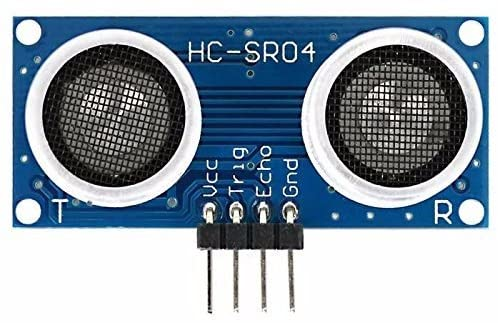
\includegraphics[width=.65\linewidth]{chapters/images/us.jpg} 
    \caption{Sensor ultrasonidos} 
  \end{minipage}%%
  \begin{minipage}[b]{0.5\linewidth}
    \centering
    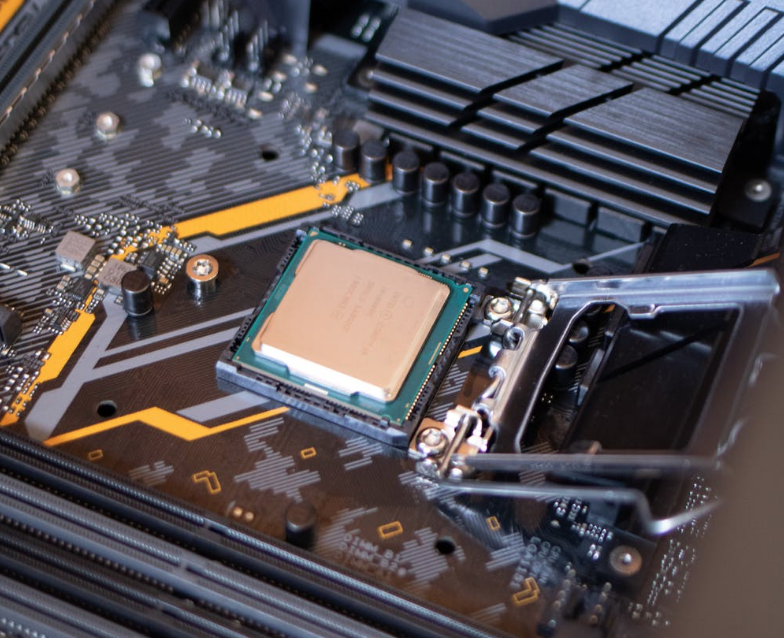
\includegraphics[width=.65\linewidth]{chapters/images/procesador.png} 
    \caption{Procesador} 
  \end{minipage} 
  \begin{minipage}[b]{0.5\linewidth}
    \centering
    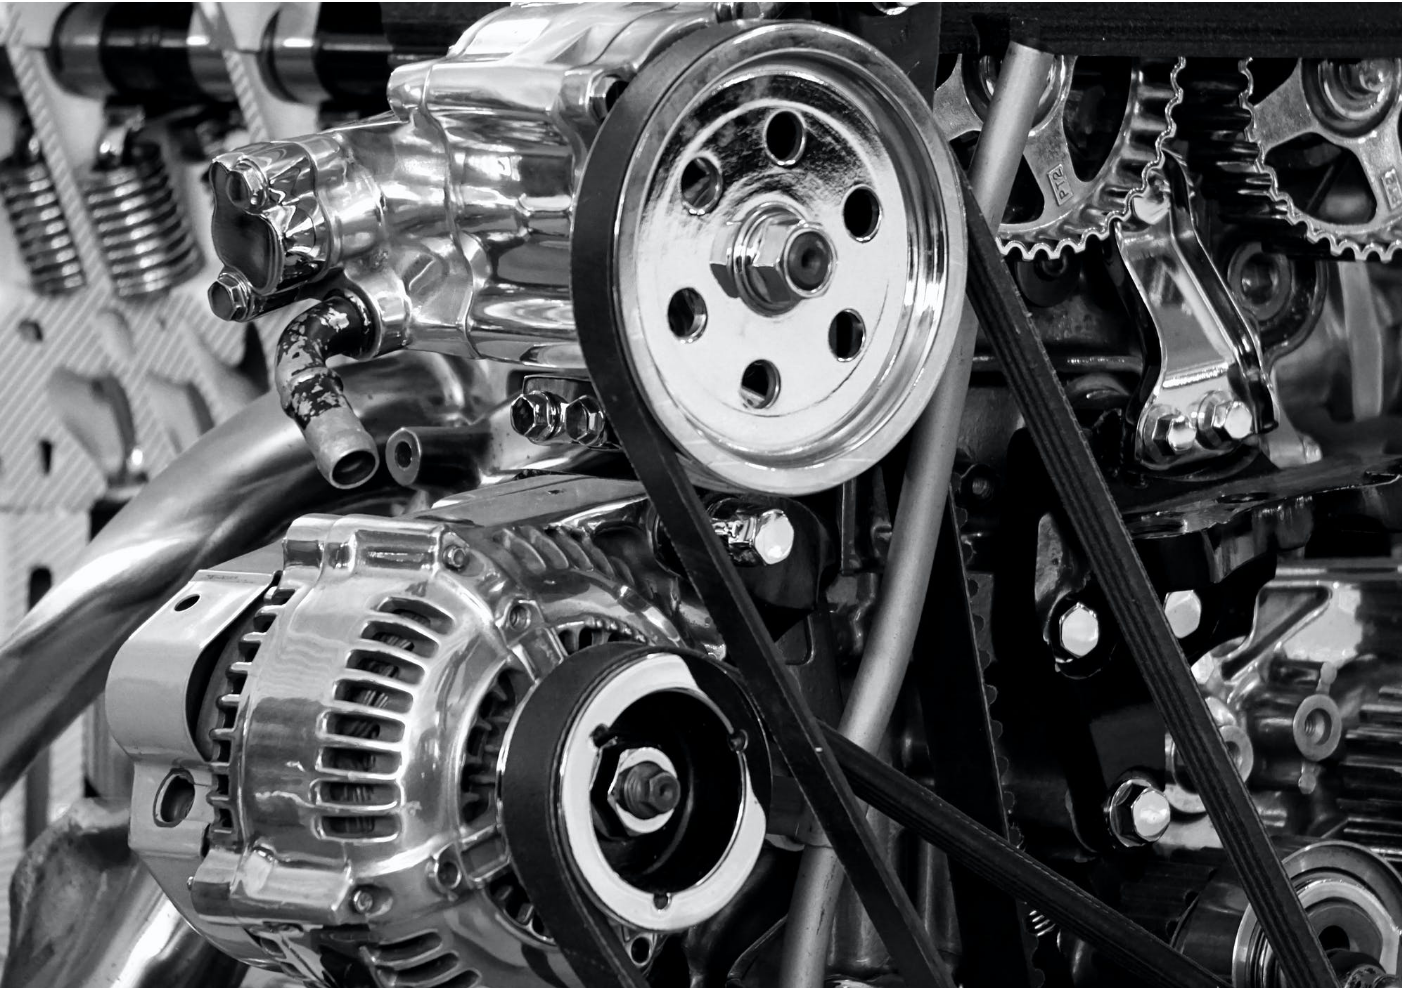
\includegraphics[width=.65\linewidth]{chapters/images/motor.png} 
    \caption{Servomotores} 
  \end{minipage}%% 
  \begin{minipage}[b]{0.5\linewidth}
    \centering
    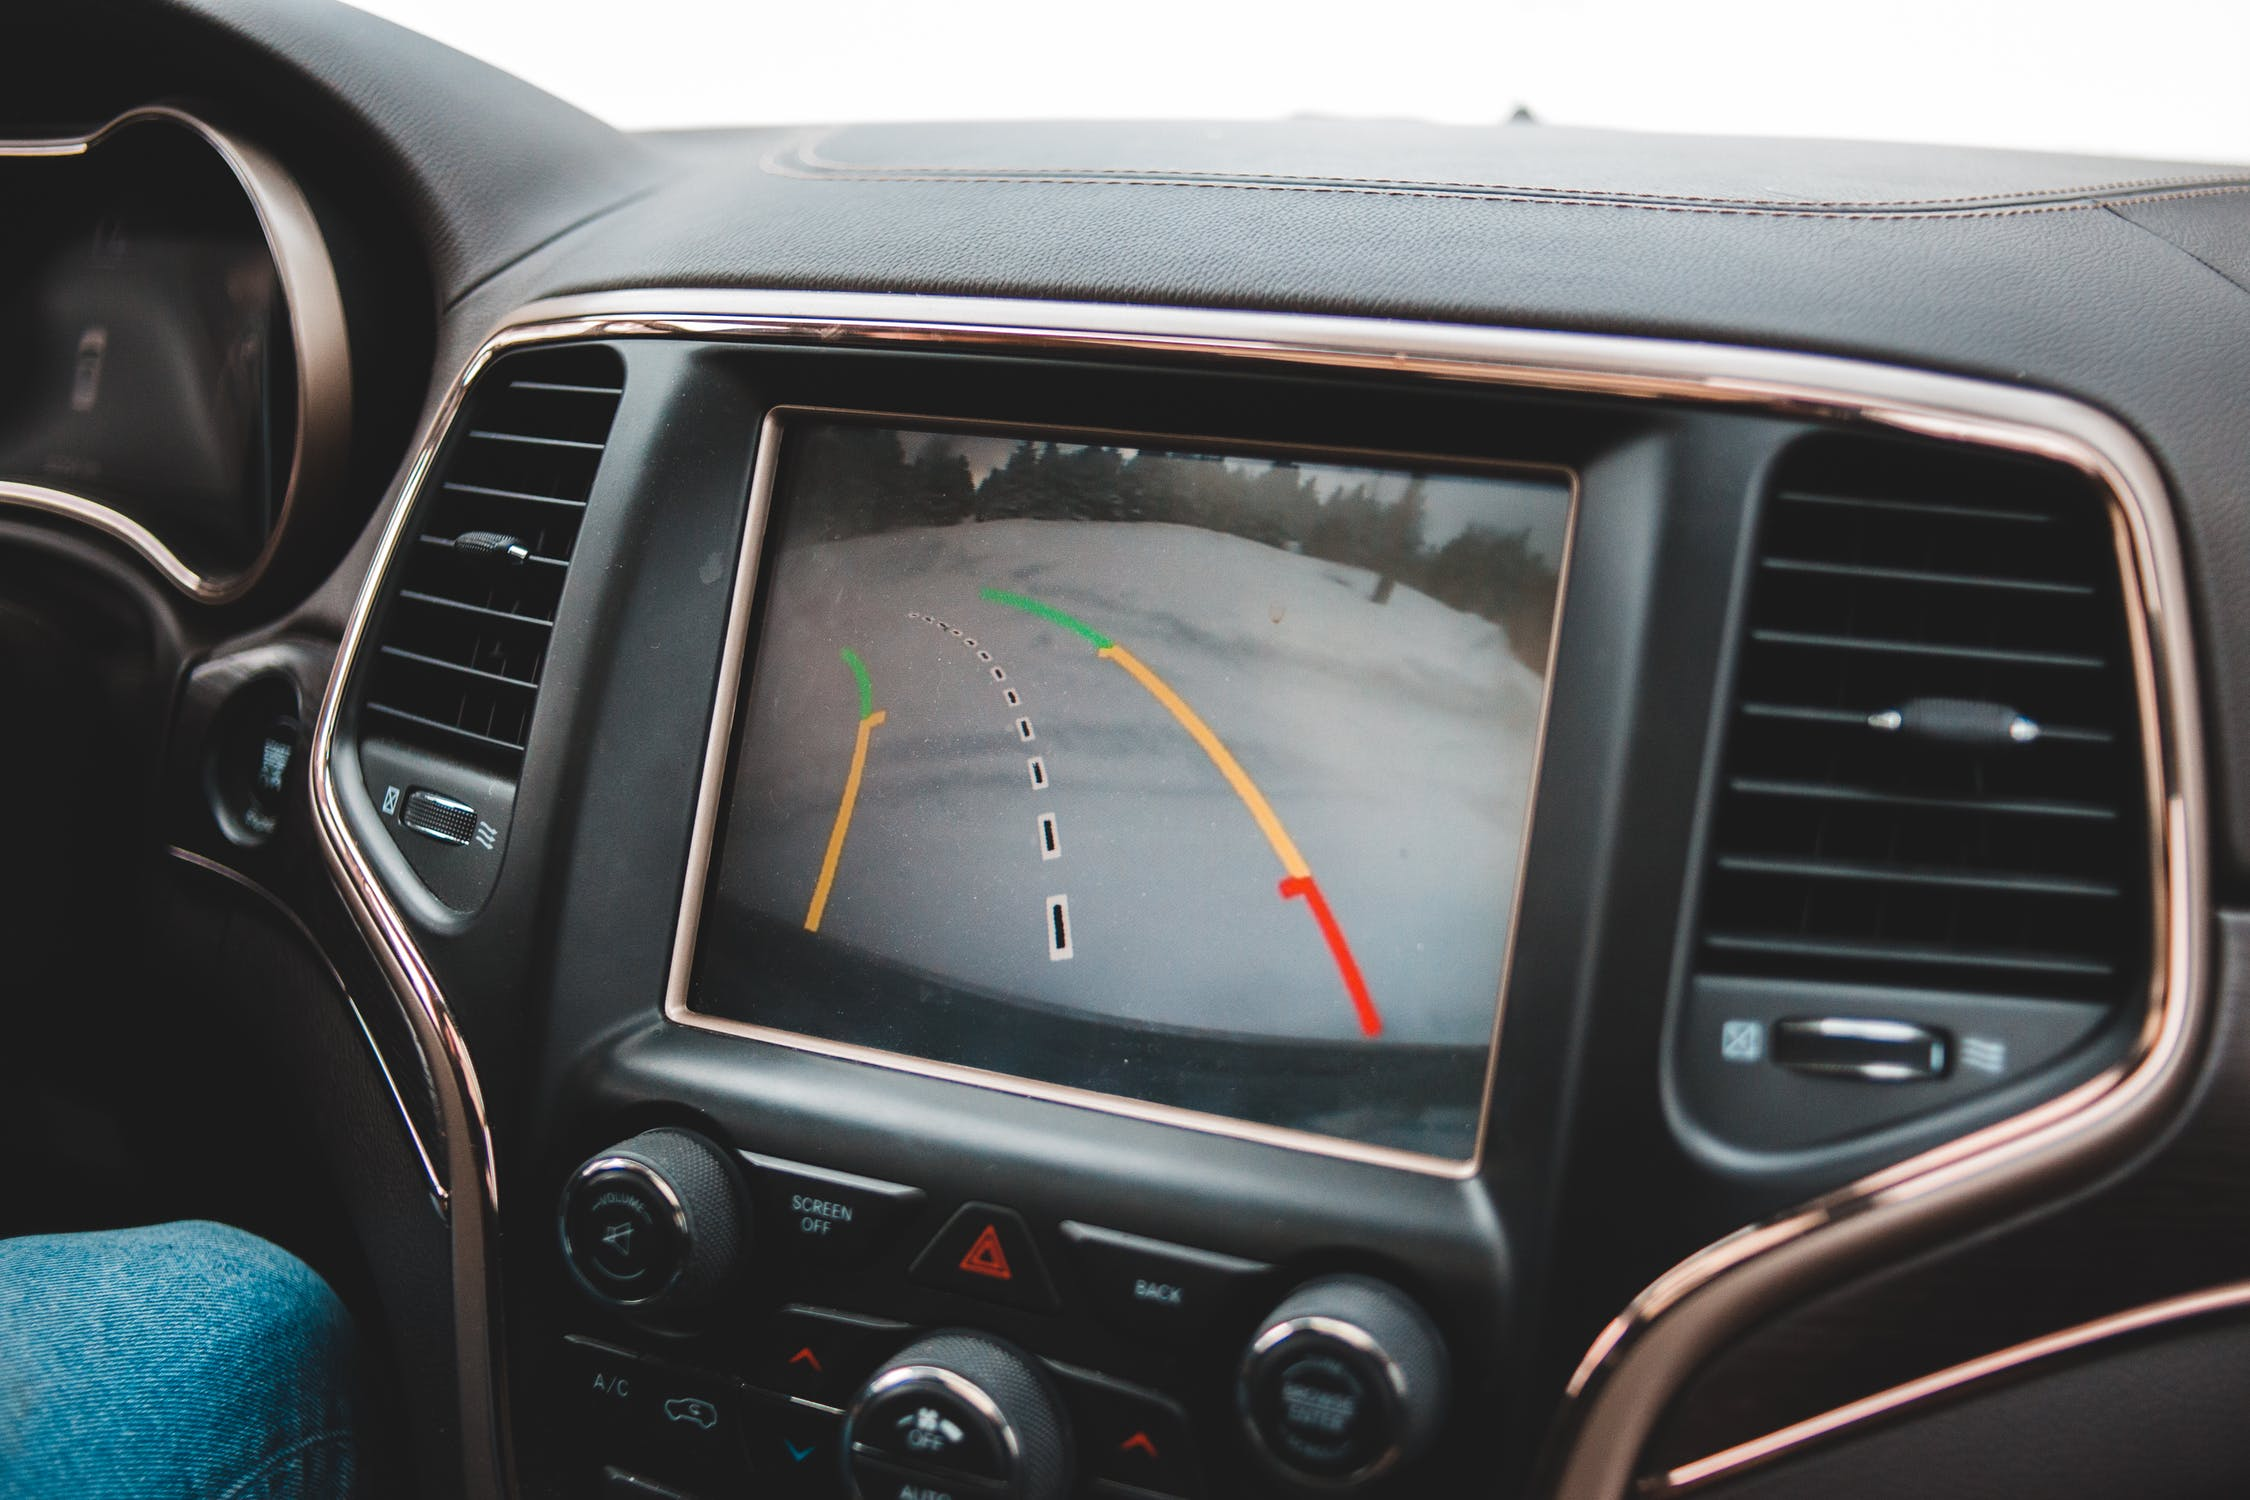
\includegraphics[width=.65\linewidth]{chapters/images/pantalla.jpeg} 
    \caption{Pantalla} 
  \end{minipage} 
\end{figure}

Los robots se clasifican según su entorno de aplicación en robots industriales y robots de servicio. También se pueden diferenciar según su forma en androides y zoomórficos, según su capacidad de movimiento en fijos o móviles, o según el medio en el que trabajan en terrestres, acuáticos o áereos. Estas son algunas de sus aplicaciones:
\begin{itemize}
    \item Robots industriales: brazos y pinzas robóticas para ensamblado de piezas, envasado de alimentos, industria automovilística y gestión de almacenes.
    \item Robots de servicio: destinados a limpieza del hogar, asistencia, coches autónomos, entrentenimiento, usos militares, limpieza de centrales nucleares, investigación en terrenos hostiles o fines médicos.
\end{itemize} 

 En la Figura 1.5 se muestran algunos ejemplos de robots que son de gran utilidad en la sociedad actual. 

\begin{figure}[H]
  \begin{subfigure}[b]{0.3\textwidth}
    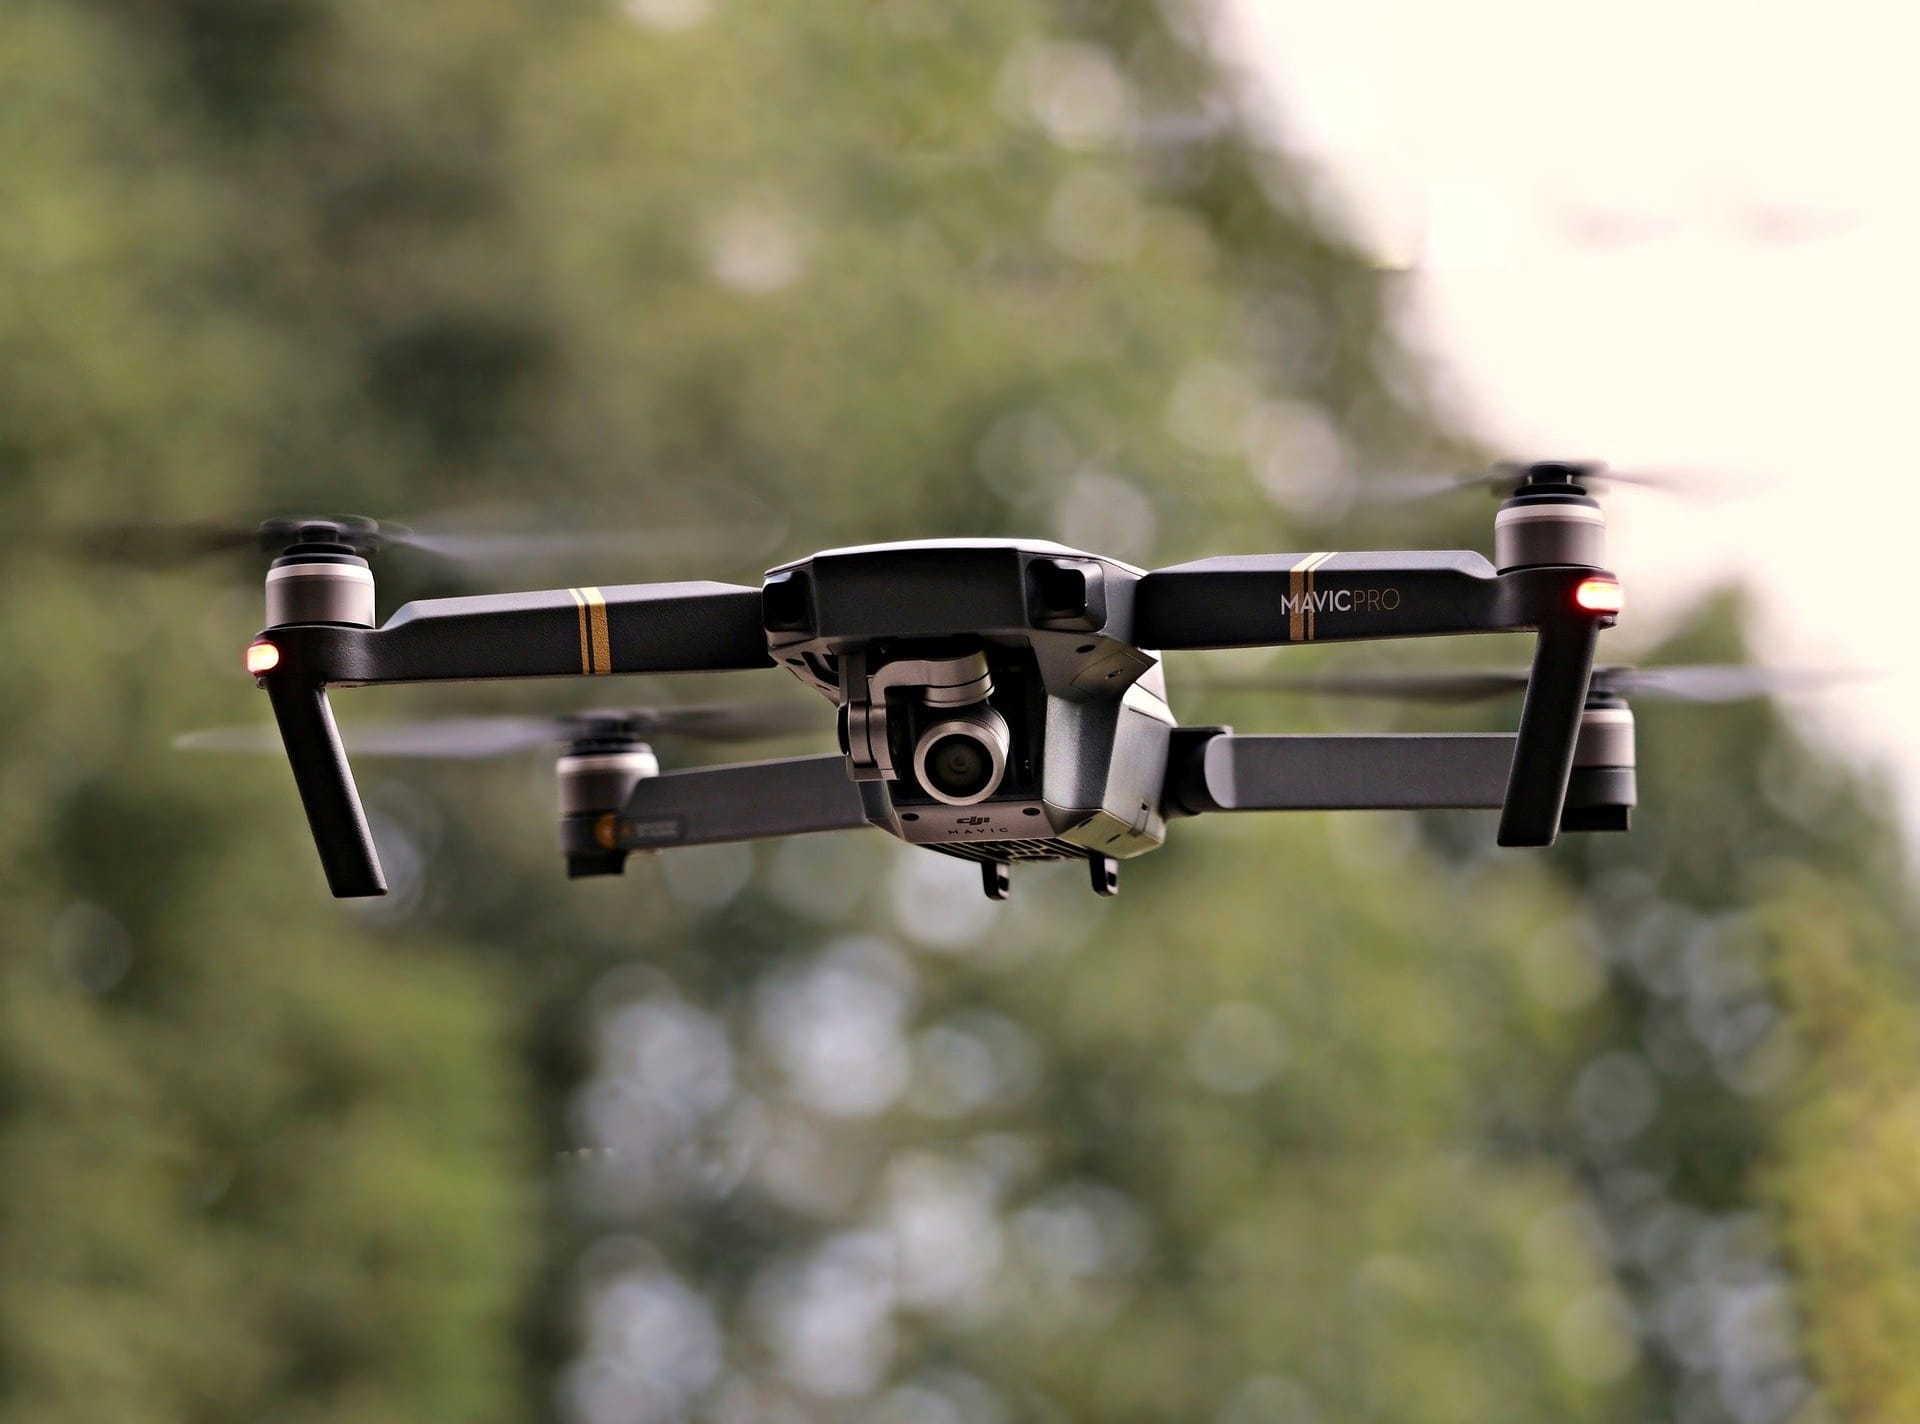
\includegraphics[width=\textwidth, height=\textwidth]{chapters/images/drone.jpeg}
    \caption{Dron}
    \label{fig:f1}
  \end{subfigure}
  \hfill
  \begin{subfigure}[b]{0.3\textwidth}
    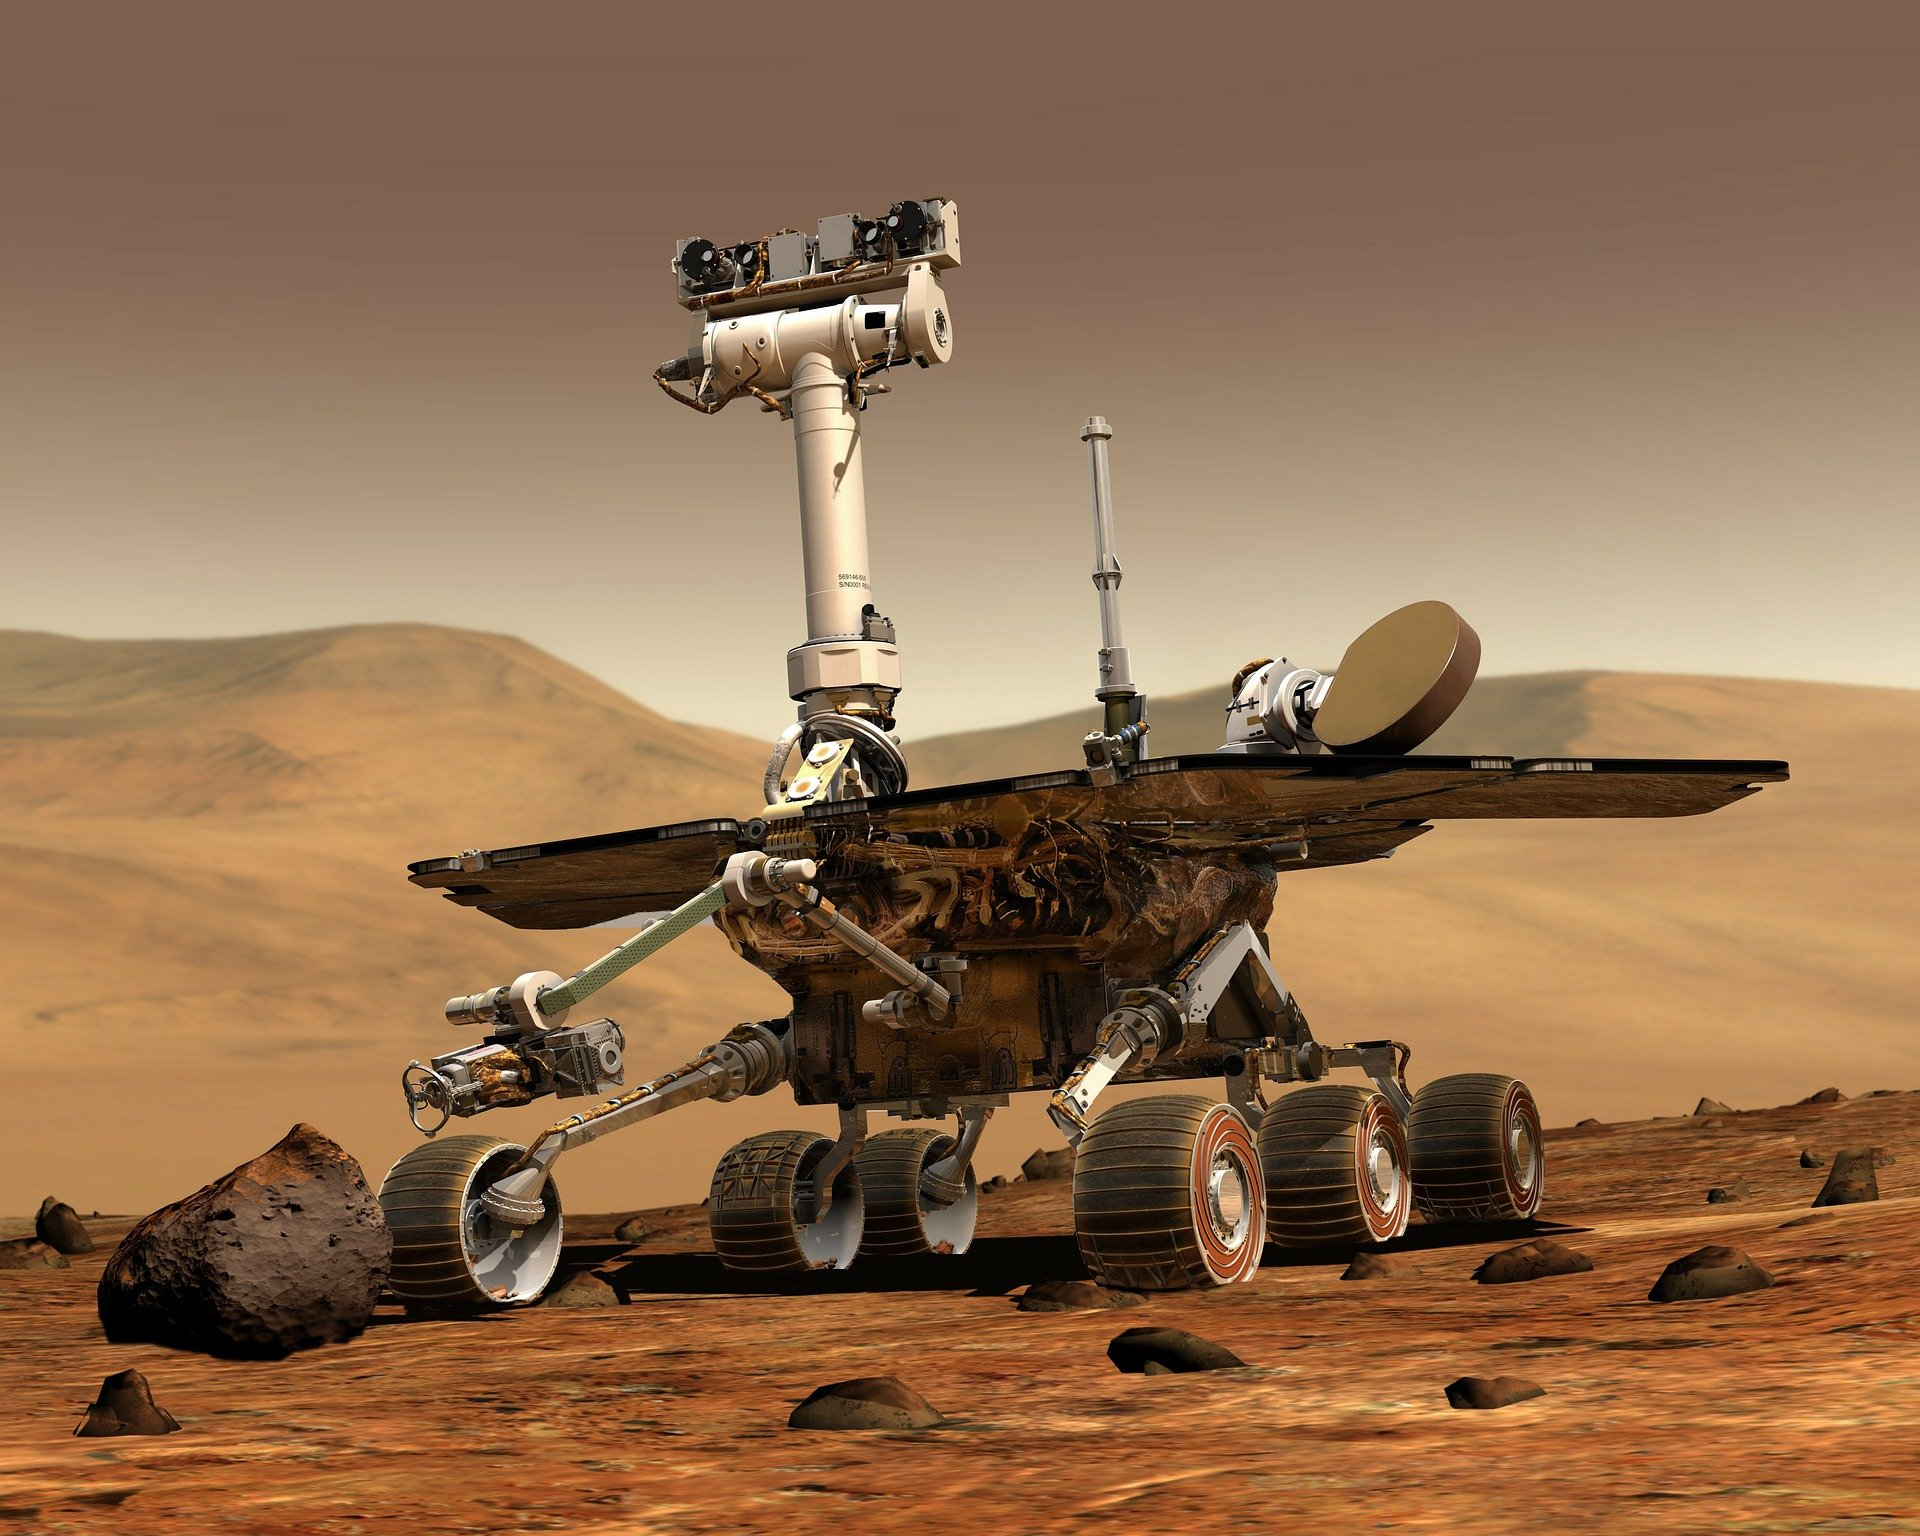
\includegraphics[width=\textwidth, height=\textwidth]{chapters/images/mars.jpg}
    \caption{Perseverance Mars}
    \label{fig:f2}
  \end{subfigure}
  \hfill
   \begin{subfigure}[b]{0.3\textwidth}
    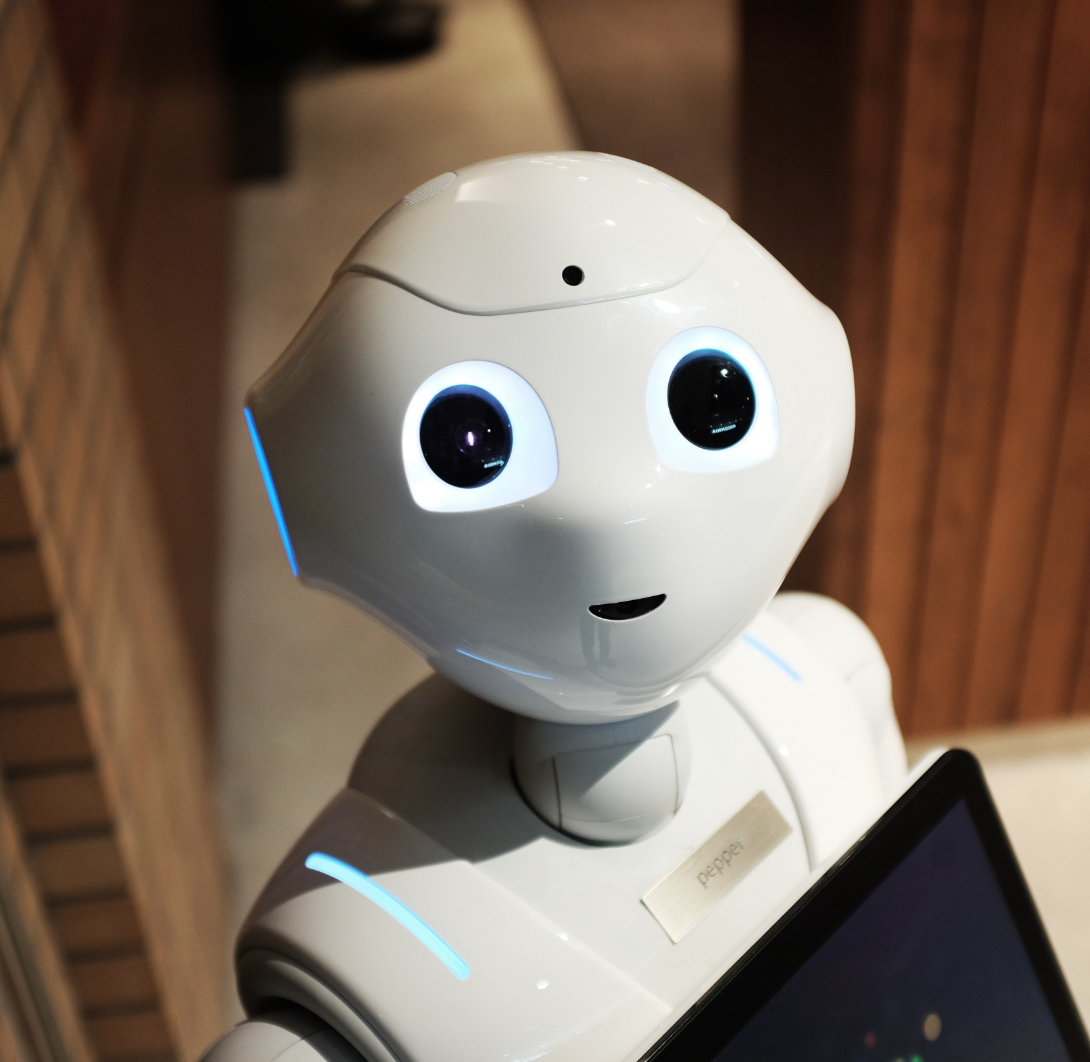
\includegraphics[width=\textwidth, height=\textwidth]{chapters/images/nao.png}
    \caption{Nao}
    \label{fig:f3}
  \end{subfigure}
  \hfill
   \begin{subfigure}[b]{0.3\textwidth}
    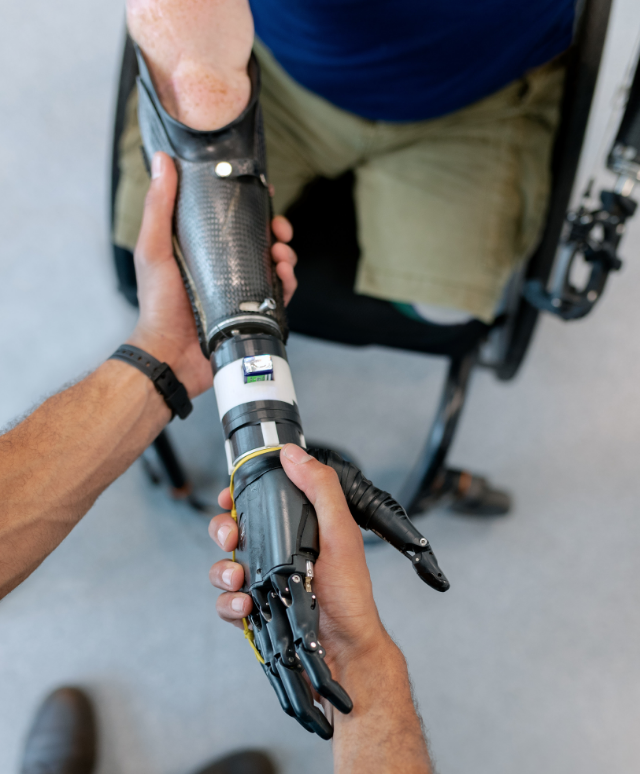
\includegraphics[width=\textwidth, height=\textwidth]{chapters/images/brazo.png}
    \caption{Brazo biónico}
    \label{fig:f4}
  \end{subfigure}
  \hfill
   \begin{subfigure}[b]{0.3\textwidth}
    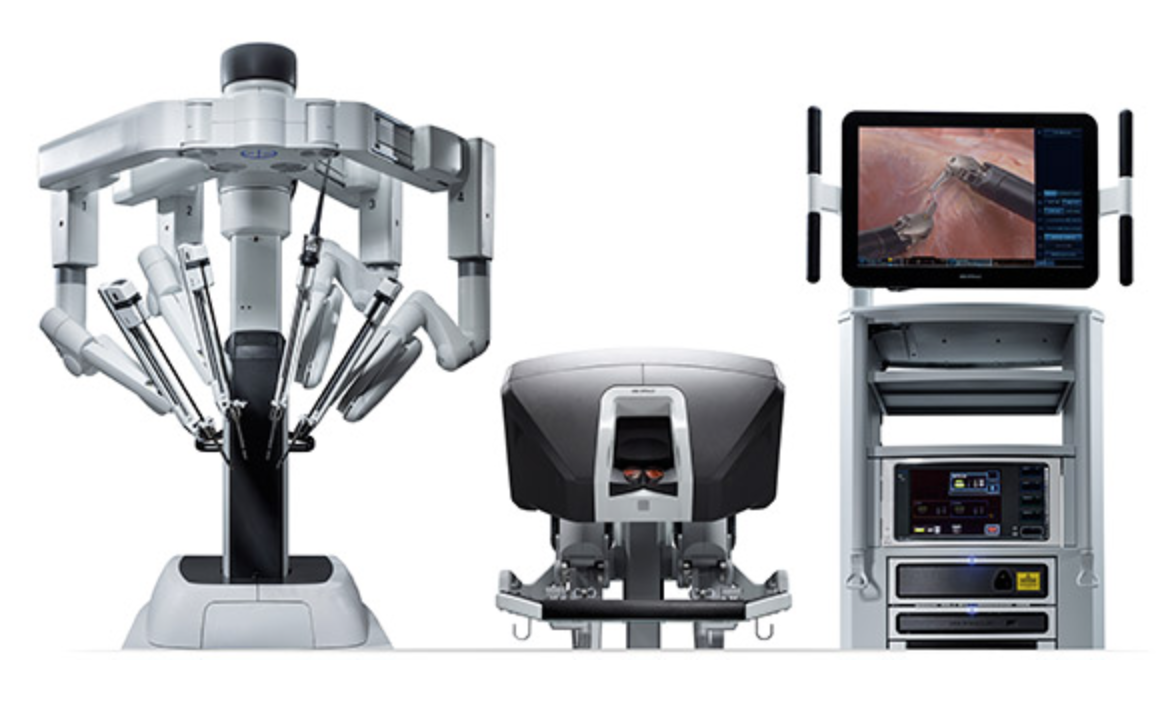
\includegraphics[width=\textwidth, height=\textwidth]{chapters/images/davinci.png}
    \caption{Da Vinci \cite{davinci} }
    \label{fig:f5}
  \end{subfigure}
  \hfill
   \begin{subfigure}[b]{0.3\textwidth}
    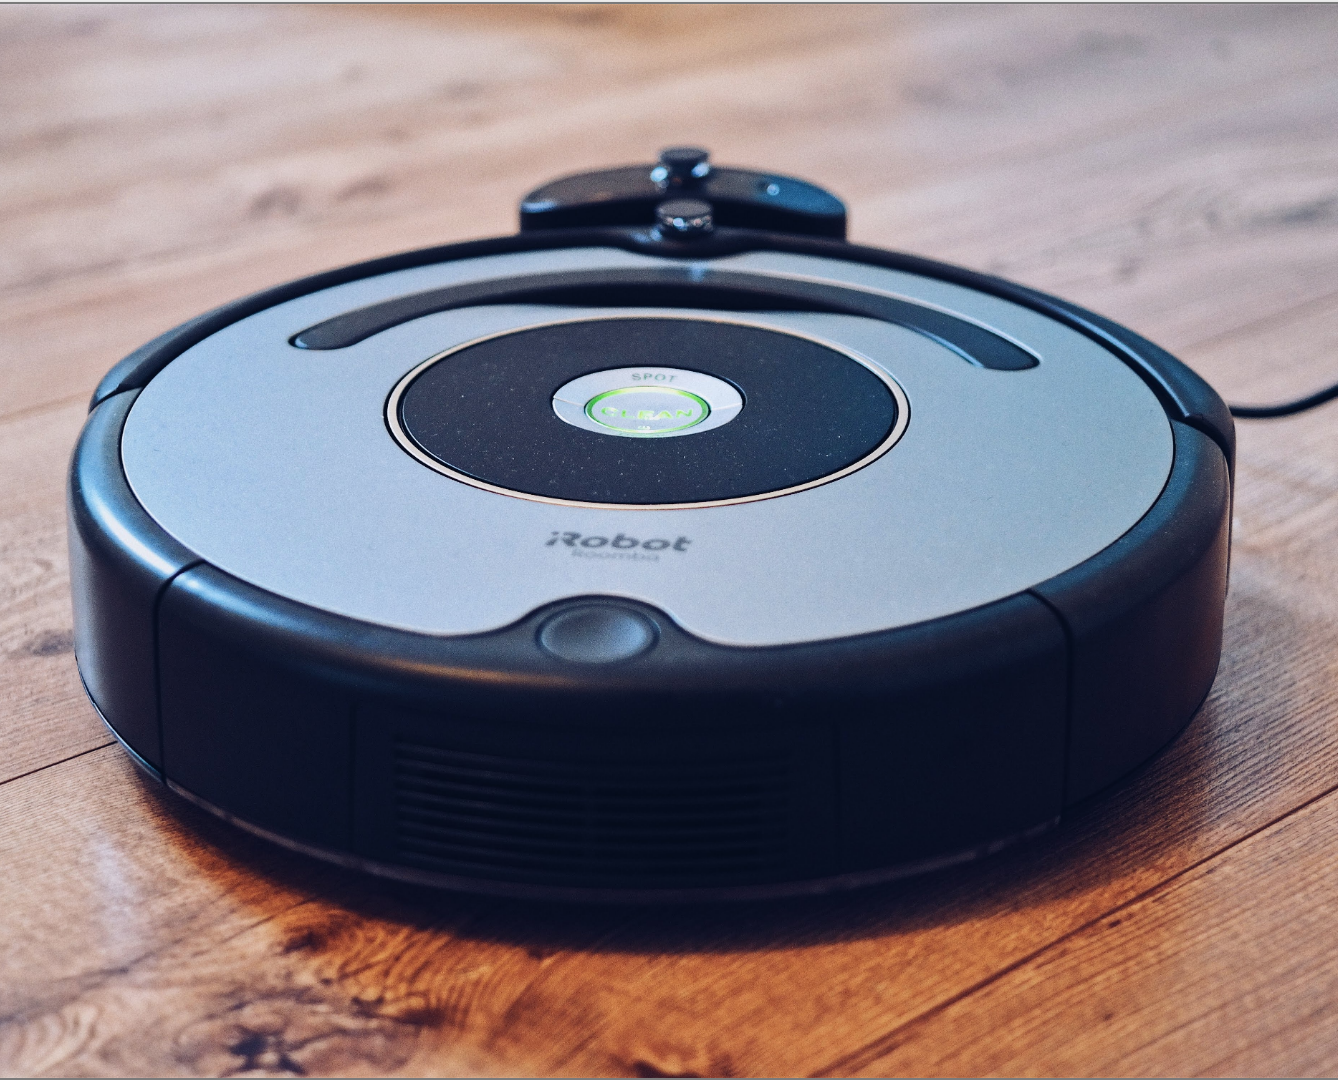
\includegraphics[width=\textwidth, height=\textwidth]{chapters/images/roomba.png}
    \caption{Roomba}
    \label{fig:f6}
  \end{subfigure}
  \caption{Ejemplos de Robots}
\end{figure}

La Figura 1.5(a) muestra un dron, estos pequeños vehículos no tripulados han sido toda una revolución en la grabación de eventos y películas. El entretenimiento no es su única aplicación, también se utilizan para la búsqueda de personas y vigilancia. 

El Perseverance Mars que vemos en la Figura 1.5(b) actualmente está en Marte haciendo investigaciones del terreno. Este robot busca signos de vida y guarda muestras para un futuro regreso a la Tierra.

Los robots de asistencia como el Nao, Figura 1.5 (c), son muy importantes para que los más pequeños y las personas mayores puedan socializar de una forma divertida y a su vez es una herramienta de apoyo en procesos de rehabilitación, post-operatorios y terapias ocupacionales.

Los brazos biónicos como el de la Figura 1.5(d) permiten recuperar las funciones y el tacto a amputados. El robot Da Vinci Figura 1.5(e) ayuda a los cirujanos a operar con mayor precisión y seguridad.  Estos robots han sido un gran avanze en el campo de la medicina.

El robot aspirador, uno del más conocido es \textit{Roomba}, Figura 1.5(f), es capaz de detectar obstáculos y residuos en el suelo. Esto nos ayuda a que la casa esté limpia y nos ahorra mucho tiempo.

Los robots que se han mencionado son solo algunos ejemplos. La robótica es una tecnología en auge. En los últimos años, con el avance de la tecnología, la realidad ha superado a la ficción, estamos rodeados de robots. Han salido de los laboratorios y han surgido miles de aplicaciones que nos hacen la vida un poco mejor.
\\
\\

Recientemente la robótica se está incorporando también a las aulas para que los más pequeños adquieran conocimientos y habilidades importantes para su futuro. En la siguiente Figura 1.6 se muestran unos ejemplos de robots diseñados para el ámbito educativo. \cite{roboticakids}

\begin{figure}[H]
    \centering
    \begin{subfigure}{.3\linewidth}
        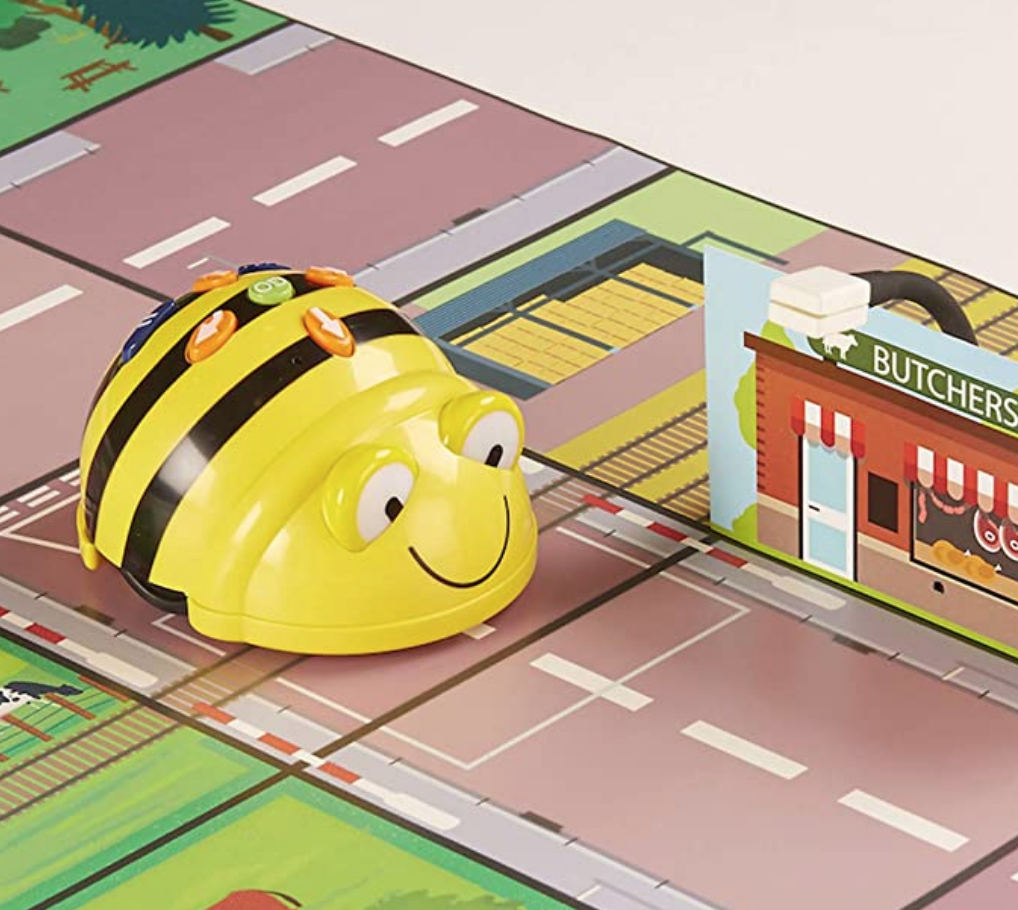
\includegraphics[width=1\textwidth]{chapters/images/beebot.png}
        \caption{Bee-bot}
    \end{subfigure}
    \hskip2em
    \begin{subfigure}{.3\linewidth}
    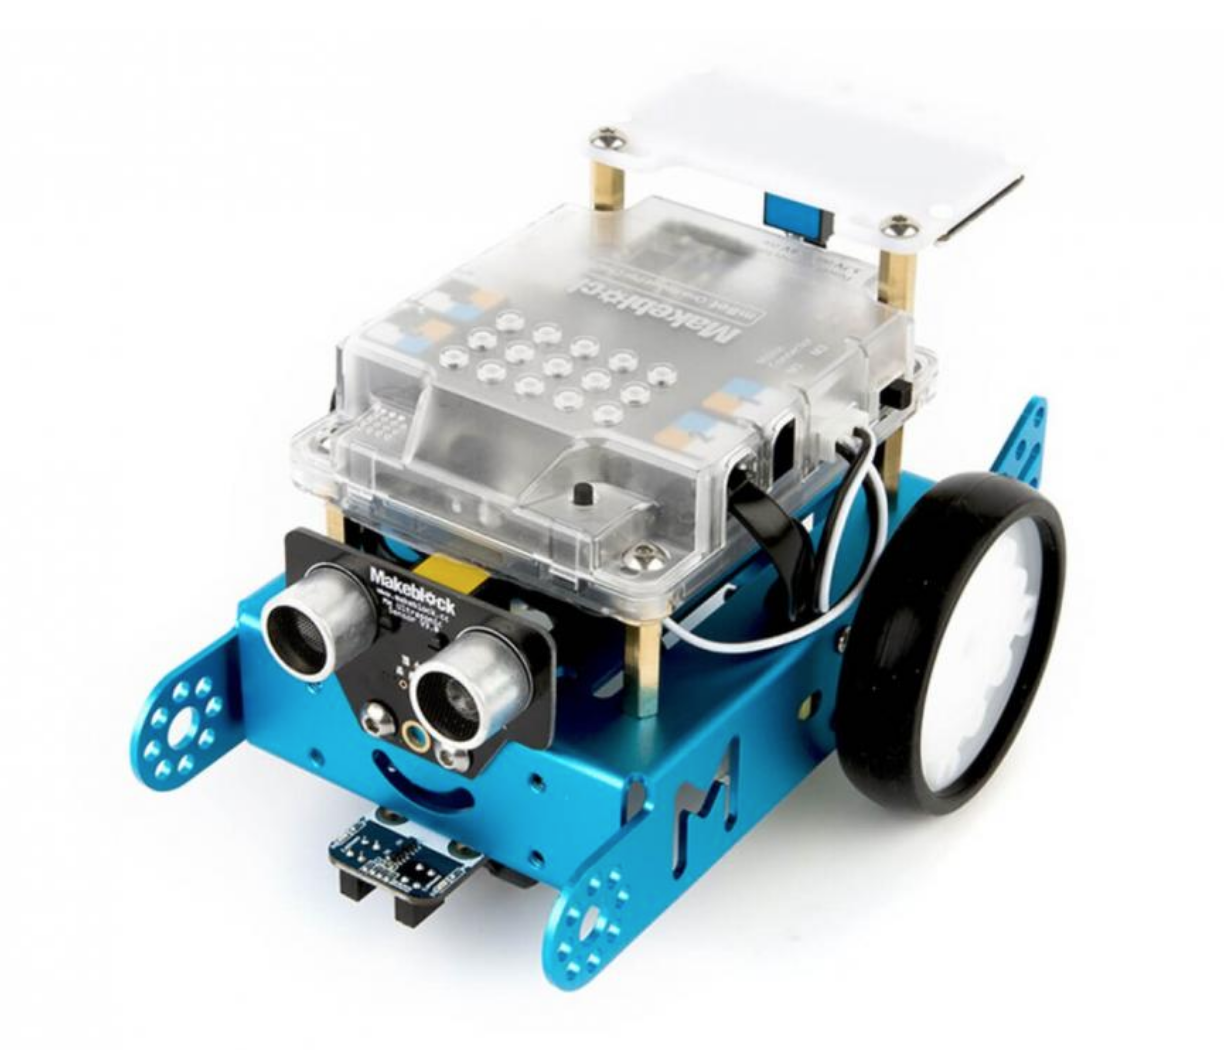
\includegraphics[width=1\textwidth]{chapters/images/mbot.png}
        \caption{Makeblock Mbot}
    \end{subfigure}
    \begin{subfigure}{.3\linewidth}
       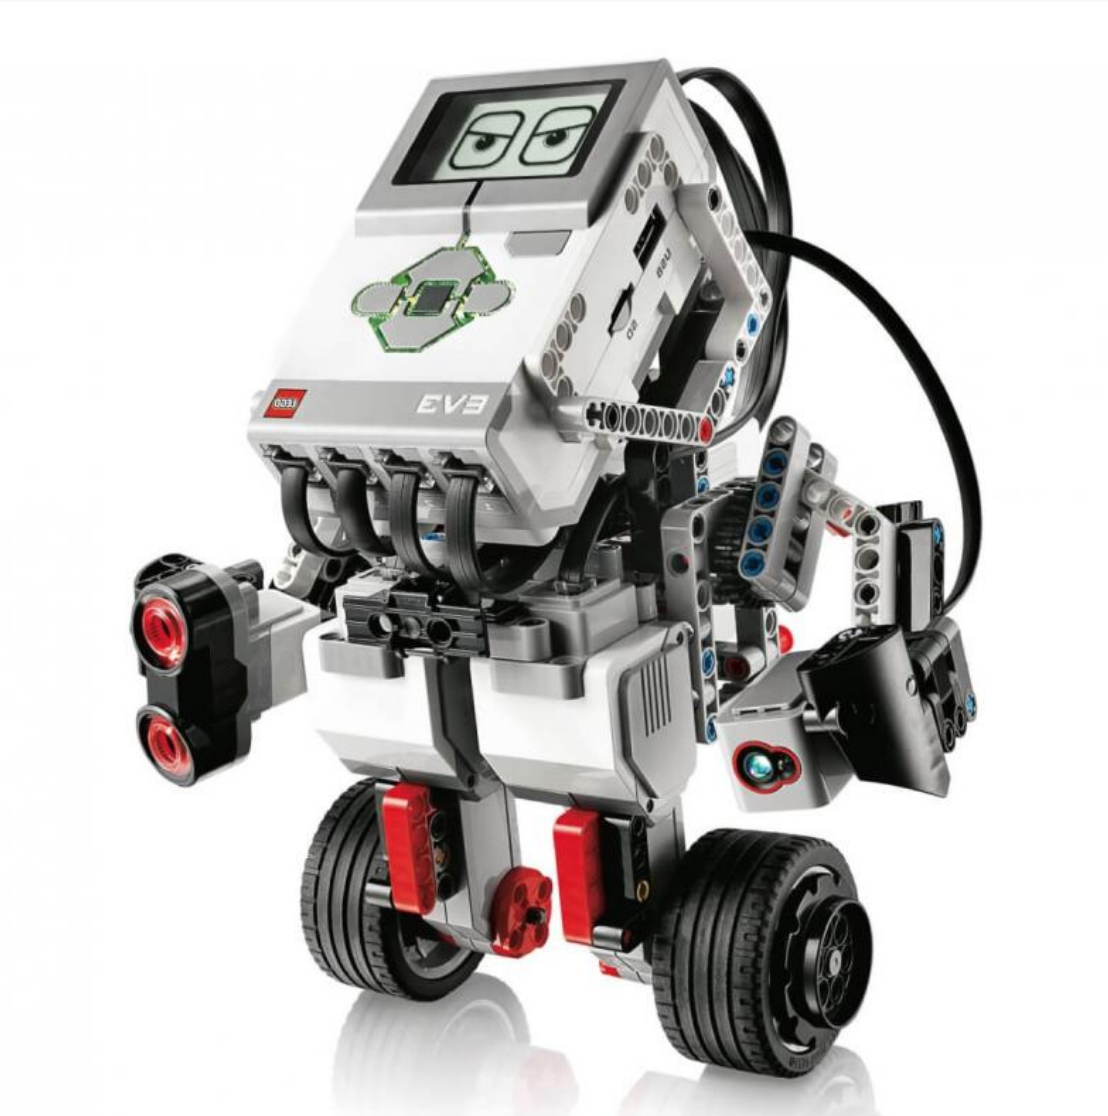
\includegraphics[width=1\textwidth]{chapters/images/lego.png}
        \caption{LEGO MINDSTORMS EV3}
    \end{subfigure}
    \caption{Ejemplos de Robots educativos}
\end{figure}


%%%%%%%%%%%%%%%%%%%%%%%%%
\newpage
\section{Tecnologías Web}
Las tecnologías web juegan un papel muy importante en el mundo moderno gracias a Internet. Esta plataforma WWW \footnote{World Wide Web}\cite{www}
ha ido evolucionando y ha posibilitado potentes aplicaciones con un modelo cliente/servidor. En la Figura 1.7 podemos ver algunos ejemplos de aplicaciones web.

\begin{figure}[H]
\begin{subfigure}{.5\textwidth}
  \centering
  % include first image
  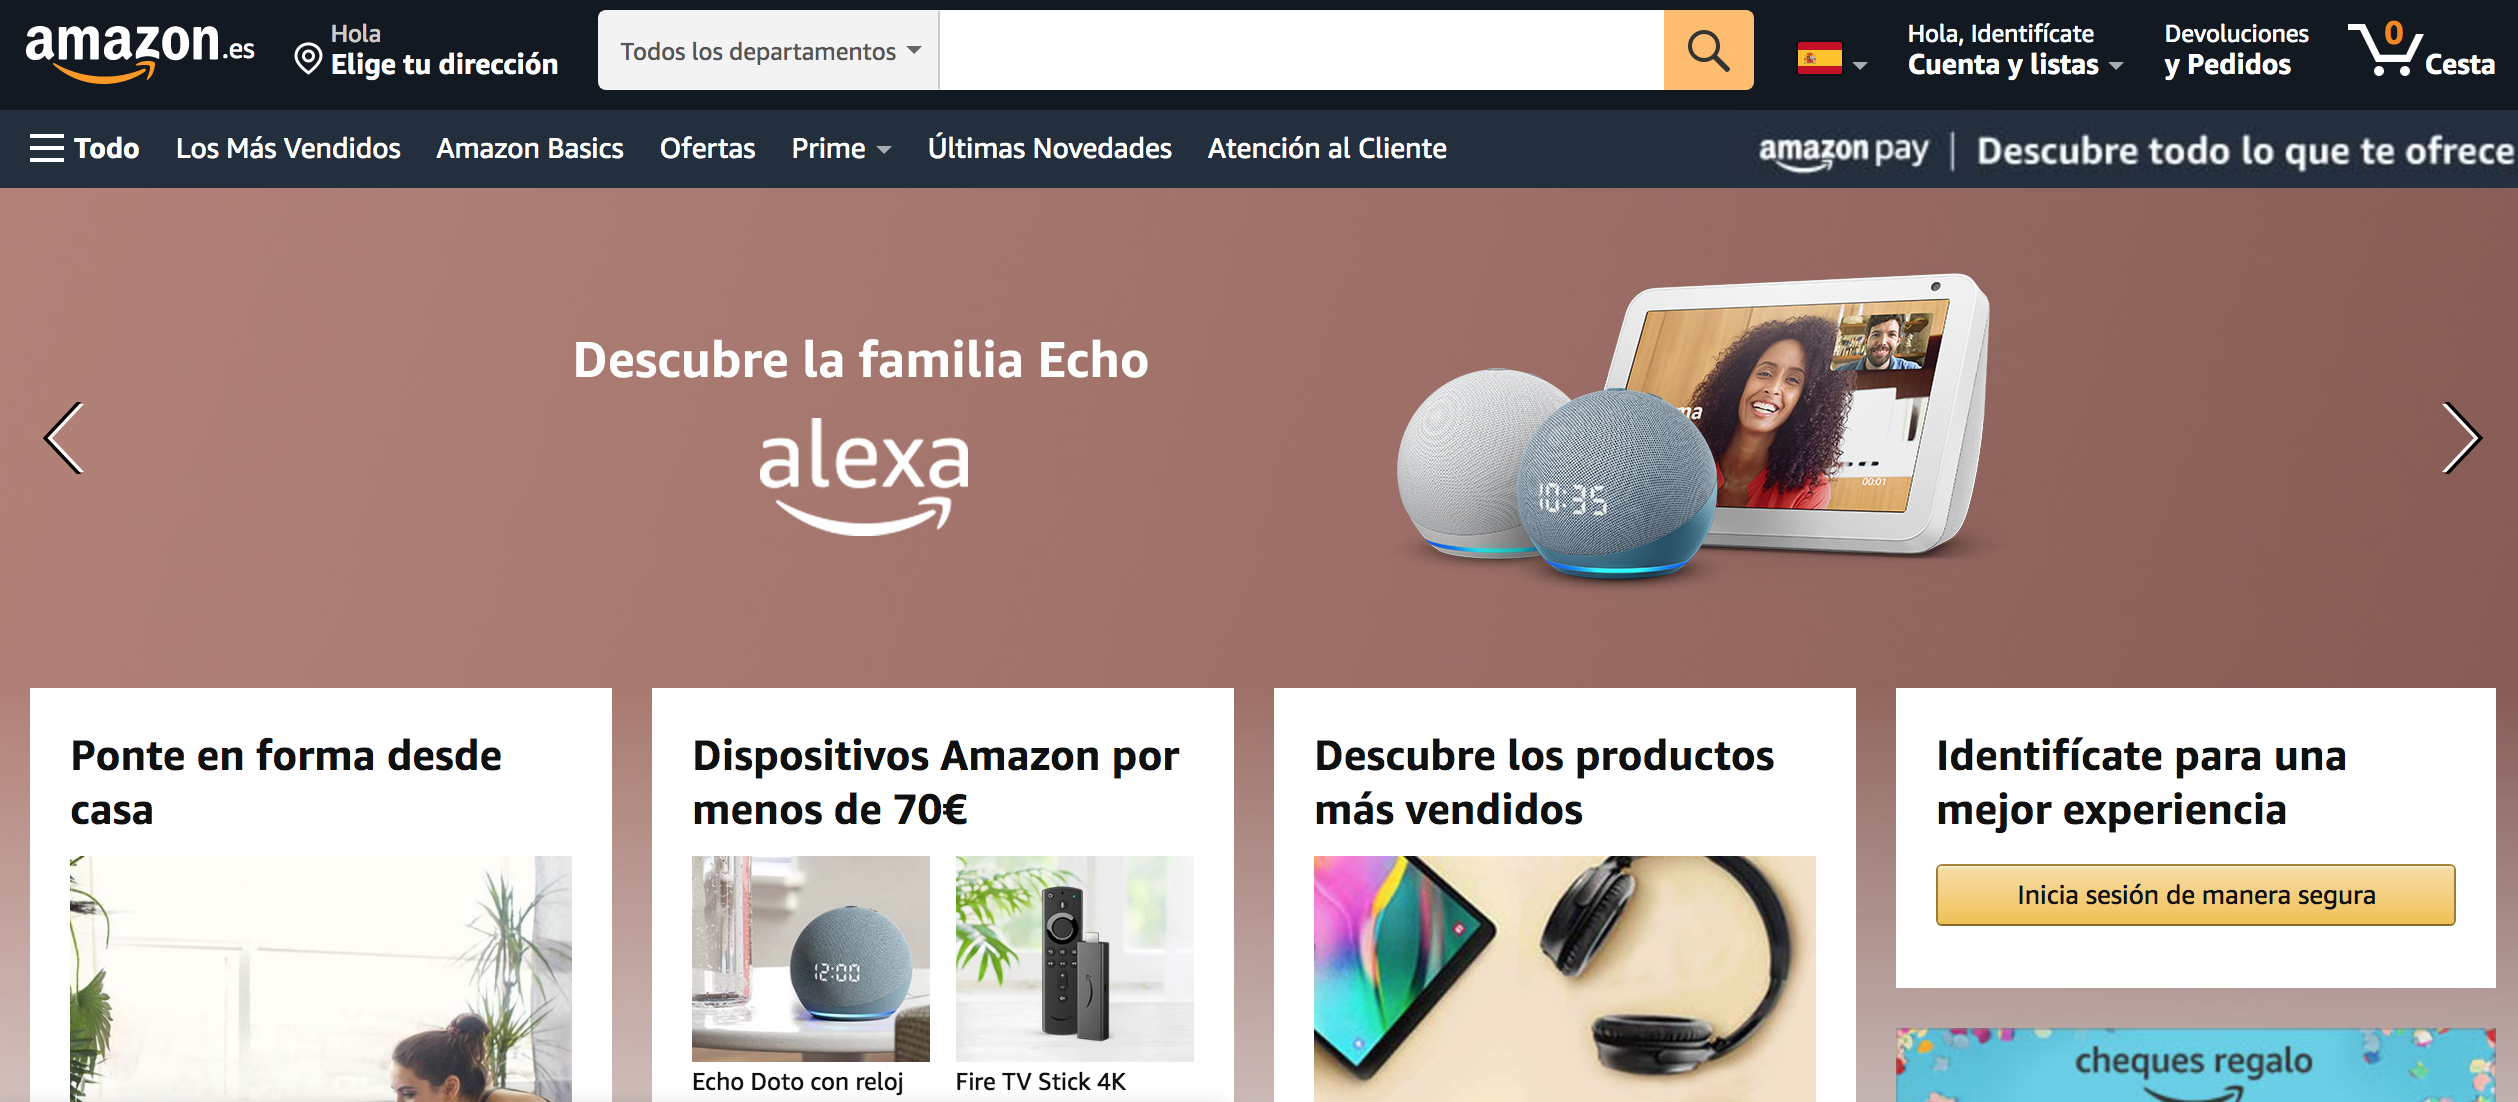
\includegraphics[width=.8\linewidth]{chapters/images/amazon.png}
  \caption{Amazon}
  \label{fig:sub-first}
\end{subfigure}
\begin{subfigure}{.5\textwidth}
  \centering
  % include second image
  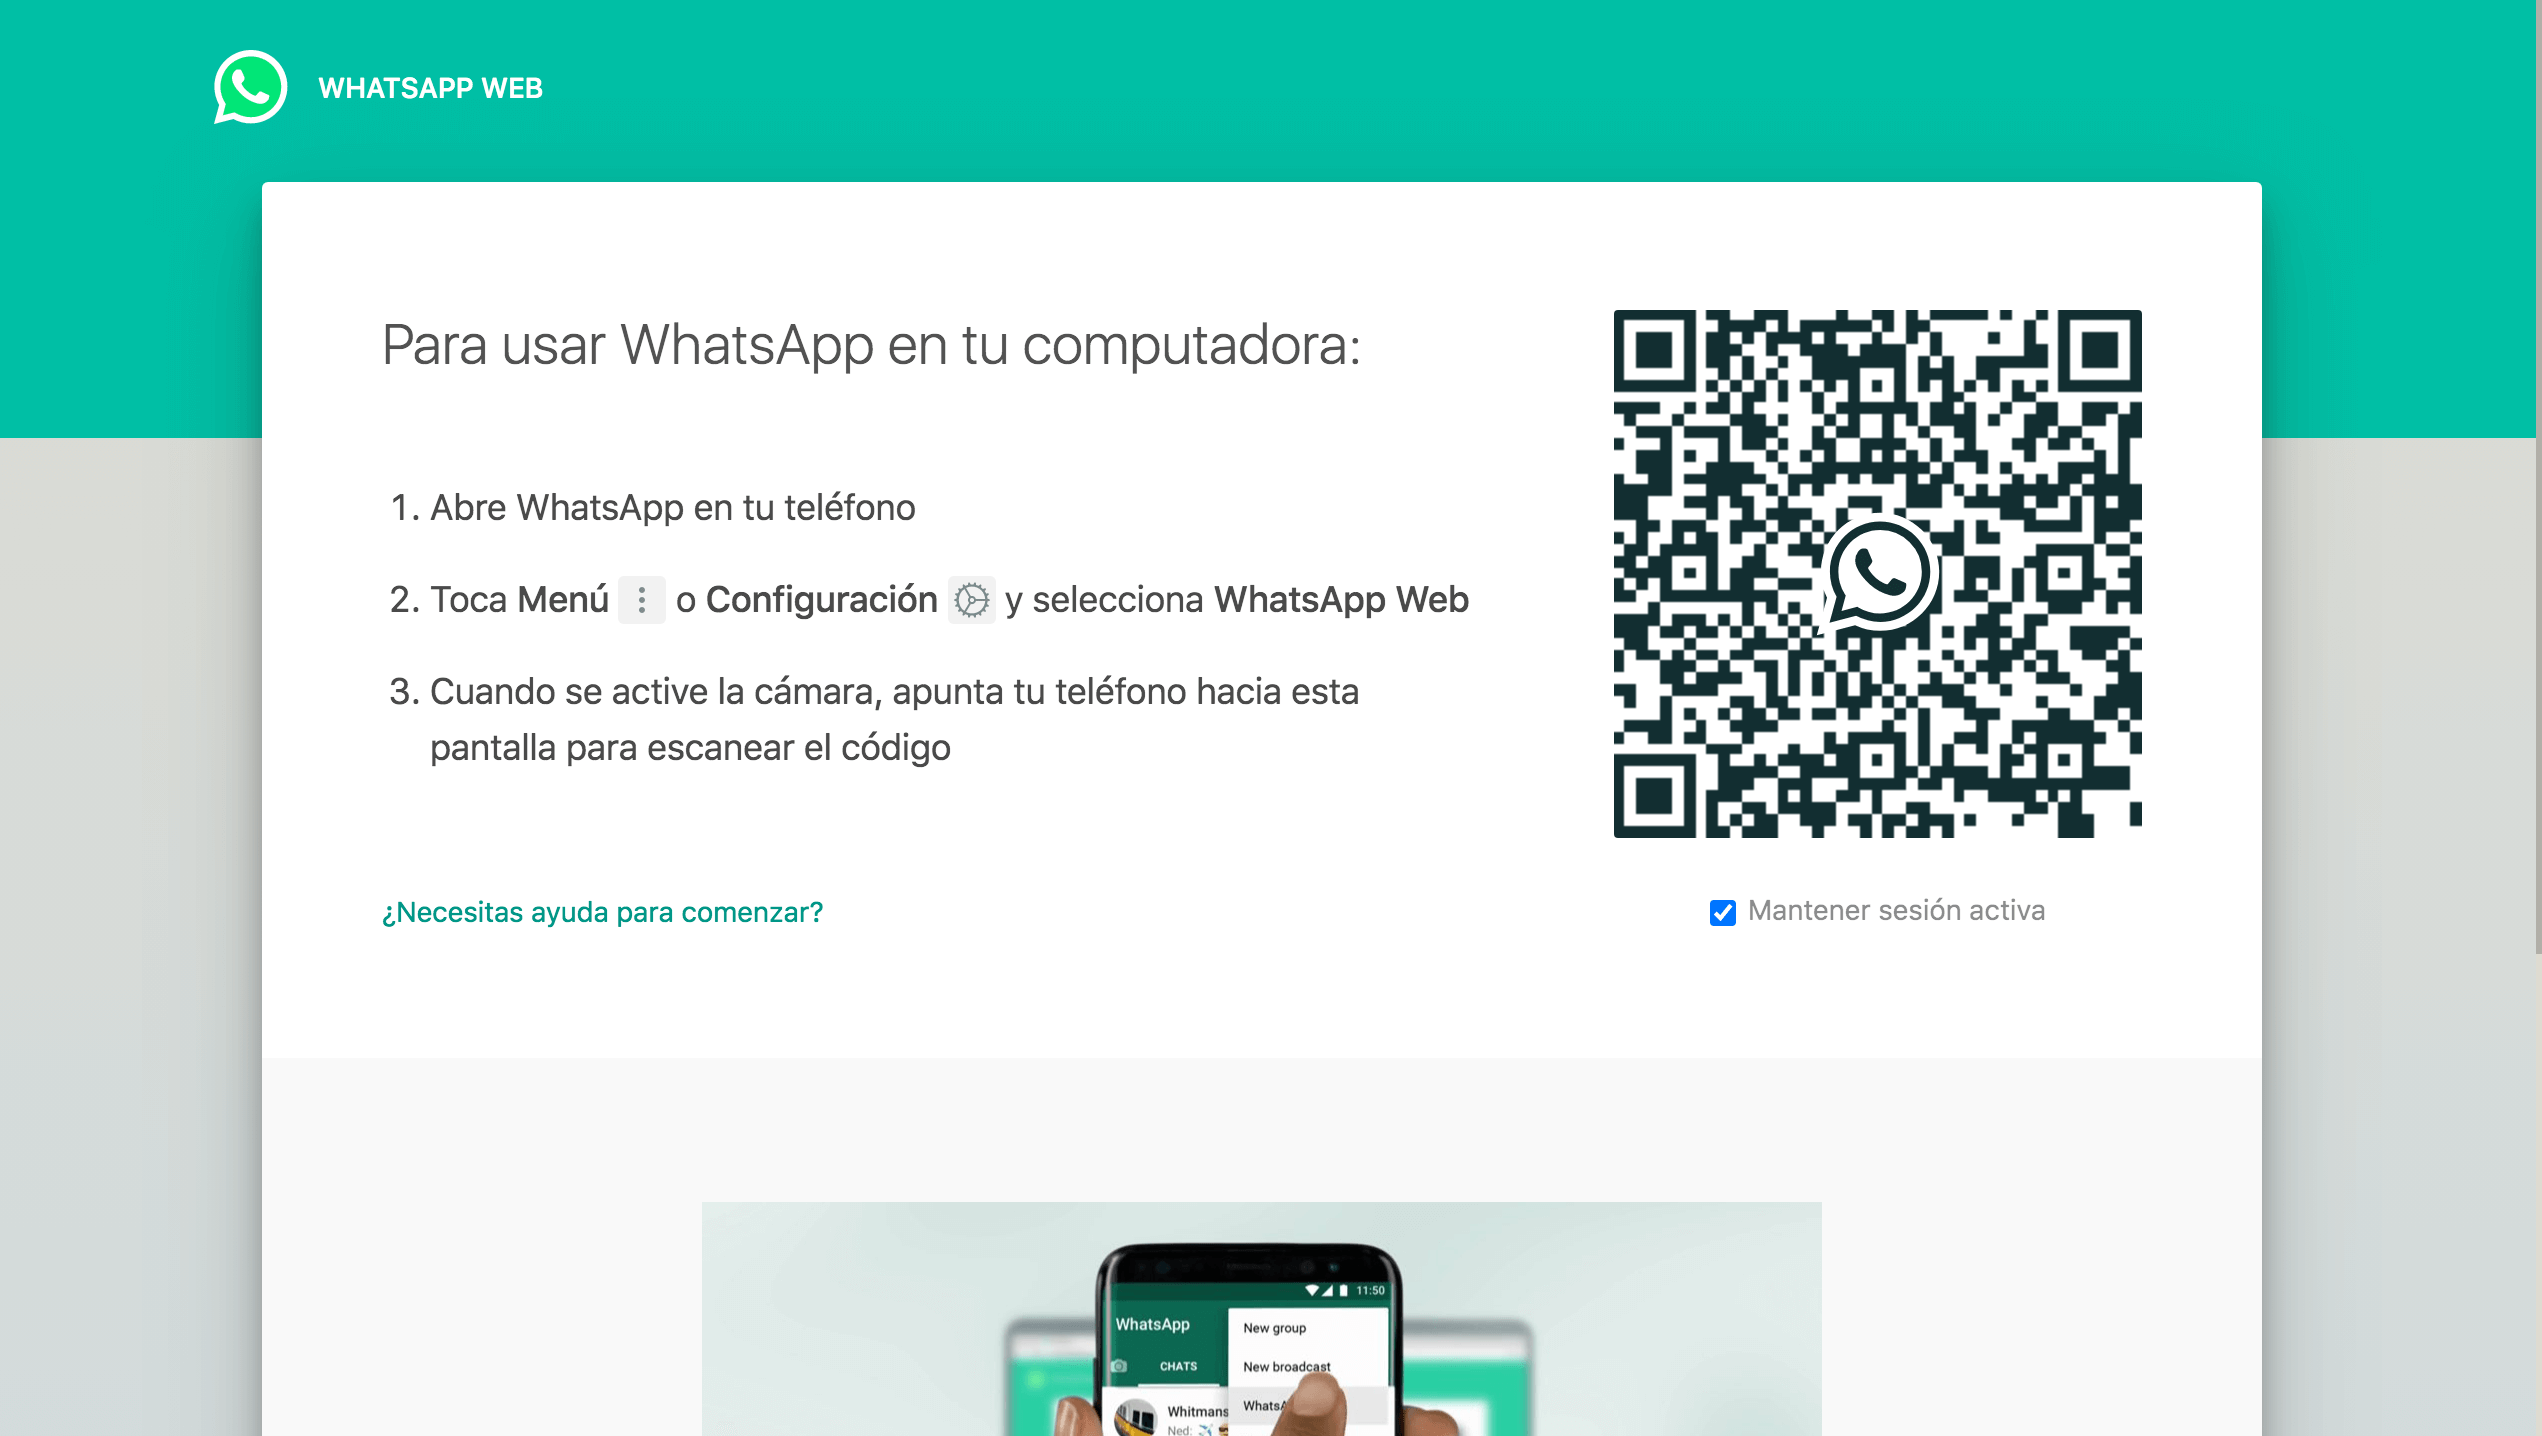
\includegraphics[width=.8\linewidth]{chapters/images/whatsappweb.png}  
  \caption{Whatsapp Web}
  \label{fig:sub-second}
\end{subfigure}
\begin{subfigure}{.5\textwidth}
  \centering
  % include third image
  
\includegraphics[width=.8\linewidth]{chapters/images/disney.jpeg}  
  \caption{Disney+}
  \label{fig:sub-third}
\end{subfigure}
\begin{subfigure}{.5\textwidth}
  \centering
  % include fourth image
  
\includegraphics[width=.8\linewidth]{chapters/images/urjcweb.png}  
  \caption{URJC}
  \label{fig:sub-fourth}
\end{subfigure}
\caption{Ejemplos aplicaciones web}
\label{fig:partes robot}
\end{figure}

La web es una colección de documentos enlazados a través de hiperenlaces, cada recurso queda definido por su URL \footnote{Uniform Resource Locator}. Cuando accedemos a la web a través del navegador, tenemos que introducir la dirección URL del sitio web al que nos queremos dirigir. El navegador enviará una solicitud al servidor con el protocolo HTTP \footnote{Hyper Text Transfer Protocol}. El servidor le enviará a nuestro navegador un fichero HTML que quedará almacenado en nuestra máquina. Una vez el navegador obtiene el fichero HTML mostrará al usuario la página web principal de la URL que ha introducido. Si el navegador detecta que hay imágenes, vídeos u otros ficheros, volverá a mandar peticiones HTTP al servidor para que éste le envíe toda la información necesaria. En la Figura 1.8 podemos ver una representación de cómo es la comunicación entre cliente y servidor.
\begin{figure}[H]
    \centering
    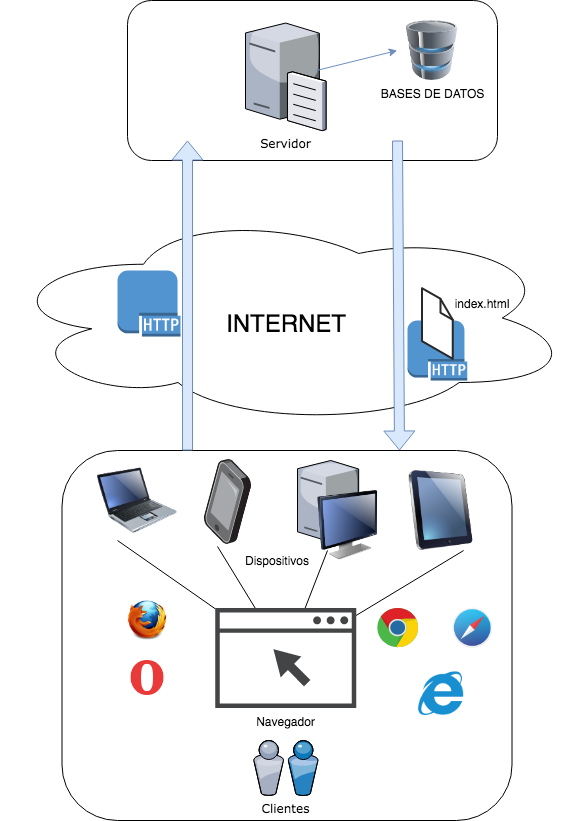
\includegraphics[width=0.45\columnwidth]{chapters/images/web.png}
    \caption{Comunicación cliente/servidor a través de HTTP}
    \label{fig:httpprotocol}
\end{figure}
 HTTP es un protocolo entre navegadores y servidores web para transferir documentos de hipertexto. El cliente envía mensajes de solicitud y el servidor manda mensajes de respuesta, ambos mensajes son del mismo formato (ver Figura 1.9 y Figura 1.10.) Los tipos de mensaje más comunes de este protocolo son GET, POST, PUT, DELETE y HEAD. Este protocolo utiliza códigos de estado, los más conocidos son: 200 OK, que significa resultado exitoso, 500 Server Error, cuando hay un error en el lado servidor y el más conocido 404 Not Found, cuando hay un error en la parte cliente. \cite{tecnologiasweb}

\begin{figure}[H]
\centering
\begin{minipage}[t]{.45\linewidth}
\centering
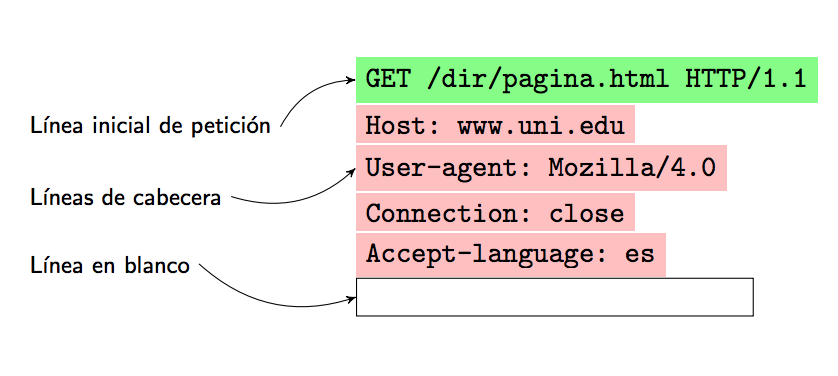
\includegraphics[width=1\columnwidth]{chapters/images/peticionhttp.png}
\caption{Ejemplo petición HTTP\\ Cliente a Servidor}
\end{minipage}
\hspace{0.25in}
\begin{minipage}[t]{.45\linewidth}
\centering
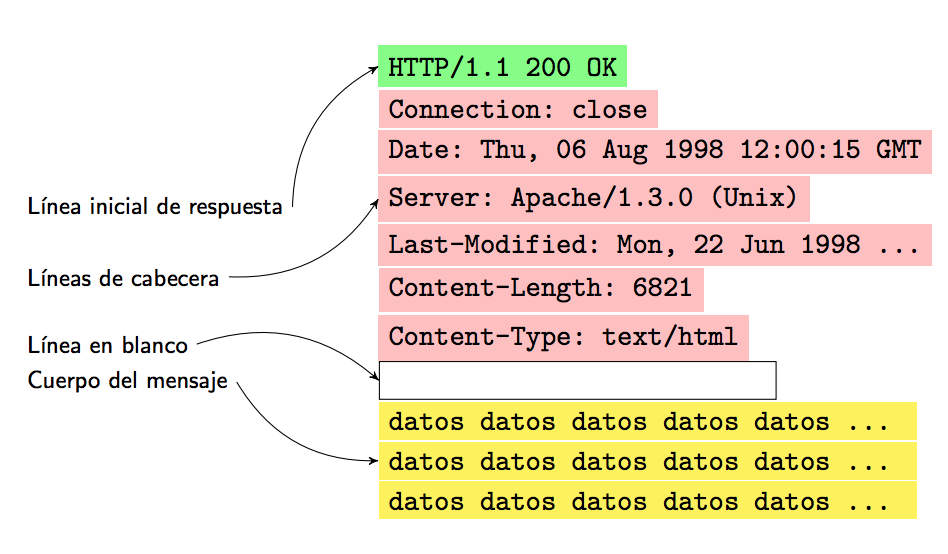
\includegraphics[width=1\columnwidth]{chapters/images/respuestahttp.png}
\caption{Ejemplo respuesta HTTP\\ Servidor a Cliente}
\end{minipage}
\end{figure}


Las dos partes que forman una aplicación web son independientes entre sí. Las tecnologías del  lado cliente (\textit{frontend}) se encargan de  interactuar con el usuario, visualizar el contenido y establecer la comunicación con el servidor. Se ejecutan en el navegador, que actúa como intérprete. Por otro lado, las tecnologías del lado servidor (\textit{backend}) se encargan de la administración del sitio web, usando bases de datos y gestores de contenidos.

Una de las principales ventajas de usar tecnologías web es que las aplicaciones creadas son multiplataforma y multidispositivo, funcionan tanto en ordenadores, móviles, tabletas, así como en distintos sistemas operativos. Otra ventaja es que no tenemos que instalar nada, sólo necesitamos el navegador y además la actualización del contenido es inmediata. El principal inconveniente es su dependencia de Internet, pero con los últimos avances tecnológicos el Wifi, la fibra óptica y el 5G han permitido que  mayoría de personas del mundo podamos acceder desde cualquier lugar y éste no sea un gran inconveniente.


\subsection{Tecnologías Web lado cliente}
Las tecnologías web del lado cliente  permiten la interacción del usuario con la página web que corre en el navegador del usuario. Para ello, se usan principalmente estas tres tecnologías \cite{tecnologiascliente}:

\begin{itemize}
  \item HTML5 \footnote{HyperText Markup Language}: es un lenguaje de marcado de los contenidos de un sitio web, se usa para asignar la función de cada elemento. Es el esqueleto de la web.
  \item JavaScript: es un lenguaje de programación interpretado que se encarga del comportamiento de una página web y de su interactividad con el usuario.
  \item CSS3\footnote{Cascading Style Sheets}: es un lenguaje de hojas de estilo creado para controlar la presentacion de la página: colores, tipo de letra, tamaños, animaciones, colocación de los elementos...
\end{itemize}

Entraremos en más detalle en estas tecnologías en el capítulo 3 donde se habla de la Infraestructura utilizada.

\newpage
\subsection{Tecnologías Web lado servidor}
Las tecnologías web del lado servidor son las que permiten gestionar y servir las páginas web y acceder a bases de datos. En este caso las tecnologías son más flexibles y vamos a nombrar tres de las más utilizadas:

\begin{itemize}
    \item Django: es un entorno para crear servidores web de alto nivel, que fomenta el desarrollo rápido con un diseño limpio y práctico en Python, destaca por su arquitectura basada en  modelo-vista-controlador y el uso de plantillas. De esta forma puedes centrarte en crear tu aplicacion web sin grandes complicaciones. Es gratis y de código abierto\cite{django}. Un ejemplo de aplicación web que utiliza Django es Instagram \cite{insta}.
    \item Node.js: es un entorno de ejecución para JavaScript orientado a eventos síncronos, construido con el motor de JavaScript V8 de Chrome. Diseñado para aplicaciones web escalables. De esta forma el cliente y el sevidor pueden crearse con el mismo lenguaje de programación\cite{node}. Netflix, Paypal o LinkedIn usan esta tecnología para sus servidores\cite{nodenetflix}. 
    
    \item PHP\footnote{Hypertext Preprocessor}: es un lenguaje de scripting de uso general popular que es especialmente adecuado para el desarrollo web\cite{php1}. Rápido, flexible y práctico, gracias a su capacidad de creación de webs dinámicas, desde blogs hasta sitios web como Facebook o Wikipedia\cite{php2}.
    
\end{itemize}

En el lado servidor se utilizan bases de datos. Una base de datos es una colección de datos estructurados. Entre ellas podemos destacar mySQL(Figura 1.11a) y MongoDB(Figura 1.11 b). 

\begin{figure}[H]
  \begin{subfigure}[b]{0.5\textwidth}
  \centering
    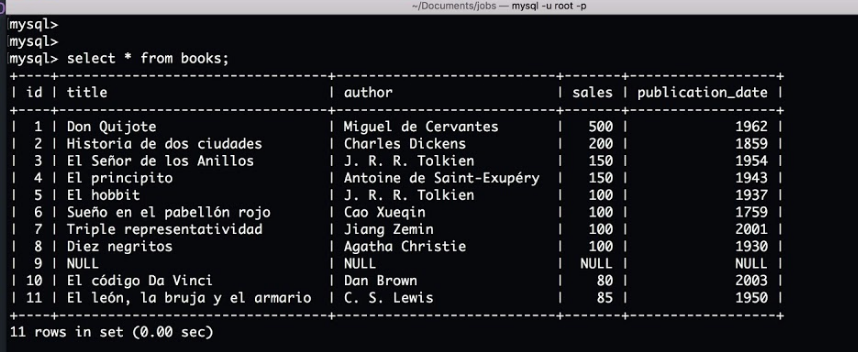
\includegraphics[width=1\textwidth, height=0.7\textwidth]{chapters/images/mysql.png}
    \caption{mySQL}
    \label{fig:f1}
  \end{subfigure}
  \hfill
  \begin{subfigure}[b]{0.5\textwidth}
  \centering
    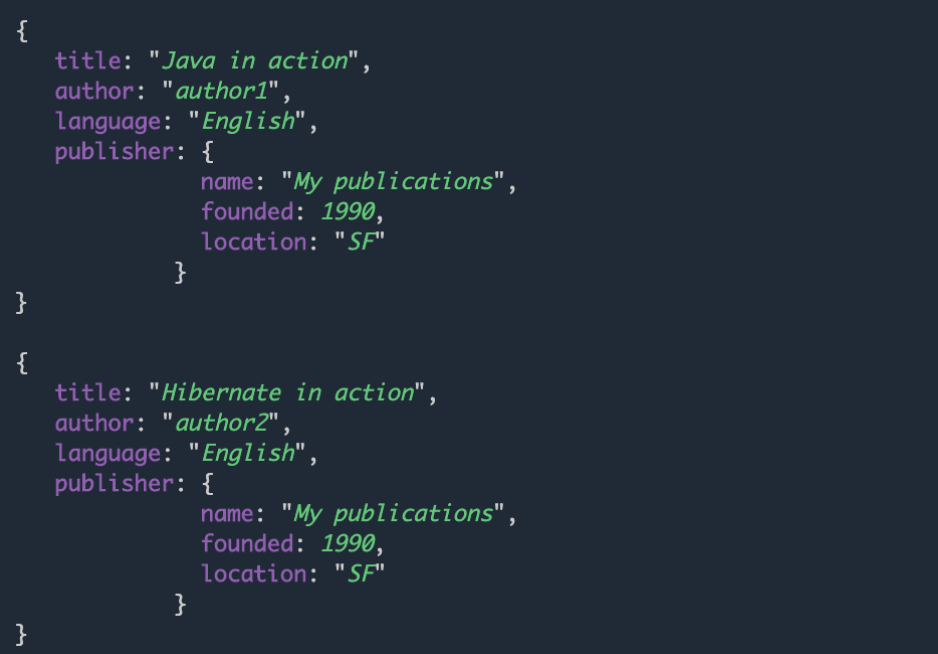
\includegraphics[width=1\textwidth, height=0.7\textwidth]{chapters/images/mongodb.png}
    \caption{MongoDB}
    \label{fig:f2}
  \end{subfigure}
  \caption{Bases de Datos}
\end{figure}



%%%%%%%%%%%%%%%%%%%%%%%%%%%%%%%%%%%%%%%%%%%%%%%%%%%%%%%%%%%%%%%%%%%%%%%%%%%%%%%%%%%%%%%%%%%%%%%%%%%%%%%%%%%%%%%%
\newpage
\section{Robótica educativa}

La Robótica educativa es un sector de aprendizaje multidisciplinar. Ayuda a desarrollar competencias y habilidades como: la innovación y espíritu emprendedor, la resolución de problemas y lógica, la toma de decisiones, conocimientos de herramientas relacionadas con las tecnologías digitales, el pensamiento crítico, creatividad, el trabajo colaborativo y cooperativo, la flexibilidad y adaptabilidad al trabajo \cite{roboticaedu}.
\\
Ante la falta de estudiantes en carreras técnicas en la actualidad, la robótica educativa puede ofrecer una gran motivación a los alumnos de las primeras etapas de educación: Primaria, ESO y Bachillerato, para fomentar la creatividad y la curiosidad al mostrar la ciencia y la tecnología de una forma diferente e incrementar sus habilidades a la vez que sus conocimientos desde los fundamentos STEM (\textit{Science, Technology, Engineering and Mathematics}).

Gracias a las tecnologías web son muchas las  aplicaciones que ofrecen cursos de robótica para todos los niveles educativos, muchos ayuntamientos están comprando cursos y materiales para facilitar a los más pequeños su introducción al mundo de la robótica a través de clases extraescolares. En secundaria se está introduciendo poco a poco en las asignaturas de tecnología el uso de lenguajes de programación, en el que destaca el lenguaje Scratch. En la Figura 1.12 podemos ver la interfaz de Scratch para programar desde el navegador.
\begin{figure}[H]
    \centering
    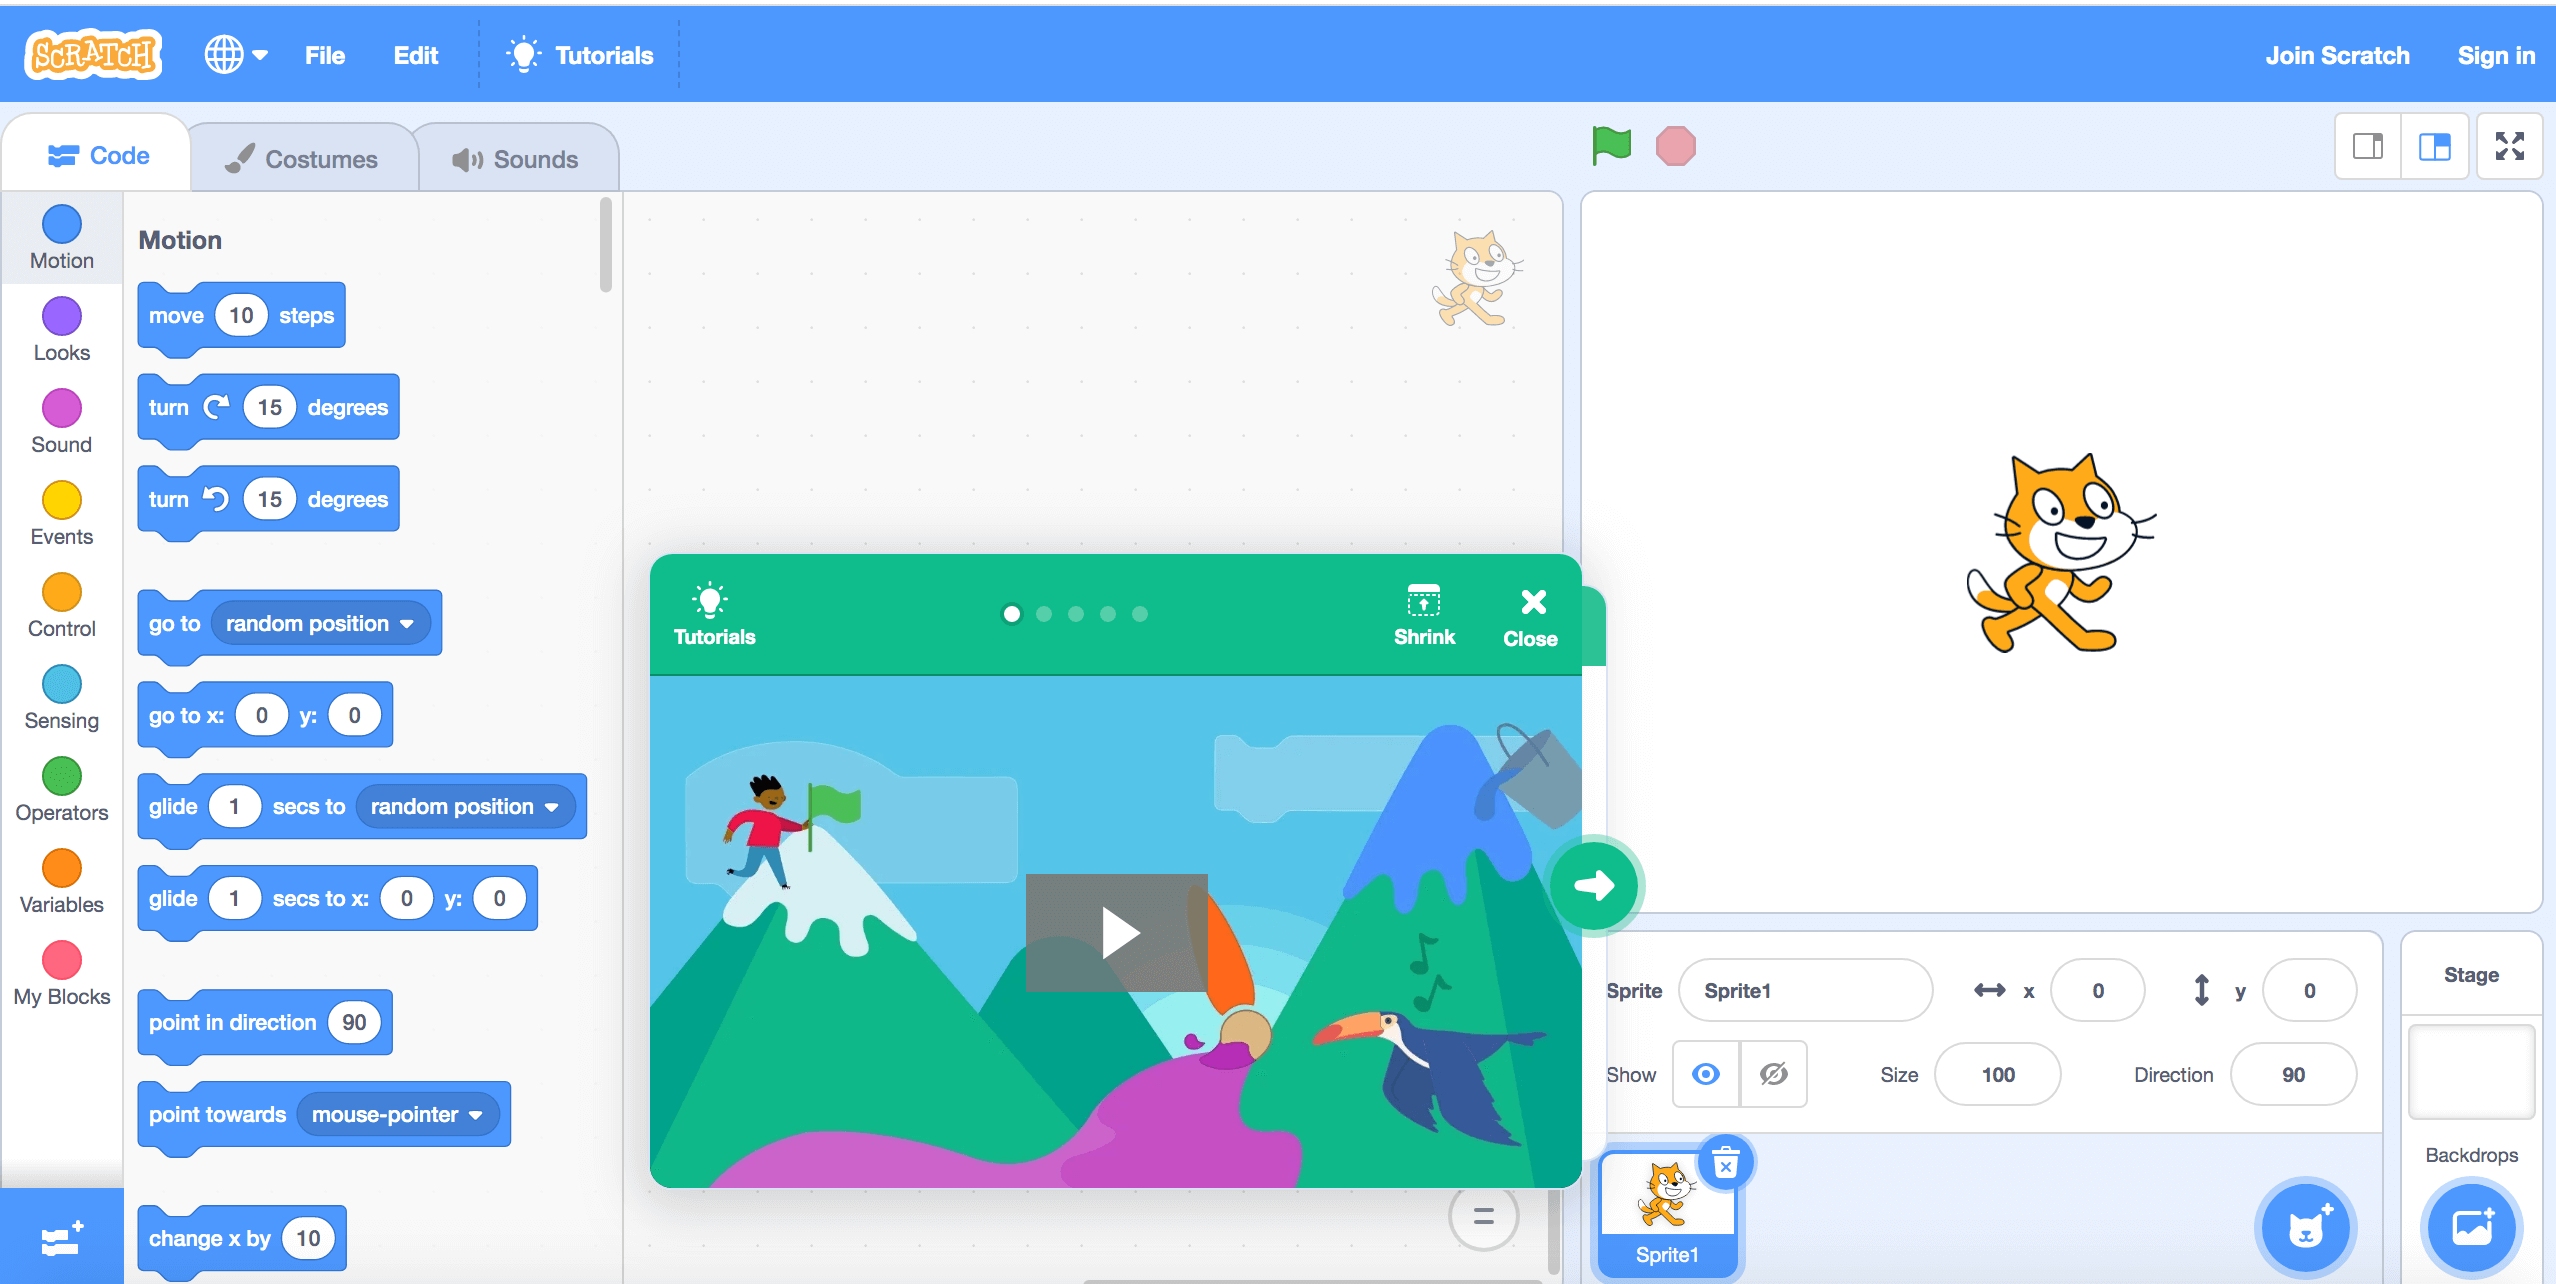
\includegraphics[width=0.8\columnwidth]{chapters/images/scratch.png}
    \caption{Scratch}
    \label{fig:my_label}
\end{figure}

Scratch es un lenguaje de programación visual basado en bloques, creado y  mantenido por Lifelong Kindergarten group en el MIT Media Lab. Scratch además es una comunidad en línea donde los niños pueden programar y compartir medios interactivos como historias, juegos y animaciones con gente de todo el mundo. Los más pequeños aprenden a pensar creativamente, trabajar en colaboración y razonar sistemáticamente\cite{scratch}. Scratch posee un lenguaje de iniciación llamado Scratch Jr pensando para niños de 5 a 7 años siendo aún más sencillo, aunque Scratch está pensado para todas las edades. Actualmente se puede utilizar desde cualquier dispositivo al ultilizar tecnologías web.

Junto con Scratch cada vez hay más plataformas y entornos STEM que se han dedicado al desarrollo de herramientas de aprendizaje enfocadas a los más pequeños. Destacan aplicaciones web como: 

\begin{itemize}
    \item  \textit{OpenRoberta \footnote{https://lab.open-roberta.org/}}: es una plataforma web creada por un instituto alemán perteneciente a la Fraunhofer Society. Tiene como objetivo simplificar conceptos de programación y facilitar a niños y profesores la codificación mediante el uso de robots como Lego Mindstorms y otros sistemas de hardware programables. \cite{openroberta}. 
    
    \begin{figure}[H]
        \centering
        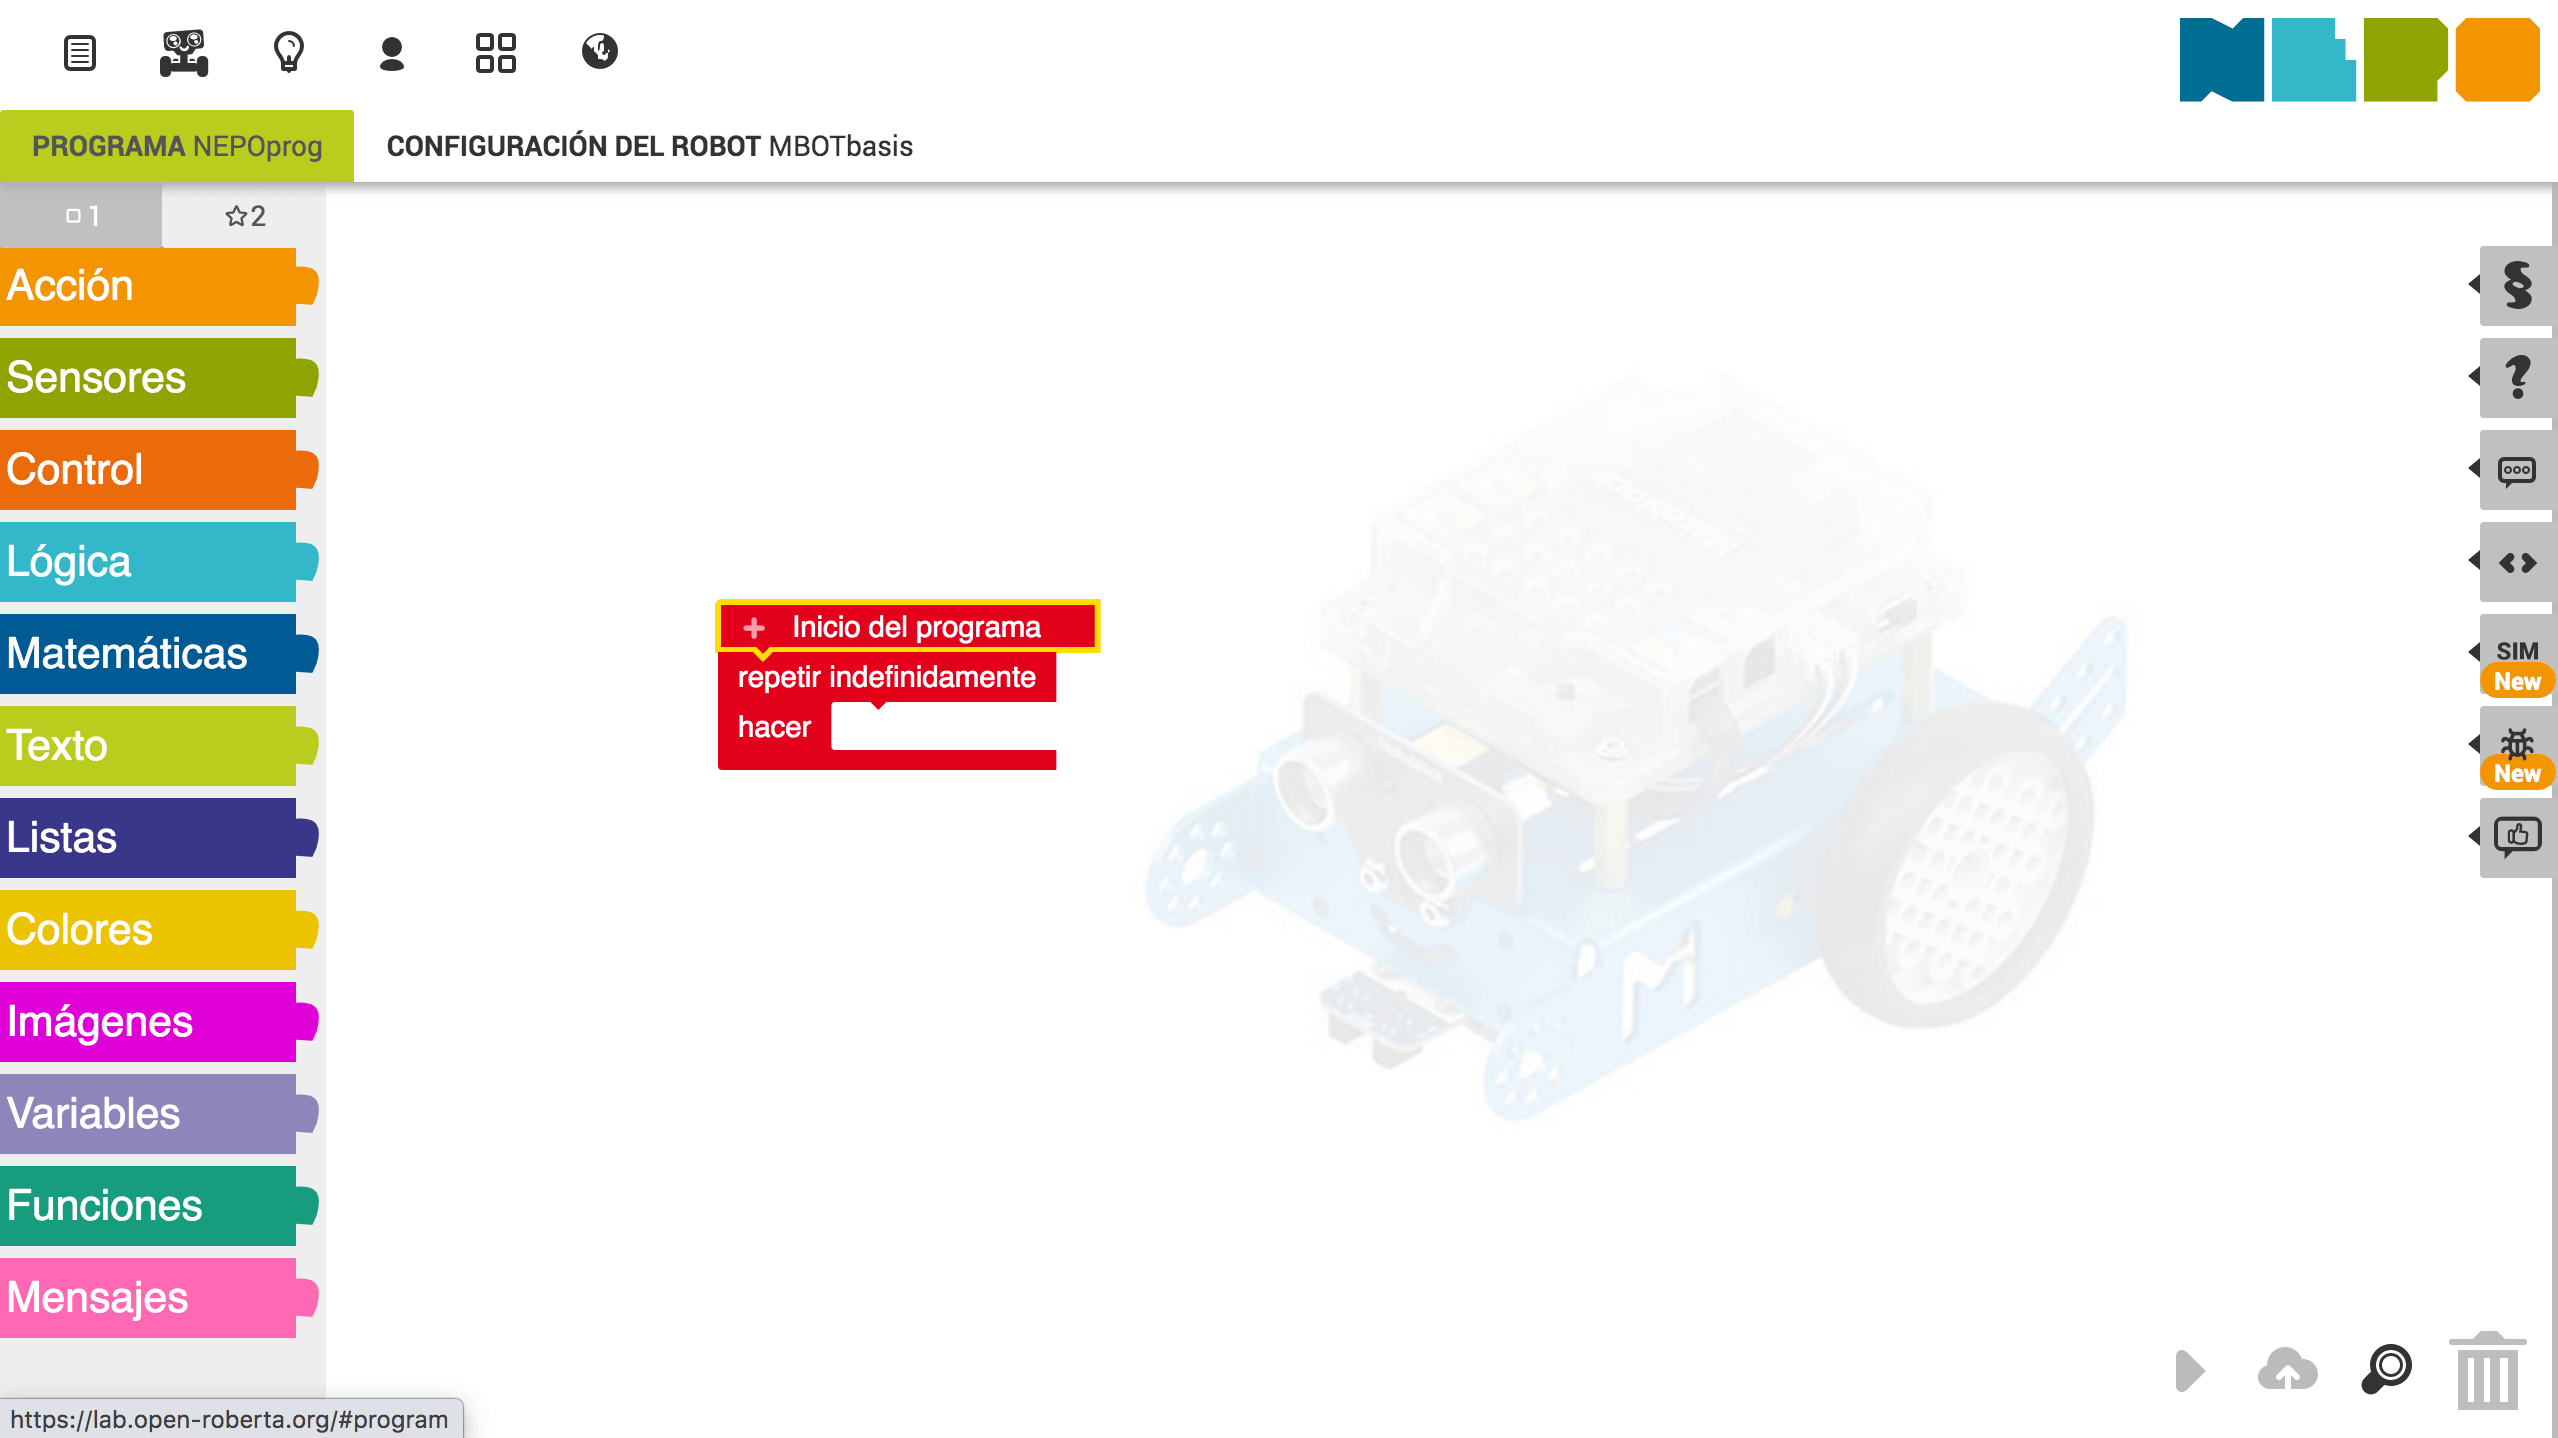
\includegraphics[width=0.7\textwidth ]{chapters/images/openrobert.png}
        \caption{Open Roberta}
        \label{fig:openroberta}
    \end{figure}
    \item \textit{LEGO Education}: la plataforma LEGO ofrece una amplia variedad de robots y \textit{packs} para uso escolar. Sus kits de robótica educativa permiten a los más pequeños construir y programar robots mediante el uso de motores, sensores, engranajes, ruedas, ejes y otros componentes técnicos, además del uso de su propio software basado en bloques. Destacan modelos como  MINDSTORMS Education EV3 y LEGO Education WeDo 2.0.\cite{ev3} \cite{legoeducation}

    \begin{figure}[H]
  \begin{subfigure}[b]{0.5\textwidth}
  \centering
    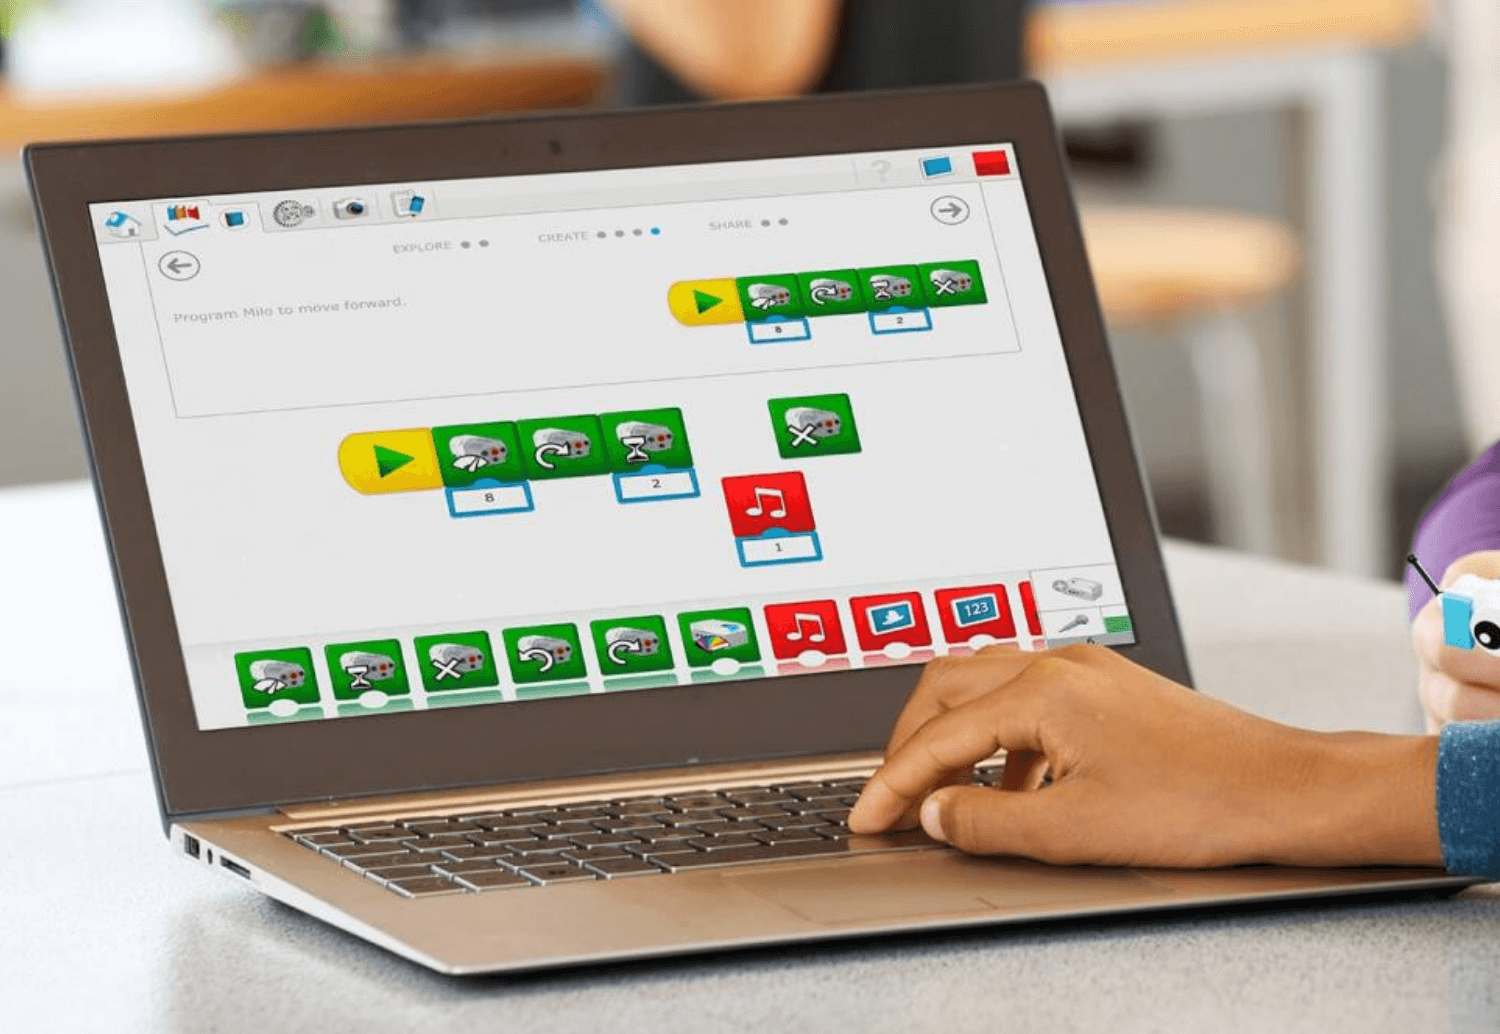
\includegraphics[width=0.9\textwidth, height=0.5\textwidth]{chapters/images/legoo.png}
    \caption{LEGO}
    \label{fig:f1}
  \end{subfigure}
  \hfill
  \begin{subfigure}[b]{0.5\textwidth}
  \centering
    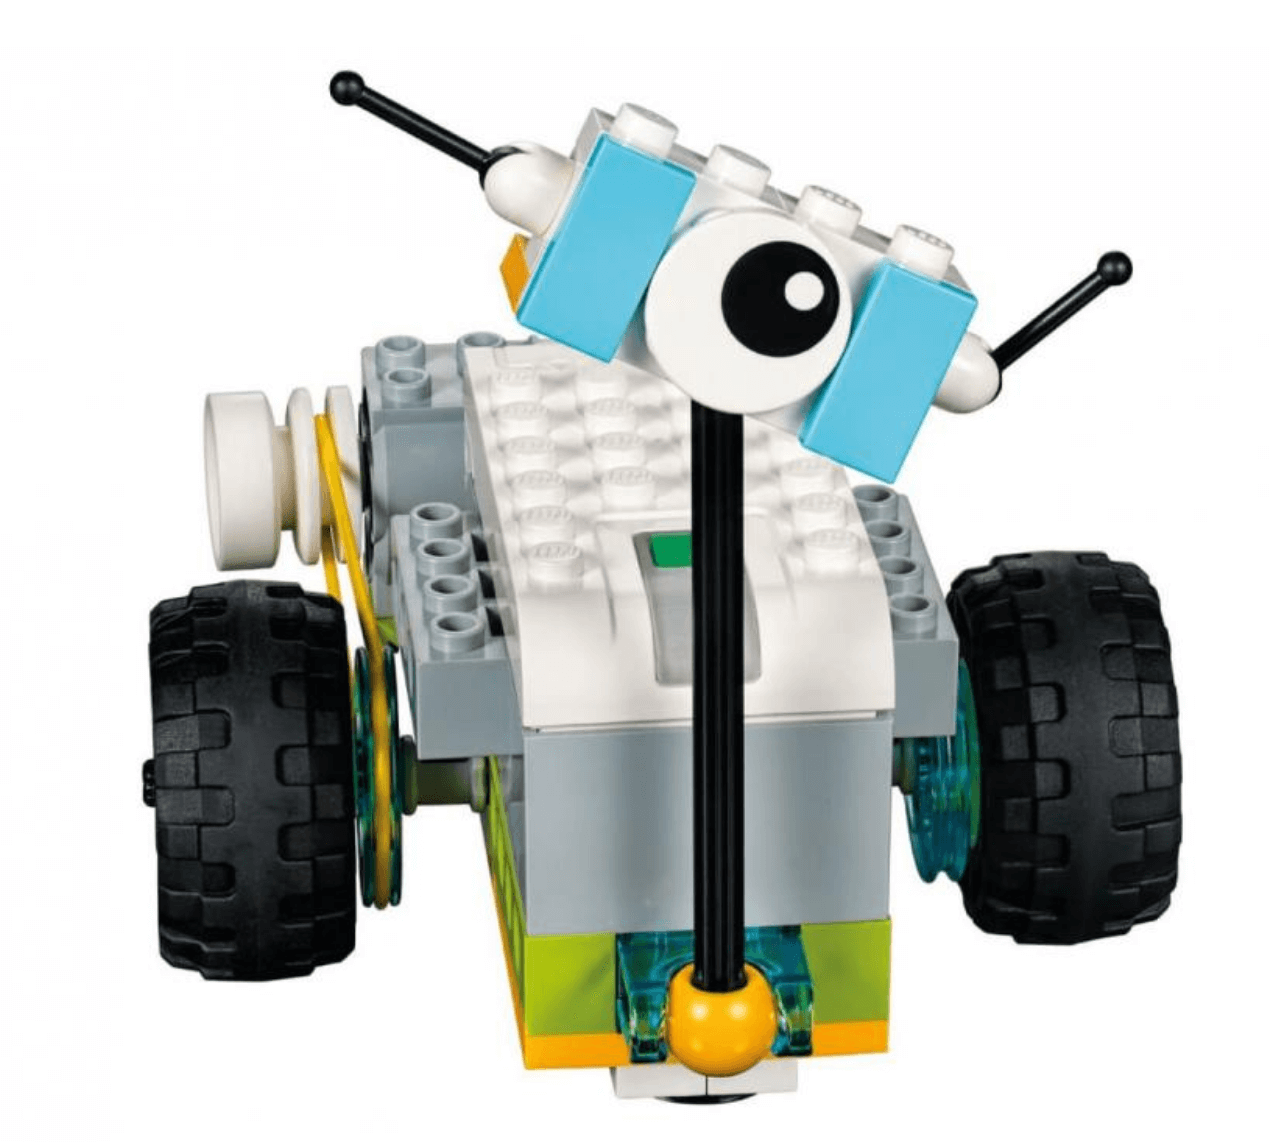
\includegraphics[width=0.9\textwidth, height=0.5\textwidth]{chapters/images/wedo.png}
    \caption{WeDo 2.0}
    \label{fig:f2}
  \end{subfigure}
  \caption{LEGO EDUCATION}
\end{figure}

    \item \textit{MBlock IDE \footnote{https://ide.mblock.cc/}}: esta aplicación web está diseñada para la educación en ciencia, tecnología, ingeniería, artes y matemáticas (STEAM). Está inspirada en Scratch 3.0, es compatible con lenguajes de programación tanto gráficos (Scratch) como textuales (Python). Se pueden diseñar historias, juegos, animaciones y programar dispositivos como robots Makeblock y microbit. \cite{mblock}
    \begin{figure}[H]
        \centering
        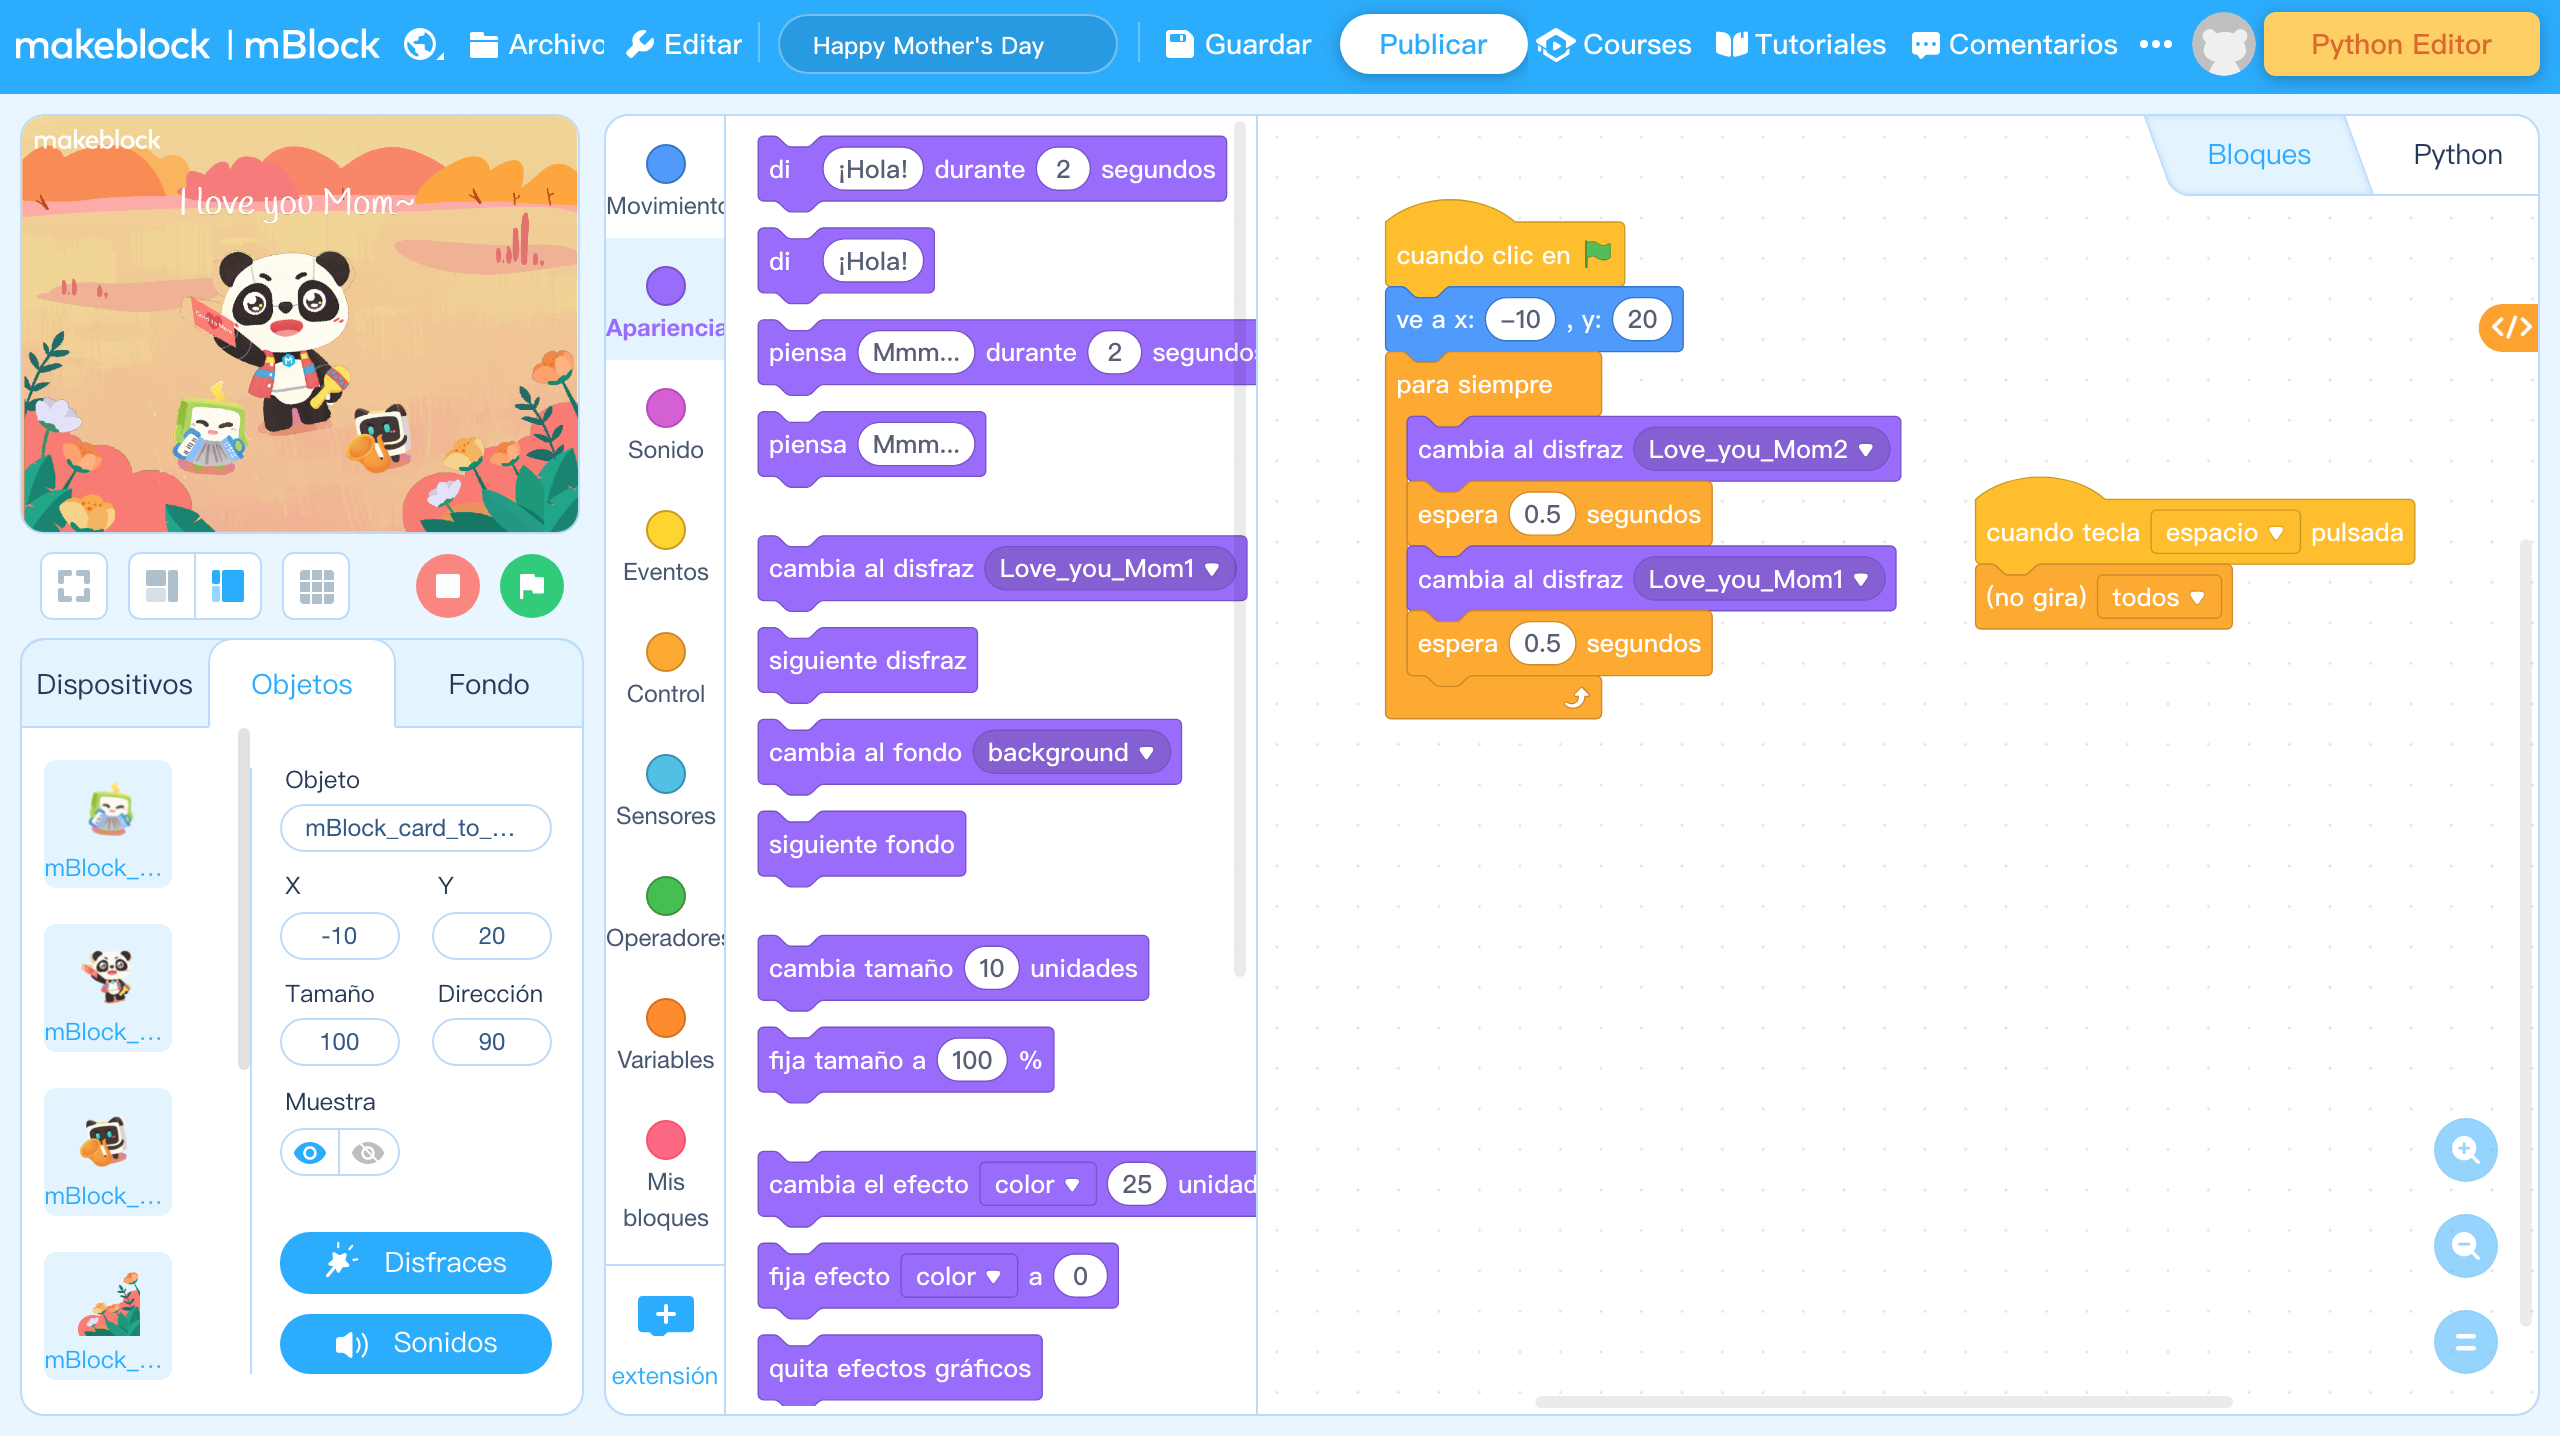
\includegraphics[width=0.7\textwidth]{chapters/images/makeblock.png}
        \caption{MBlock IDE}
        \label{fig:mblock}
    \end{figure}

    \item Vex \footnote{https://www.vexrobotics.com/}, AppInventor \footnote{https://appinventor.mit.edu/}, Arduino Web Editor\footnote{https://store.arduino.cc/digital/create}, Kodu \footnote{http://www.kodugamelab.com/} o Snap! \footnote{https://snap.berkeley.edu/} son otras plataformas web de programación en robótica educativa.
\end{itemize}


La plataforma de robótica educativa que vamos utilizar en este TFG es Kibotics. Esta plataforma, basada en tecnologías web, enseña de manera atractiva conceptos básicos de tecnología e inicia a niños y adolescentes en robótica y programación. Sigue un enfoque práctico, fomentando el pensamiento y la organización para resolver un problema, además de formar el espíritu analítico de los alumnos \cite{intro}.
\\
Actualmente ofrece cursos de robótica en Scratch y Python (Figura 1.16). En el capítulo 3 se ampliará información sobre Kibotics y veremos cómo se introduce la \textit{Gamificación} en la plataforma a lo largo de este trabajo.

\begin{figure}[H]
  \begin{subfigure}[b]{0.5\textwidth}
  \centering
    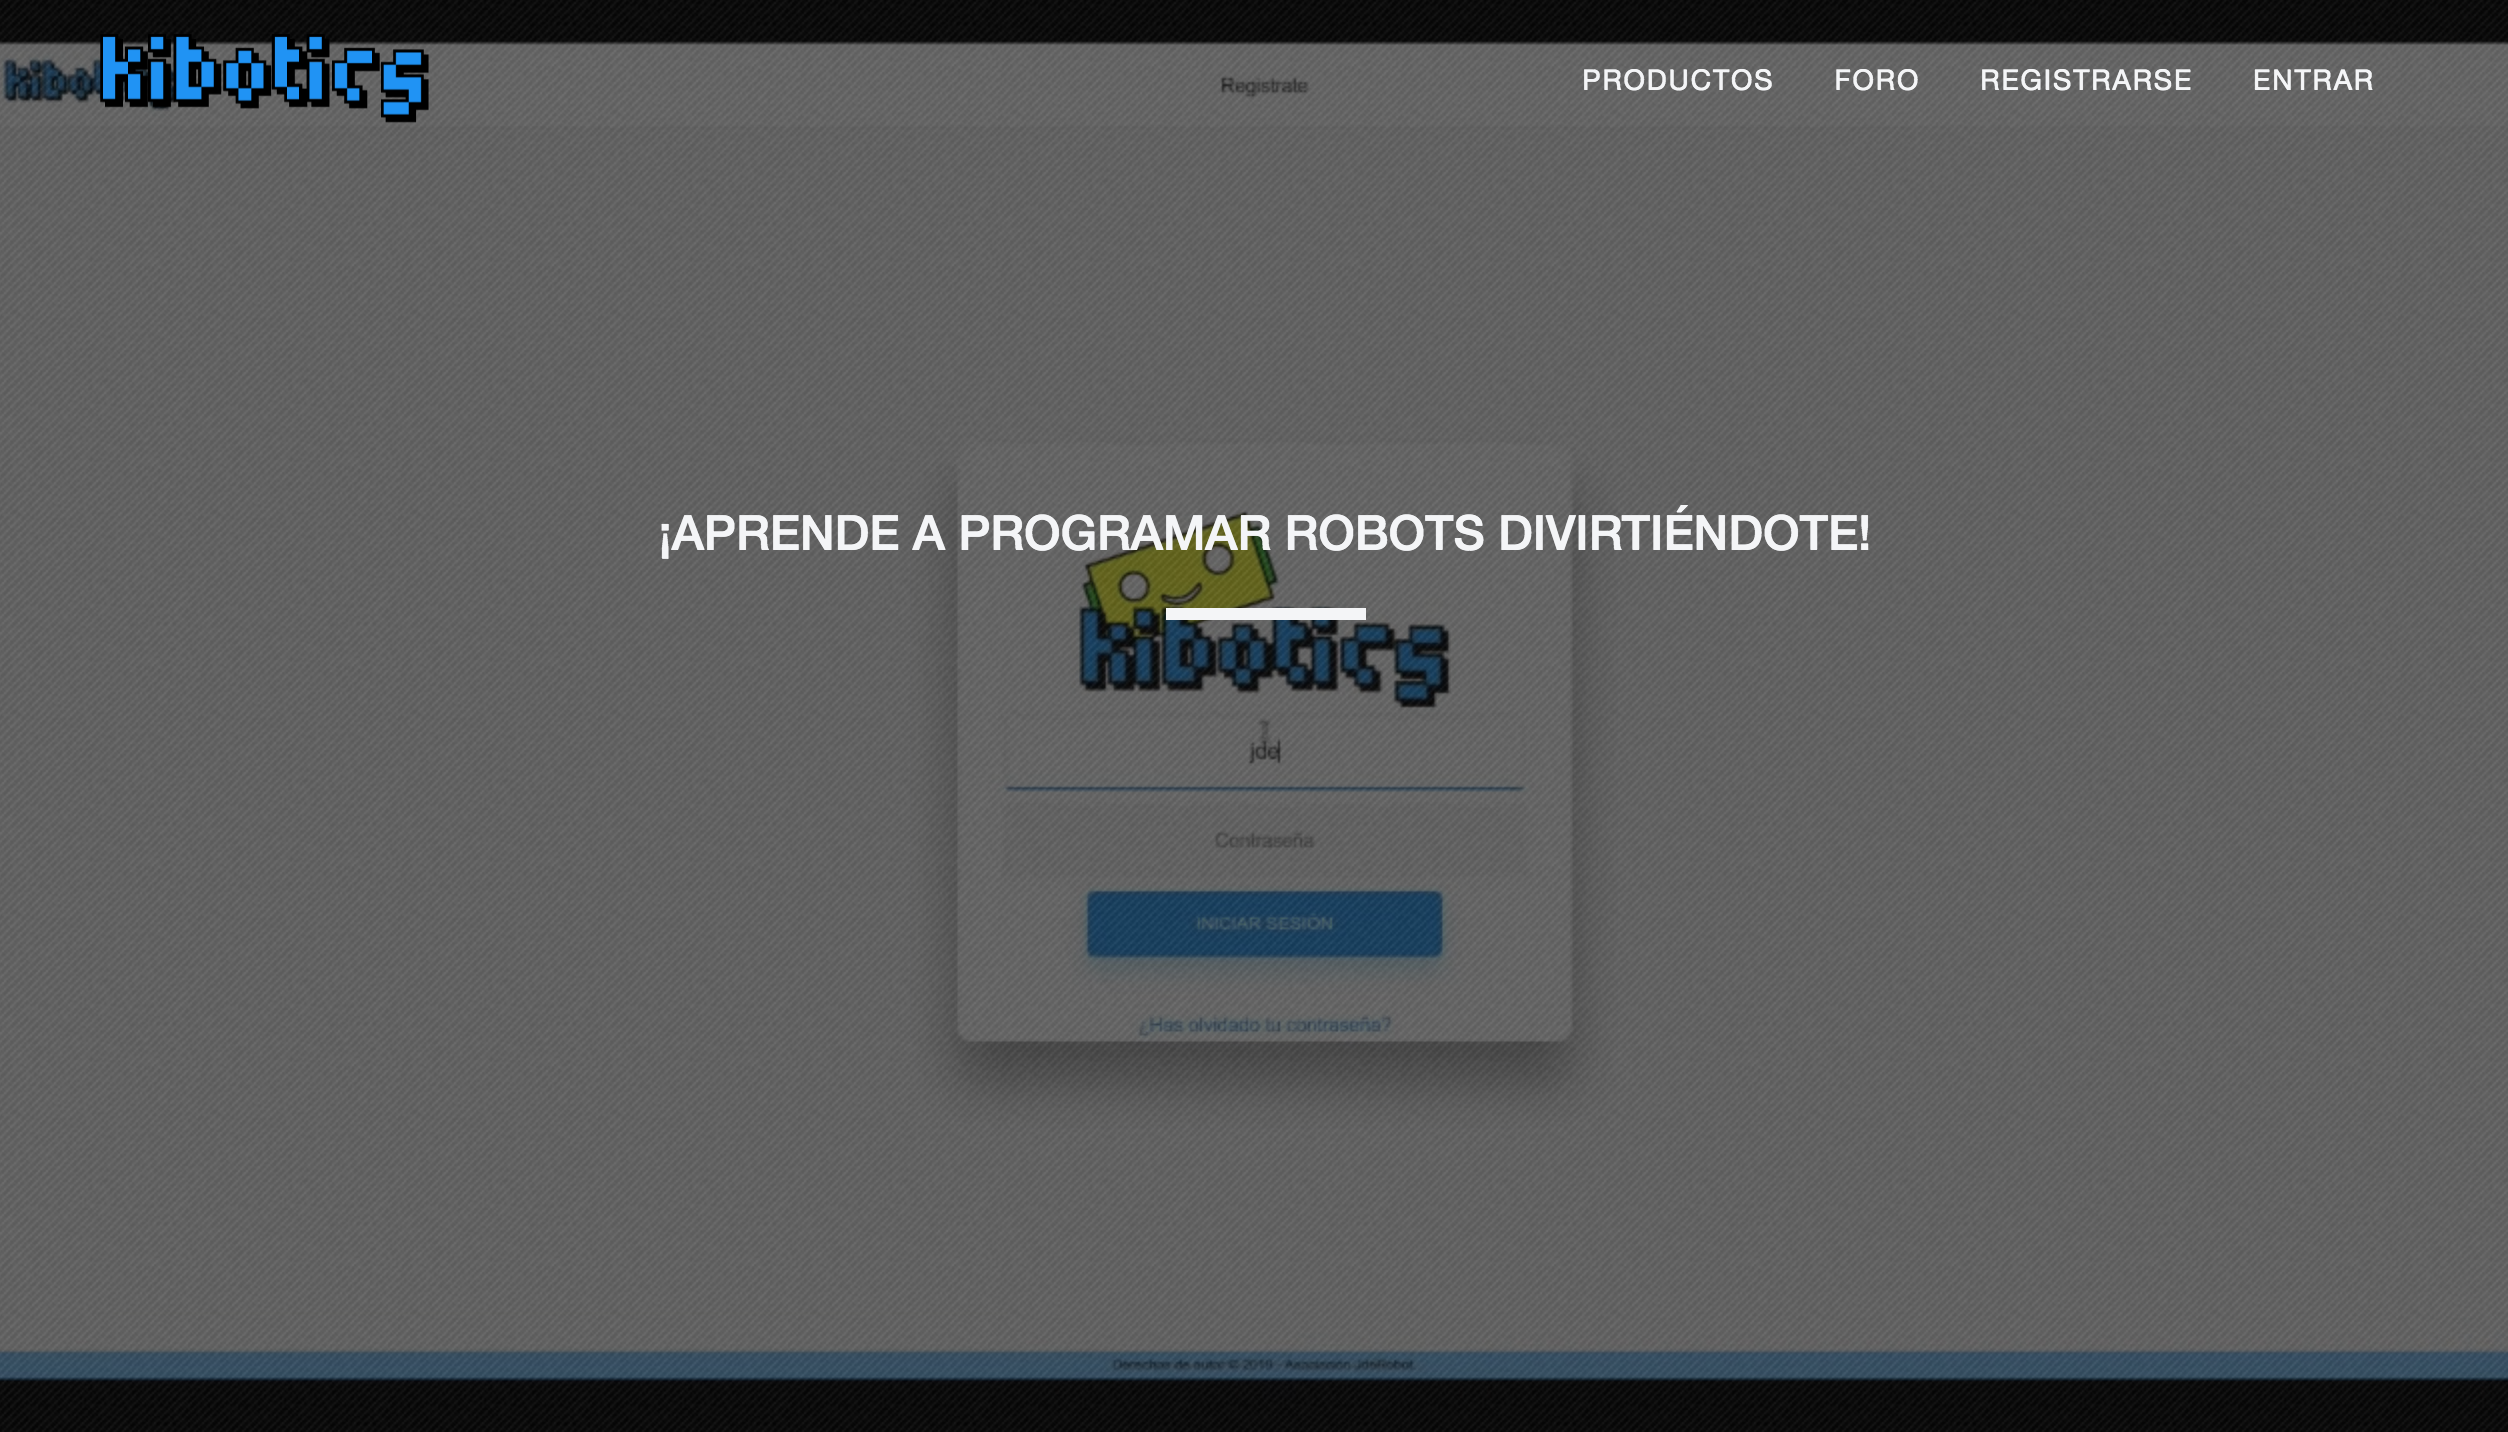
\includegraphics[width=0.9\textwidth, height=0.6\textwidth]{chapters/images/kiboticsorg.png}
    \caption{kibotics.org}
    \label{fig:f1}
  \end{subfigure}
  \hfill
  \begin{subfigure}[b]{0.5\textwidth}
  \centering
    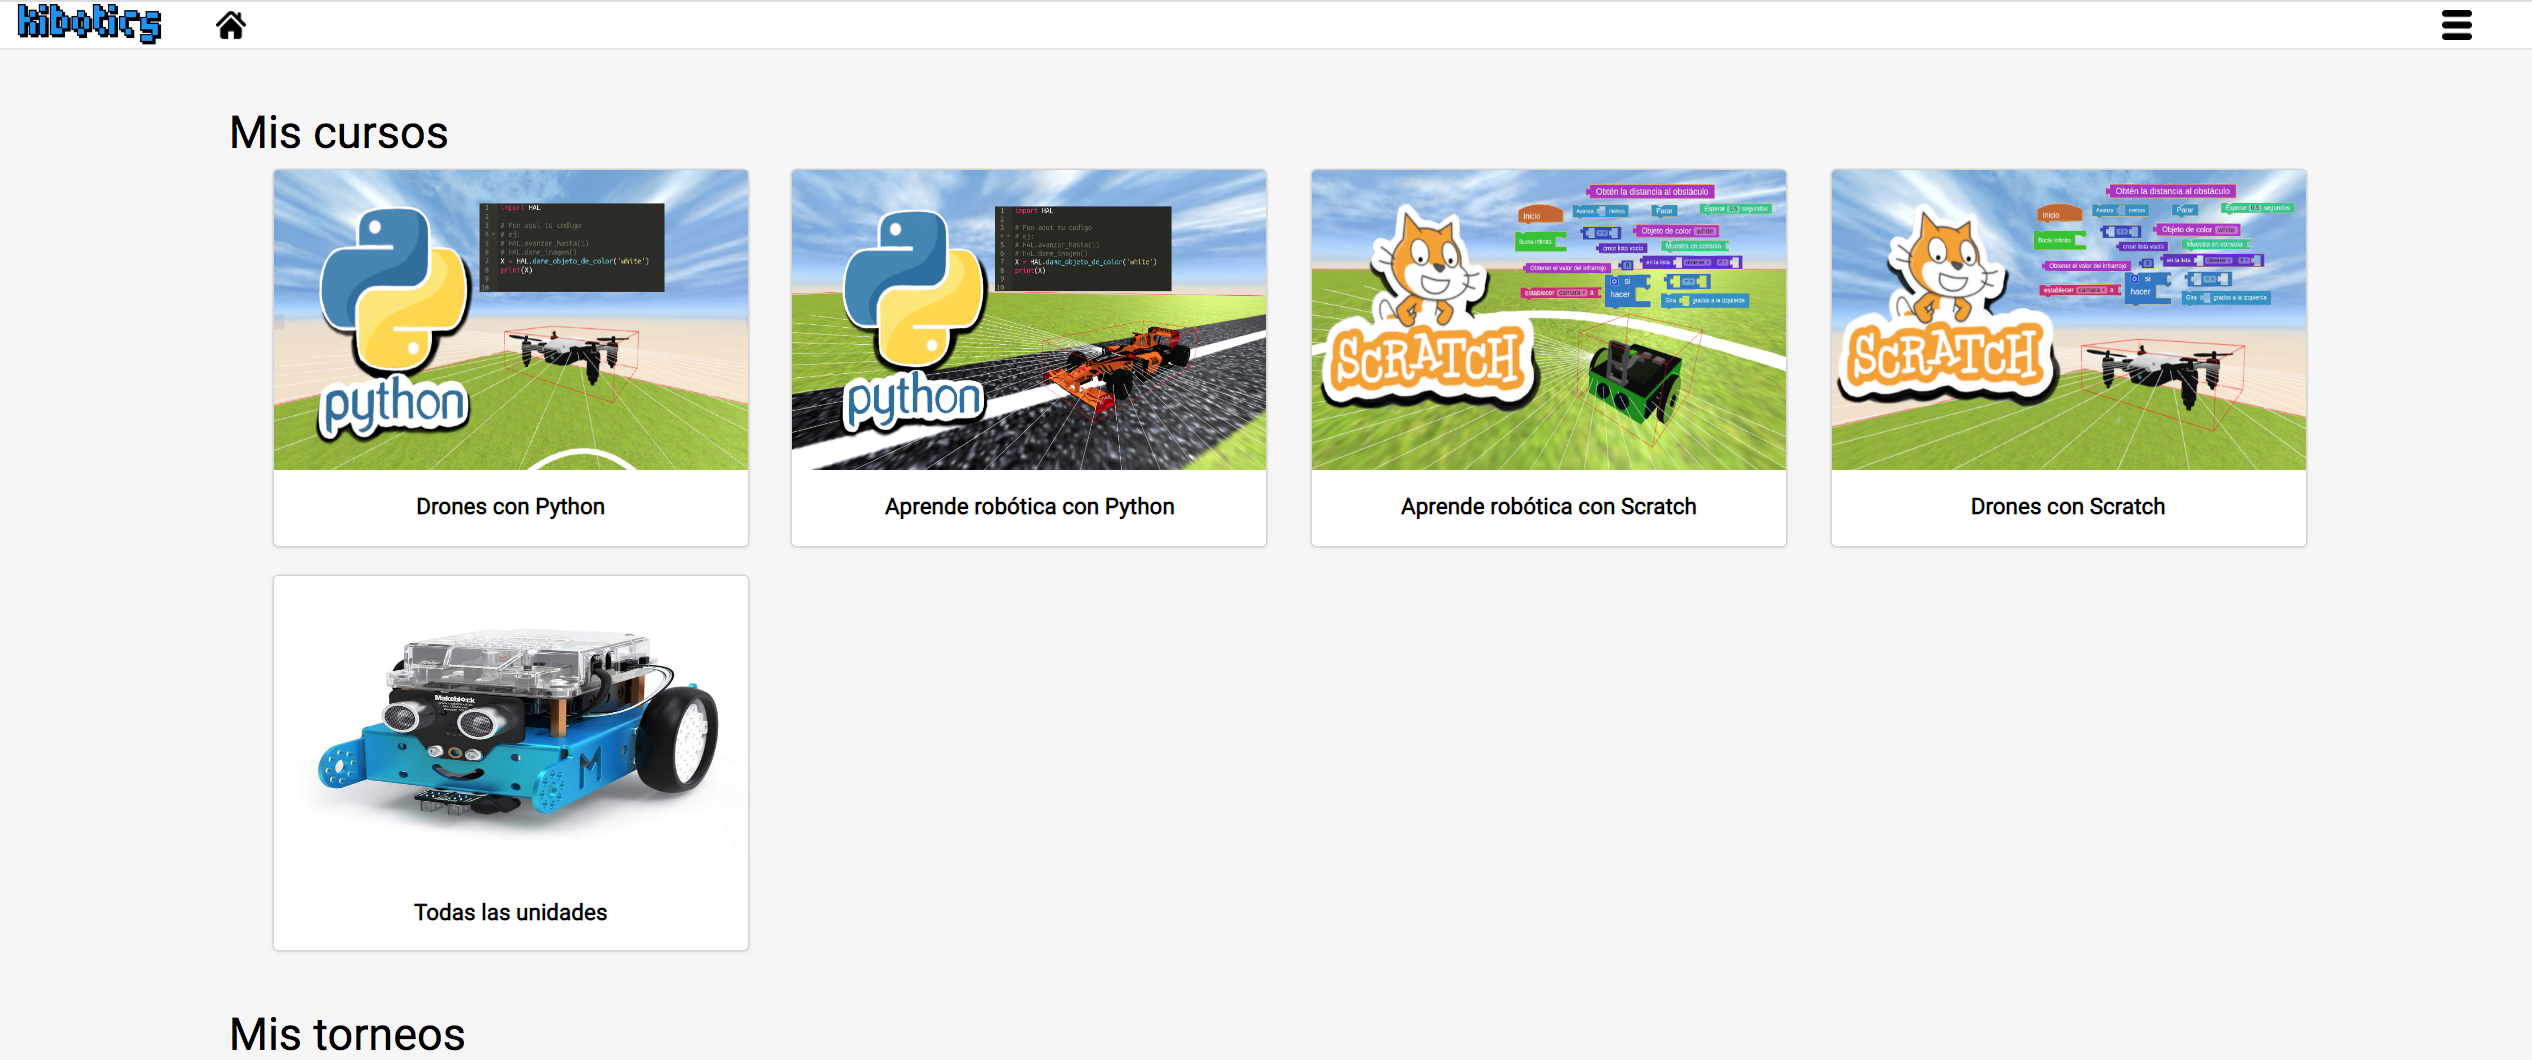
\includegraphics[width=0.9\textwidth, height=0.6\textwidth]{chapters/images/kibotics.png}
    \caption{Cursos disponibles en Kibotics.}
    \label{fig:f2}
  \end{subfigure}
  \caption{Plataforma Kibotics.}
\end{figure}
 
\subsection{Importancia de los juegos y multimedia en el aprendizaje} 
El planteamiento actual del sistema educativo tiene carencias y la innovación en la educación cobra cada vez más importancia. Es por ello que los docentes buscan actividades enfocadas en evitar la recurrente pasividad de los alumnos\cite{multimedia}.

Según concluyen el cono del aprendizaje de Edgar Dale y otros estudios, aprendemos un 10\% de lo que leemos, 20\% de lo que escuchamos, 75\% de lo que vemos y oimos y 
90\% de lo que hacemos \cite{videoeducativo}\cite{aprendizaje}. Estos porcentajes indican que, por lo tanto, la introducción del vídeo y los juegos interactivos en la clase puede producir modificaciones primordiales en el ámbito educativo.

La multimedia es un valioso recurso en la enseñanza por su naturaleza interactiva. Estos  materiales  deben ser adecuados y facilitar el aprendizaje. Para eso deben ser de fácil instalación y uso, versátiles, mostrar información de calidad e interactivos para motivar a los alumnos. Cada material se ajusta a los usuarios para que cada uno  trabaje a su ritmo \cite{importanciamultimedia}.
\\
Las nuevas tecnologías están cada vez más interiorizadas en las aulas gracias al uso de pantallas, proyectores y ordenadores. La pandemia vivida en este último año ha impulsado el uso de aplicaciones web para dar clase, como las plataformas de videoconferencia. Muchos profesores han optado por estas potentes plataformas, otros han grabado y compartido sus propios vídeos, donde los estudiantes pueden pararlos y verlos las veces necesarias para interiorizar mejor los conocimientos.
\\
En los últimos años se están incorporando juegos en las aulas como la apliación Kahoot! \cite{kahoot} en la que hacen juegos de encuestas, además se ha fomentado aprendizaje a través de vídeos y diapositivas más animadas, foros, así como el uso de plataformas educativas e interactivas como Moodle.
\\

 El término \textit{``Gamificación''} o ludificación se emplea para referirse al aprendizaje a través de juegos en el entorno educativo y profesional. Los juegos se utilizan para fomentar el aprendizaje de programación, mejorando los conocimientos y habilidades de los alumnos de una forma más dinámica y divertida. La Gamificación facilita la interiorización de los conocimientos, generando una respuesta positiva al usuario por cumplir con un objetivo.
 \\
 Enseñar a los más jóvenes cómo funcionan las últimas tecnologías y que además les parezca entretenido e interesante es lo que nos ha motivado a realizar este trabajo.
 
 
\subsection{Campeonatos de robótica educativa existentes}

El aprendizaje de la robótica educativa ha ido más allá. Actualmente existen competiciones a nivel nacional e internacional que utilizan juegos y ejercicios competitivos \cite{competiciones}. Estas son algunas de ellas:
\begin{itemize}
    \item RoboCup Junior \footnote{https://junior.robocup.org/}: es una iniciativa educativa orientada a proyectos que patrocina eventos robóticos locales, regionales e internacionales para jóvenes estudiantes. Destaca la Liga de Rescate, Liga de Futbol (Figura 1.17(b)) y Liga ONSTAGE \cite{robocup}.
 
    \item Eurobot Junior\footnote{http://www.eurobot.es/}: es una competición europea de robots para estudiantes de primaria, secundaria o clubs de robótica. El grupo de jóvenes debe diseñar, construir y programar un robot telecontrolado por cable. Además pueden tener un robot secundario autónomo\cite{eurobot}.
    
    \item First Lego league \footnote{https://www.firstlegoleague.es/}: es un programa internacional  para jóvenes de 4 a 16 años a través de la resolución de problemas reales. Se adapta a cada edad con sus cursos Discover, Explore y Challenge\cite{firstlego}.
    
    \item Torneo Nacional VEX Robotics IQ\footnote{https://vexspain.com/}: destinado a equipos de 4 a 8 miembros de secundaria junto un adulto. Ofrecen distintos retos y torneos con premios\cite{vex}.
    
    \item RoboCampeones \footnote{http://robocampeones.org/}: Creado en el RoboticsLabURJC de la Universidad Rey Juan Carlos. Los alumnos de instituto compiten en pruebas como sumo con robots LEGO y Arduino. Se celebra en Fuenlabrada y en los últimos años contó con más de 2000 participantes (Figura 1.17(a)) \cite{robocampeones}.
    \\
    \\
    
    \begin{figure}[H]
  \begin{subfigure}[b]{0.5\textwidth}
  \centering
    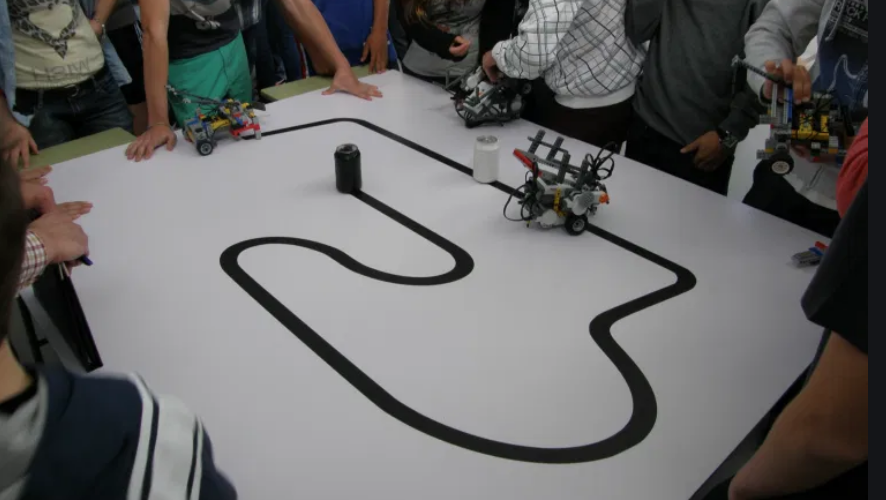
\includegraphics[width=0.95\textwidth, height=0.7\textwidth]{chapters/images/robocam.png}
    \caption{Juego Pañuelo Robocampeones}
    \label{fig:f1}
  \end{subfigure}
  \hfill
  \begin{subfigure}[b]{0.5\textwidth}
  \centering
    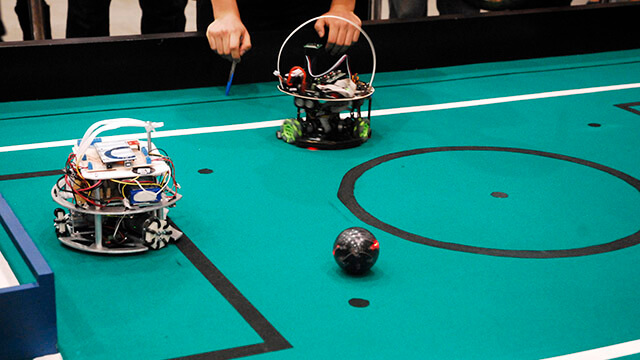
\includegraphics[width=0.95\textwidth, height=0.7\textwidth]{chapters/images/robocup.jpeg}
    \caption{Fútbol en RoboCup Junior.}
    \label{fig:f2}
  \end{subfigure}
  \caption{Campeonatos de robótica.}
\end{figure}
\end{itemize}

\newpage
\section{Estructura del documento}

La estructura de este trabajo fin de grado está compuesta por los siguientes capítulos:

\begin{itemize}
    \item \textit{Capítulo 1 Introducción}: una breve introducción a la robótica y tecnologías web para ponernos en contexto y presentar el tema principal del trabajo.
    \item \textit{Capítulo 2 Objetivos y Metodología}: Se fijan los objetivos concretos y se explica la metodología y plan de trabajo seguidos a lo largo de este proyecto.
    \item \textit{Capítulo 3 Infraestuctura utilizada}: se describen lenguajes, tecnologías y herramientas empleadas en este trabajo.
\end{itemize}

Para una mejor exposición del trabajo que se ha realizado, el desarrollo se ha dividido en 3 Capítulos. De esta forma nos centraremos en el enunciado, la infraestructura y solución de referencia de cada ejercicio:
    
\begin{itemize}
   \item \textit{Capítulo 4 Ejercicio Teleoperador Acústico y Banda Sonora}
    \item \textit{Capítulo 5 Ejercicio Aspiradora robótica atrapa confeti}
    
    \item \textit{Capítulo 6 Ejercicio Juego del pañuelo}

    
    \item \textit{Capítulo 7 Conclusiones y trabajos futuros}: Conclusiones del trabajo y futuros proyectos posibles a partir de éste.
  \end{itemize}


% OBJETIVOS %
%%%%%%%%%%%%%%%%%%%%%%%%%%%%%%%%%%%%%%%%%%%%%%%%%%%%%%%%%%%%%%%%%%%%%%%%%%%%%%%%
\chapter{Objetivos y Metodología del Trabajo}\label{objetivos}

En este capítulo se plantean los objetivos a cumplir con este proyecto, así como los requisitos, metodología y el plan de trabajo que se ha seguido para alcanzarlos.

\section{Objetivos}

El objetivo principal de este trabajo es introducir la gamificación en la plataforma Kibotics, para ello, vamos a centrarnos en los siguientes subobjetivos u objetivos específicos a cumplir:

\begin{itemize}
    \item Diseñar y desarrollar un nuevo juego que analice el audio en tiempo real y explorar la posibilidad de añadir bandas sonoras a los ejercicios actuales. 

    \item Diseñar y desarrollar un nuevo ejercicio sobre una aspiradora robótica que tiene que limpiar una habitación.

    \item Diseñar y desarrollar un nuevo ejercicio sobre un robot que juega al pañuelo, recorriendo una línea, una lata que ejerce de pañuelo y regresando con ella al lugar de partida.

    Para los tres ejercicios se desarrollará la infraestructura necesaria, modelos nuevos de robot, escenarios en el simulador, evaluadores automáticos, soluciones de referencia y se integrarán en la plataforma web de robótica eduactiva Kibotics.
    
\end{itemize}


\newpage

\section{Requisitos}
Para cumplir con los objetivos citados anteriormente debemos tener en cuenta además los siguientes  requisitos: 
\begin{itemize}
    \item Los robots y juegos desarrollados deben ser compatibles con la versión actual v.2.8 o superior de Kibotics.
    \item No se debe requerir de instalaciones adicionales. Todo debe correr en el navegador web del cliente. 
    \item Uso de software de simulación Websim y A-Frame.
\end{itemize}

 
\section{Metodología}

La metodología que se ha seguido para la realización de este trabajo es la basada en el modelo de desarrollo software iterativo y creciente (Figura 2.1) \cite{modeloiter}.
Este modelo consiste en entregar a los usuarios y al equipo de desarrolladores de Kibotics, una versión usable lo antes posible y en continua actualización. En cada iteración se van solventando pequeños errores y mejoras que convergen en la versión final del proyecto.

\begin{figure}[H]
    \centering
    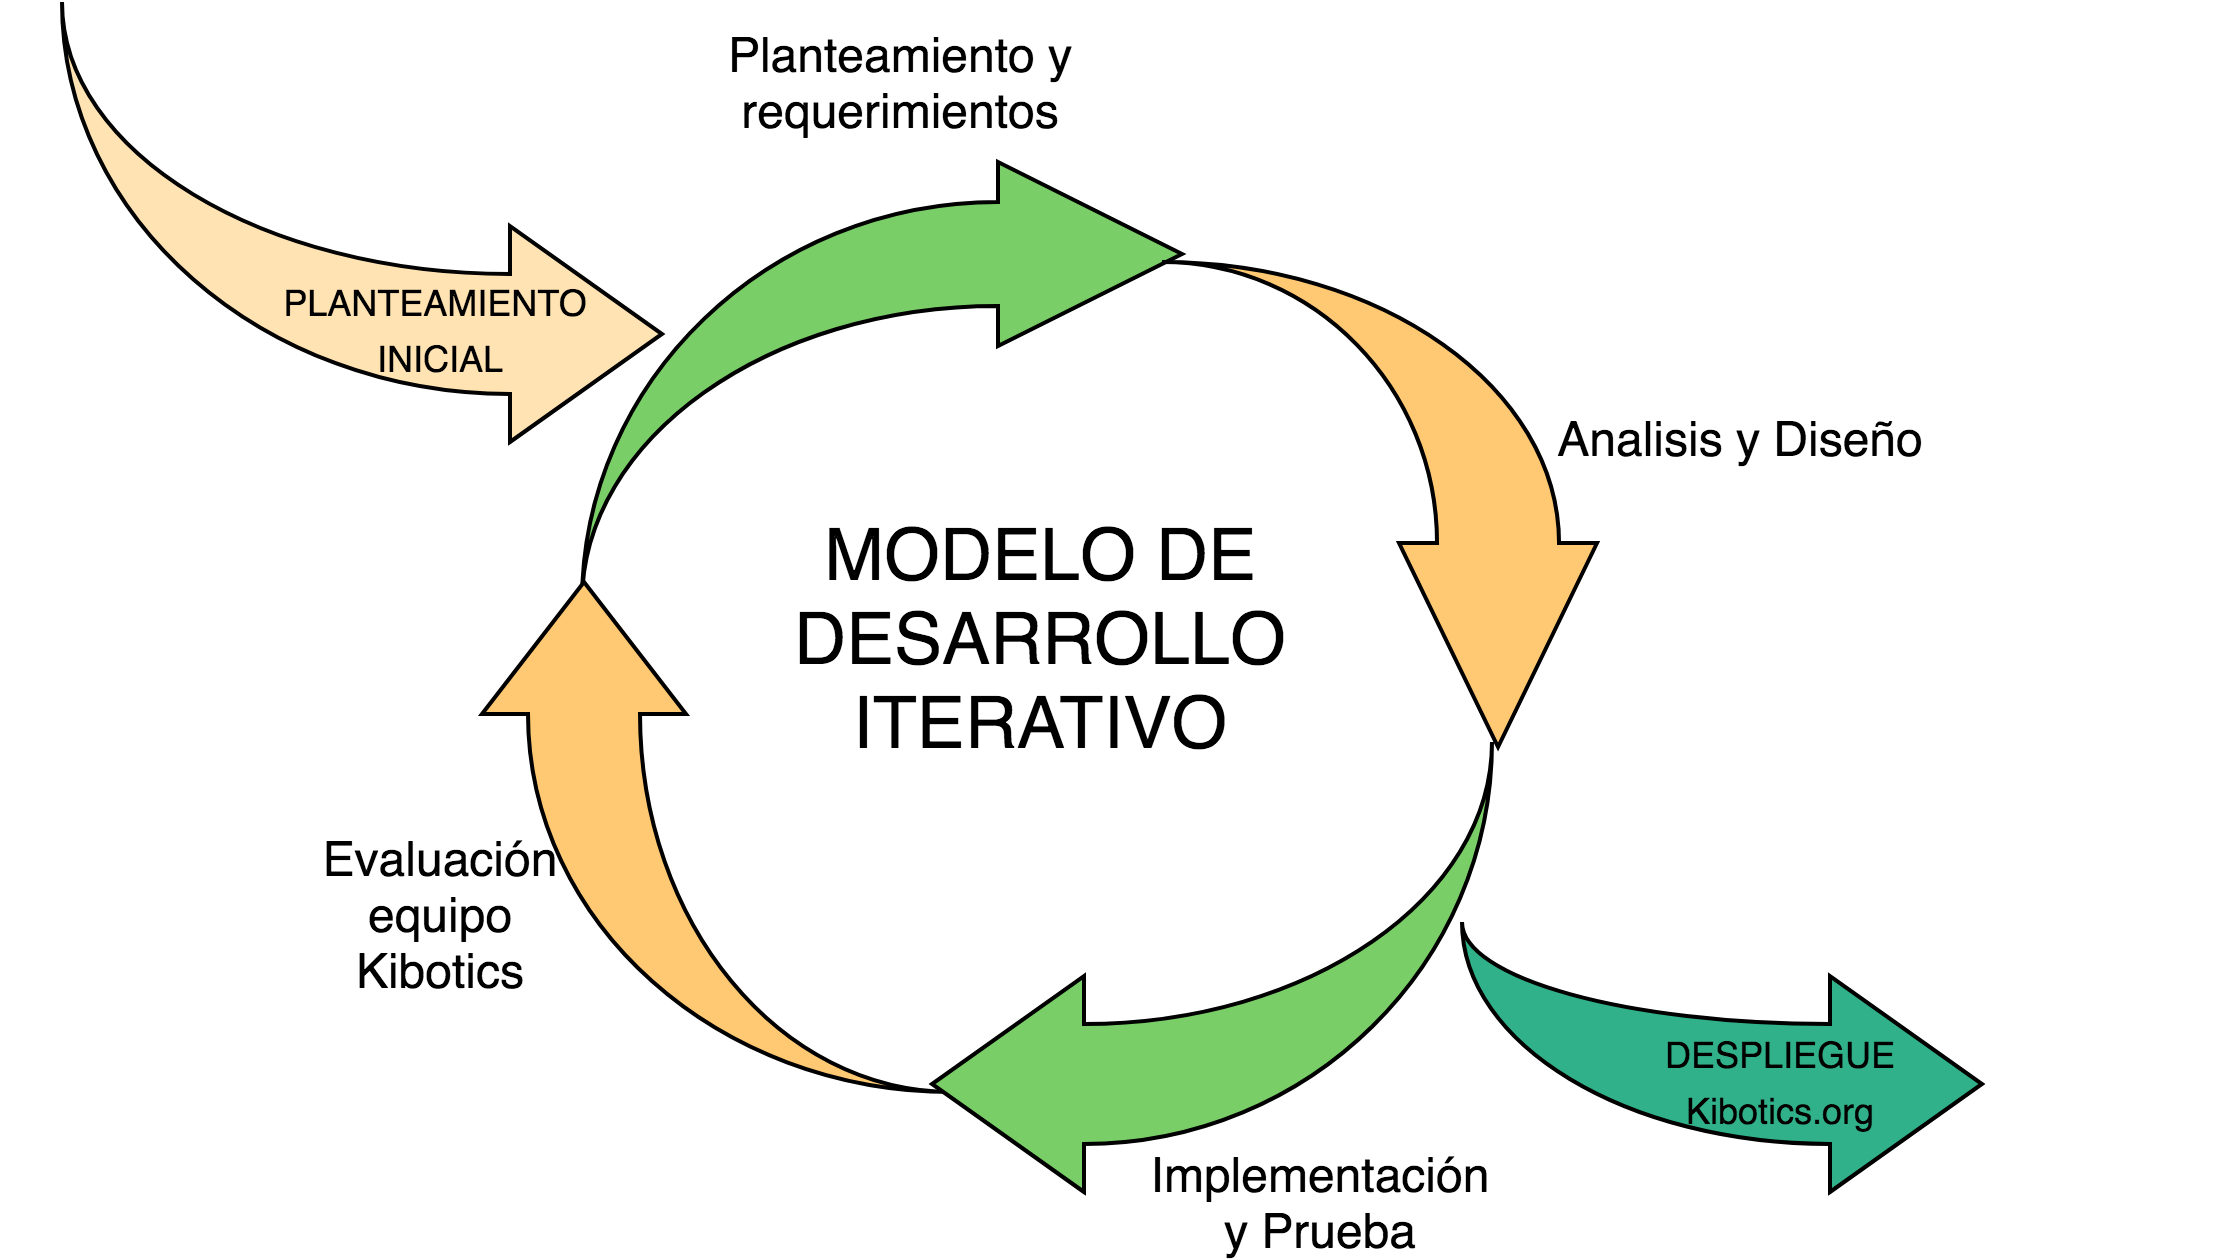
\includegraphics[width=0.6\columnwidth]{chapters/images/metodologiaiterativa.png}
    \caption{Modelo iterativo}
    \label{fig:my_label}
\end{figure}


El código desarrollado y las mejoras se han integrado progresivamente en el código fuente oficial de Kibotics en GitHub \footnote{https://github.com/} mediante su flujo de trabajo  incidencia (\textit{issue}), rama (\textit{branch}) y parche (\textit{pullresquest}). De esta forma la plataforma oficial está siempre actualizada con los últimos cambios añadidos y verificados por el equipo de desarrolladores.

Para llevar acabo esta metodología se establecieron reuniones semanales con el tutor para la orientación de este trabajo fin de grado. A lo largo del proyecto se ha mantenido la comunicación con el tutor y el equipo de Kibotics a través de la plataforma Slack \footnote{https://slack.com/}. 



Además se ha creado una página web tipo blog para llevar un seguimiento de las tareas realizadas y los objetivos semanales. \footnote{https://roboticslaburjc.github.io/2020-tfg-marta-quintana/}

\begin{figure}[H]
    \centering
    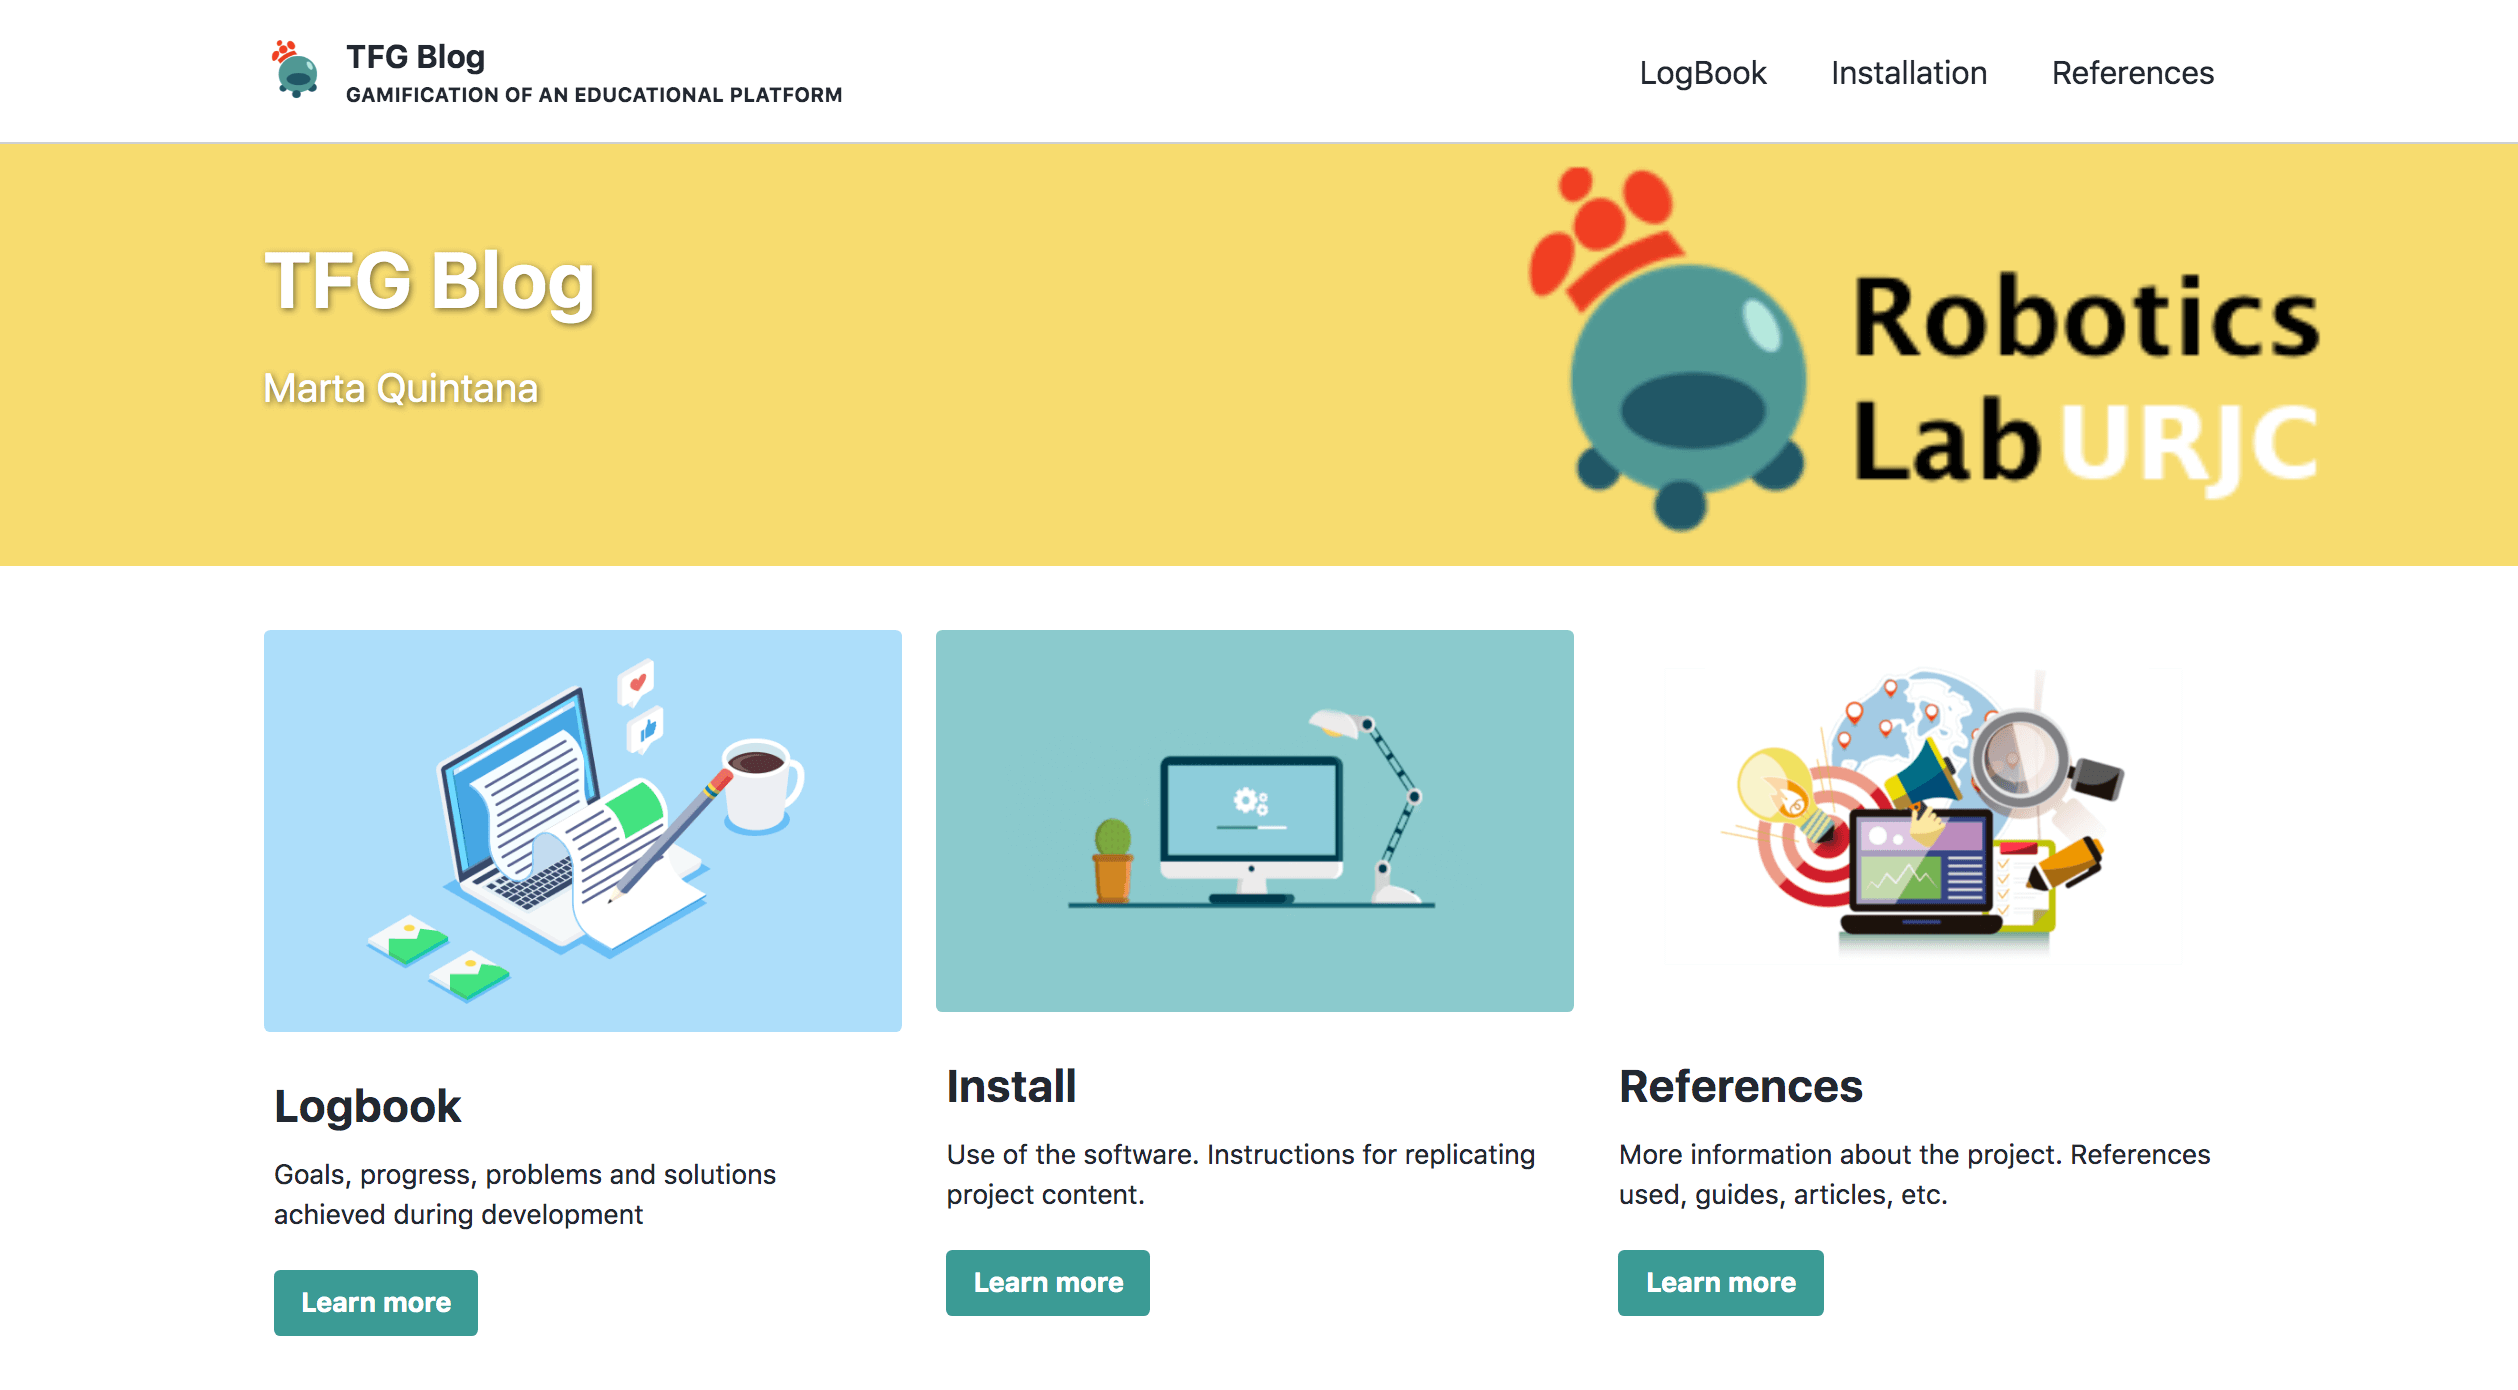
\includegraphics[width=0.6\linewidth]{chapters/images/webtfg.png}
    \caption{Página web de este TFG}
    \label{fig:my_label}
\end{figure}

\section{Plan de Trabajo}
El plan de trabajo seguido durante este proyecto se puede dividir en las siguientes etapas:


\begin{itemize}
    \item \textbf{Aterrizaje en Kibotics y repaso de tecnologías web}: Toma de contacto con Kibotics y repaso de HTML5, JavaScript, Django y otras tecnologías que se utilizan en la plataforma.
    
    \item \textbf{Estudio Web Audio API y Tensor FlowJS}: Realización de ejercicios y tutoriales de distintas herramientas para introducir sonido y reconocimiento de audio en Kibotics.
   
    \item \textbf{Diseño Teleoperador Acústico con Teachable Machine}: Creación de un teleoperador acústico con reconocimiento de audio. 

    \item \textbf{Prototipo de aspiradora robótica}: Diseño y creación de modelos del nuevo ejercicio.
    \item \textbf{Diseño ejercicio aspiradora robótica confeti}: Desarrollo de una aspiradora robótica simulada, un nuevo actuador de absorción y piezas de confeti que puedan ser absorbidas por la aspiradora.
    
    \item \textbf{Prototipo ejercicio Mbot con Pinza basado en A-Frame}: Creación de un prototipo en A-Frame nativo para el estudio de las físicas y mallas de colisión. 
    \item \textbf{Preparación del ejercicio del pañuelo}: Creación e implementación del ejercicio, desarrollo del circuito, una lata y un Mbot con Pinza realizados con Blender y JavaScript, para ofrecernos físicas más realistas.

\end{itemize}



% HERRAMIENTAS %
%%%%%%%%%%%%%%%%%%%%%%%%%%%%%%%%%%%%%%%%%%%%%%%%%%%%%%%%%%%%%%%%%%%%%%%%%%%%%%%%
\chapter{Infraestructura utilizada}
\label{infraestructura}
En este capítulo vamos a profundizar en las tecnologías y herramientas que se han empleado a lo largo de este trabajo. Por un lado se explican los lenguajes de programación (JavaScript, Python y Scratch) y los lenguajes de documentos (HTML5 y JSON)  utilizados. Por otro lado, hablaremos de TensorFlowJS, Web Audio API y Teachable Machine, tecnologías que nos ofrecen procesamiento de audio en aplicaciones web. Otras aplicaciones como Blender y A-Frame han sido fundamentales para el  modelado 3D y realidad virtual. Finalmente, hablaremos de la plataforma Kibotics, su estructura y las tecnologías web que la componen.
\section{Lenguajes de programación y de documentos}
\subsection{HTML5}
HTML5 es la última versión de HTML cuyas siglas corresponden a \textit{``HyperText Markup Language''} es el bloque de construcción más básico de la Web\cite{html}. \textit{``HyperText''} significa hipertexto, se refiere a enlaces que conectan páginas web entre sí, ya sea dentro de un único sitio web o entre sitios web. 
\textit{``Markup''} significa marca o etiqueta, ya que todas las páginas web están construidas en base a etiquetas. Con ellas se anota texto, imágenes y otros contenidos para mostrar en un navegador web. El formato HTML5 incluye etiquetas como:  \textless head\textgreater, \textless title\textgreater, \textless body\textgreater, \textless header\textgreater, \textless footer\textgreater, \textless article\textgreater, \textless section\textgreater, \textless p\textgreater, \textless div\textgreater, \textless span\textgreater, \textless img\textgreater, \textless aside\textgreater, \textless audio\textgreater, \textless canvas\textgreater, \textless datalist\textgreater, \textless details\textgreater, \textless embed\textgreater, \textless nav\textgreater, \textless output\textgreater, \textless progress\textgreater, \textless video\textgreater, \textless ul\textgreater, \textless ol\textgreater, \textless li\textgreater  y otros. En la Figura 3.1(a) podemos ver cómo es el uso de las etiquetas para la creación de una página web y en la Figura 3.1(b) cómo se visualizaría en el navegador.

Hablamos de \textit{``Language''} porque HTML es un lenguaje, tiene sus normas, tiene su estructura y una serie de convenciones que nos sirven para definir tanto la estructura como el contenido de una web. Esto no quiere decir que sea un lenguaje de programación. HTML no tiene estructuras de lenguaje de programación, como los bucles, las condiciones, las funciones, etcétera. HTML5 es un estándar que sirve para definir la estructura y el contenido de una página Web \cite{html2}. 

\begin{figure}[H]
    \begin{subfigure}[b]{0.5\textwidth}
  \centering
    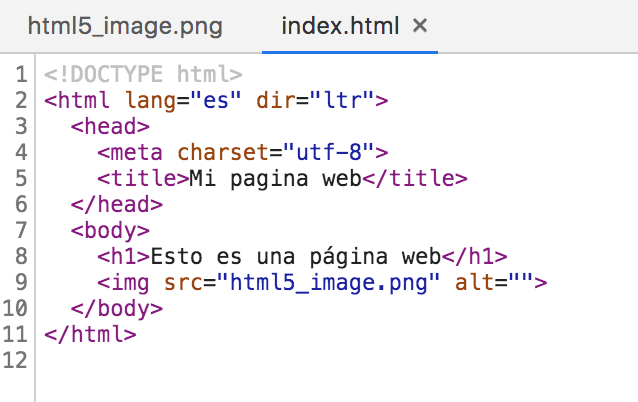
\includegraphics[width=0.9\textwidth, height=0.5\textwidth]{chapters/images/simplehtmlpage.png}
    \caption{Fuente de la página web}
    \label{fig:f2}
  \end{subfigure}
  \begin{subfigure}[b]{0.5\textwidth}
  \centering
    
\includegraphics[width=0.9\textwidth, height=0.5\textwidth]{chapters/images/simplehtml.png}
    \caption{Página web visualización}
    \label{fig:f1}
  \end{subfigure}
  \hfill
  
  \caption{Ejemplo de página web con HTML5}
\end{figure}

Generalmente junto con HTML se utilizan otras dos tecnologías web: CSS para la apariencia/presentación y JavaScript para la funcionalidad/comportamiento de una página web.
\\
\\
Kibotics utiliza plantillas basadas en HTML5 en las páginas web que sirve. En este TFG se va a utilizar HTML5 para modificar y crear las plantillas de las páginas web que mostrarán los nuevos ejercicios que vamos a introducir en la plataforma.

\subsection{JavaScript}
JavaScript es un lenguaje de programación interpretado, no necesita compilar los programas para ejecutarlos, pero sí un intérprete que en nuestro caso es el navegador. JavaScript sigue el estándar ECMAScript que se encarga de regir cómo debe ser interpretado, su operatividad y buen funcionamiento. Este lenguaje posee una sintaxis derivada de C y Java pero no tiene nada que ver con ellos.

Se utiliza principalmente para crear páginas web interactivas, que incorporan efectos como texto que aparece y
desaparece, animaciones, acciones que se activan al pulsar botones y ventanas con
mensajes de aviso al usuario\cite{javascript}.

El código JavaScript se ejecuta en el navegador del cliente y permite que éste interactúe con la página web. En la siguiente Figura 3.2 podemos ver un ejemplo de página web interactiva.\footnote{https://martaquintana.github.io/2018-19-CSAAI-Pong/pong-01.html}

\begin{figure}[H]
  \begin{subfigure}[b]{0.5\textwidth}
  \centering
    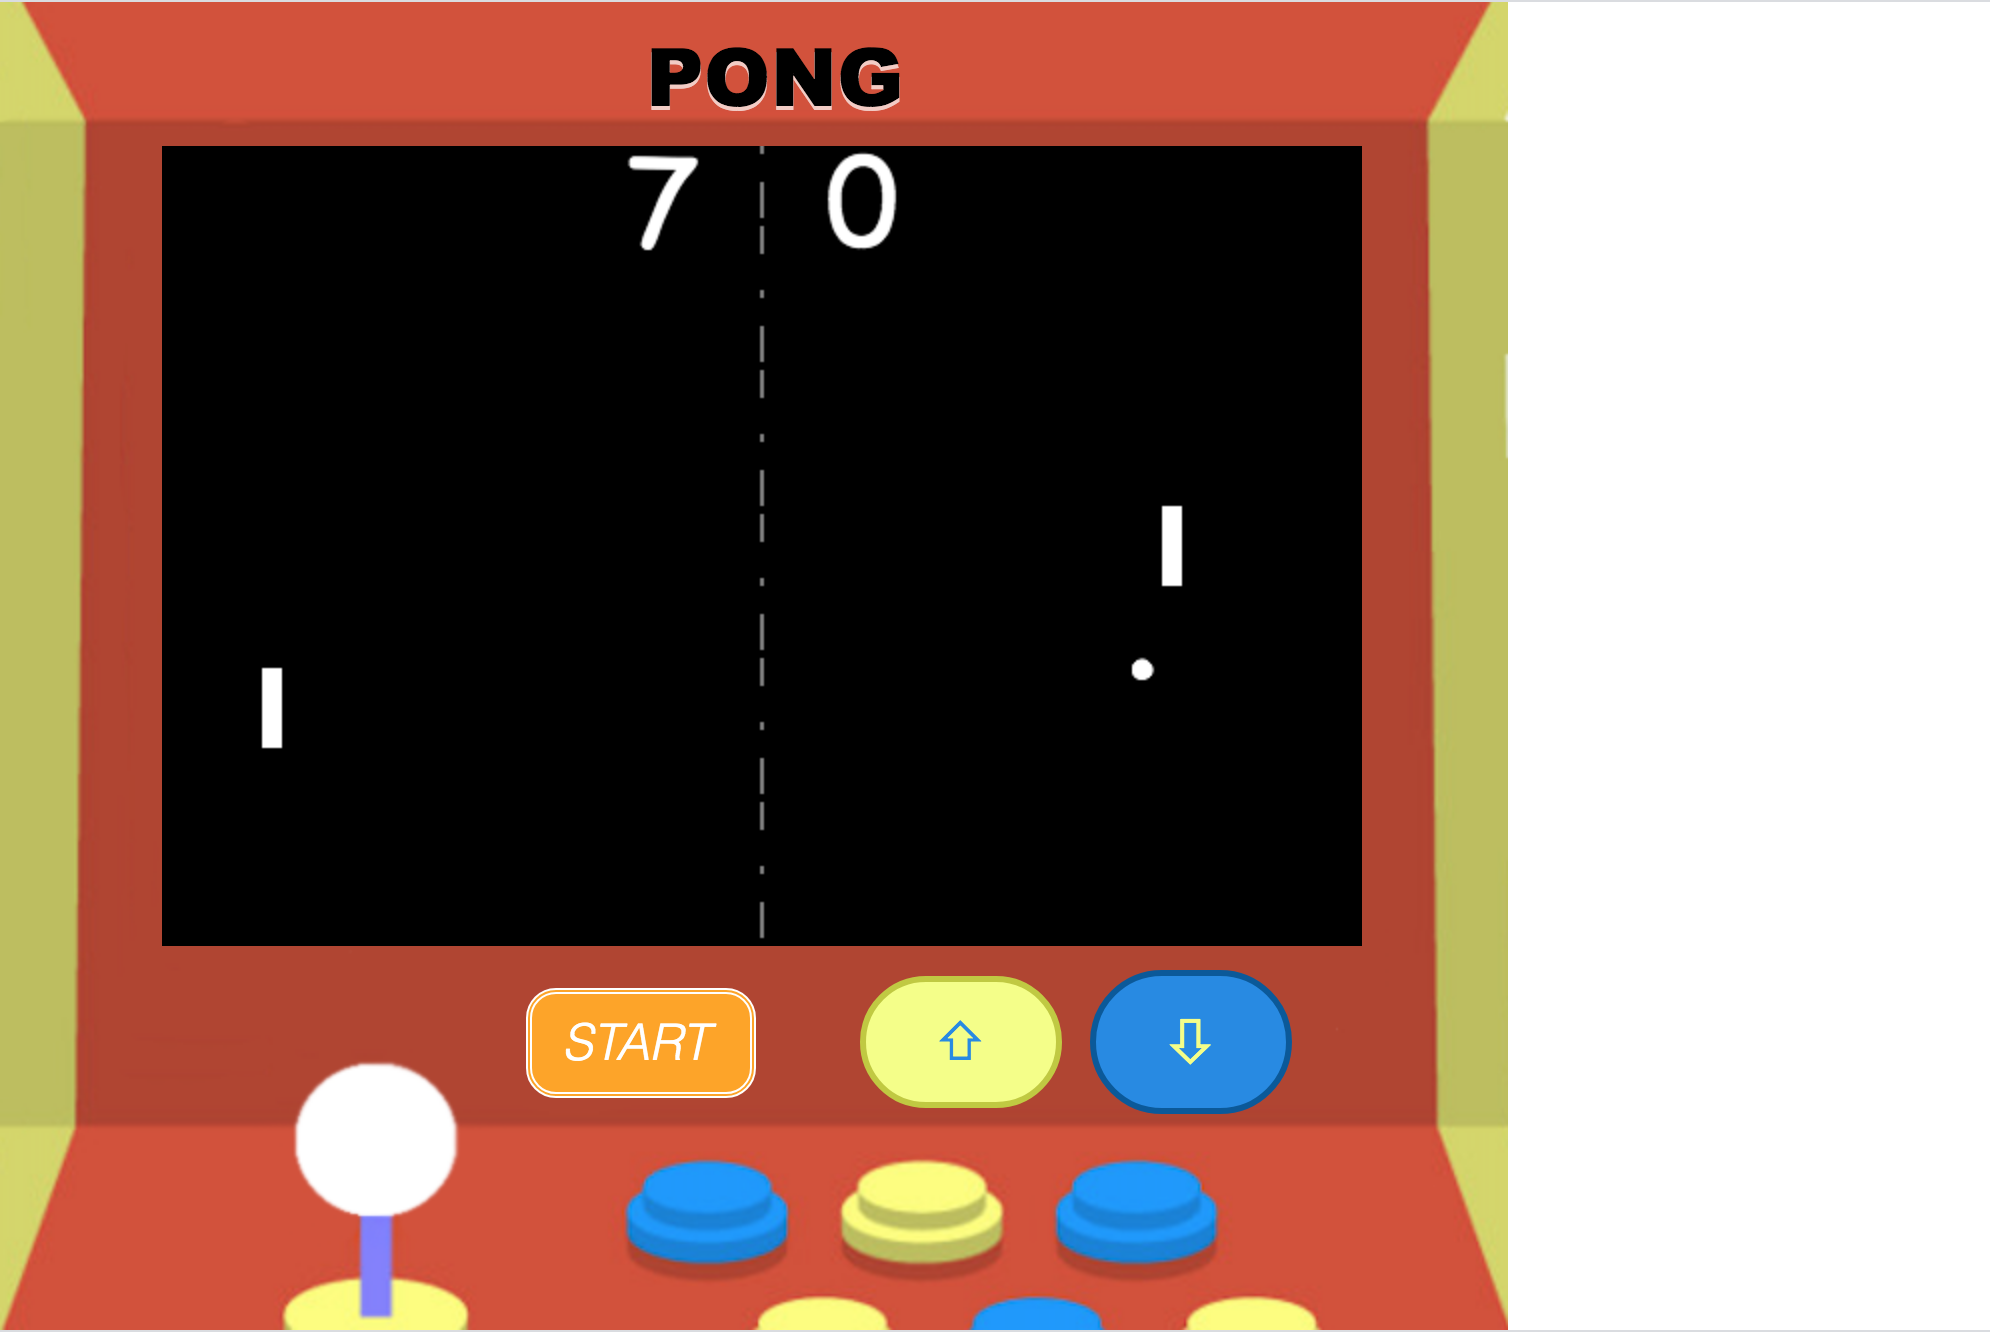
\includegraphics[width=1\textwidth, height=0.6\textwidth]{chapters/images/pong.png}
    \caption{Página web visualización}
    \label{fig:f1}
  \end{subfigure}
  \hfill
  \begin{subfigure}[b]{0.5\textwidth}
  \centering
    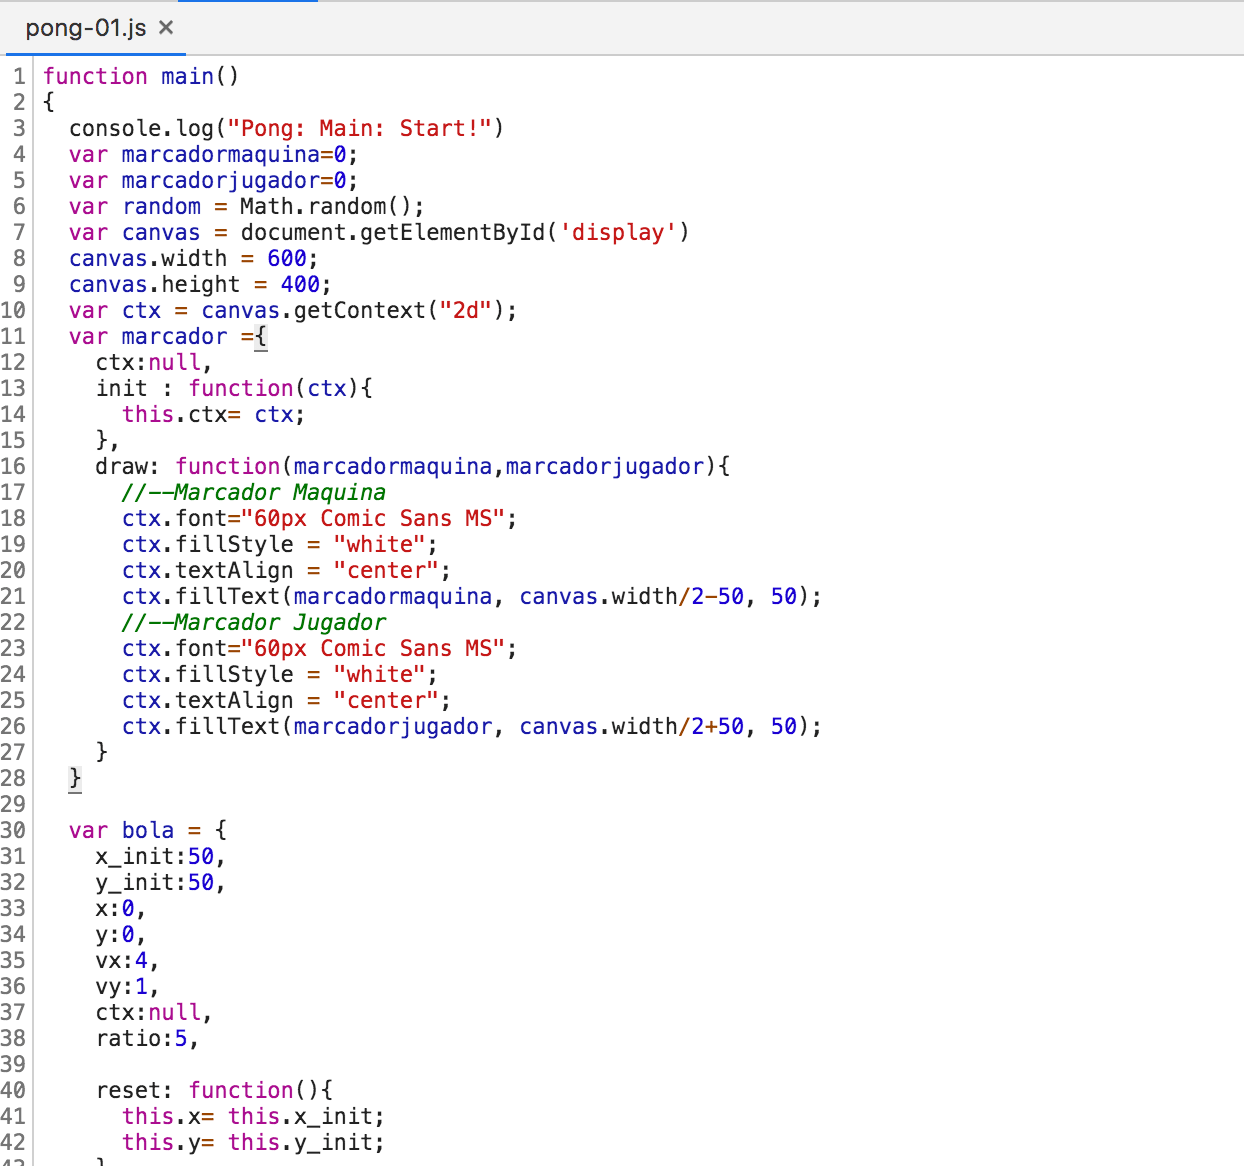
\includegraphics[width=1\textwidth, height=0.6\textwidth]{chapters/images/codigojs.png}
    \caption{Código JavaScript}
    \label{fig:f2}
  \end{subfigure}
  \caption{Ejemplo de página web interactiva con HTML5, CSS3 y JavaScript }
\end{figure}

En este trabajo JavaScript ha sido una pieza clave para su desarrollo y todos los ejercicios se han creado usando este lenguaje de programación.
 
\subsection{Python y Scratch}

Python es un lenguaje de programación orientado a objetos, es un lenguaje interpretado o de script, y al igual que JavaScript necesita un programa intermedio que haga de ``intérprete''. Es un lenguaje fuertemente tipado y multiplataforma. Su filosofía es que el código sea legible y tenga  una sintaxis muy limpia. Sencillo pero potente, lenguaje muy usado en la universidad y trabajo \cite{python}.

El servidor de Kibotics está programado en Python (usa la tecnología web Django). Los ejercicios disponibles en la plataforma se pueden resolver también con este lenguaje. Para usar Python las páginas web de los ejercicios contienen el editor ACE. ACE es un editor de código incrustable escrito en JavaScript \cite{aceeditor}. Esto permite al usuario escribir el código de la solución del ejercicio en Python e internamente este código se traduce a JavaScript para el correcto funcionamiento de los ejercicios. 

Como hemos comentado en la introducción, Scratch es un lenguaje de programación visual basado en bloques, creado y mantenido por Lifelong Kindergarten group en el MIT Media Lab. Para usar Scratch en Kibotics se usa Blocky, que es una librería de JavaScript desarrollada por Google. Permite usar en una página web un editor de código visual. Es compatible con Chrome, Firefox, Safari, Opera y otros navegadores. Corresponde a tecnologías del lado cliente y no tiene dependencia con el servidor \cite{blocky}.


Los ejercicios planteados en este TFG están resueltos tanto en Python como en Scratch. Al ser una plataforma para el ámbito educativo estos dos lenguajes son una buena alternativa para empezar a programar porque son lenguajes sencillos y con una curva de aprendizaje muy suave. En la Figura 3.3 podemos ver unos ejemplos de soluciones.

\begin{figure}[H]
  \begin{subfigure}[b]{1\textwidth}
  \centering
    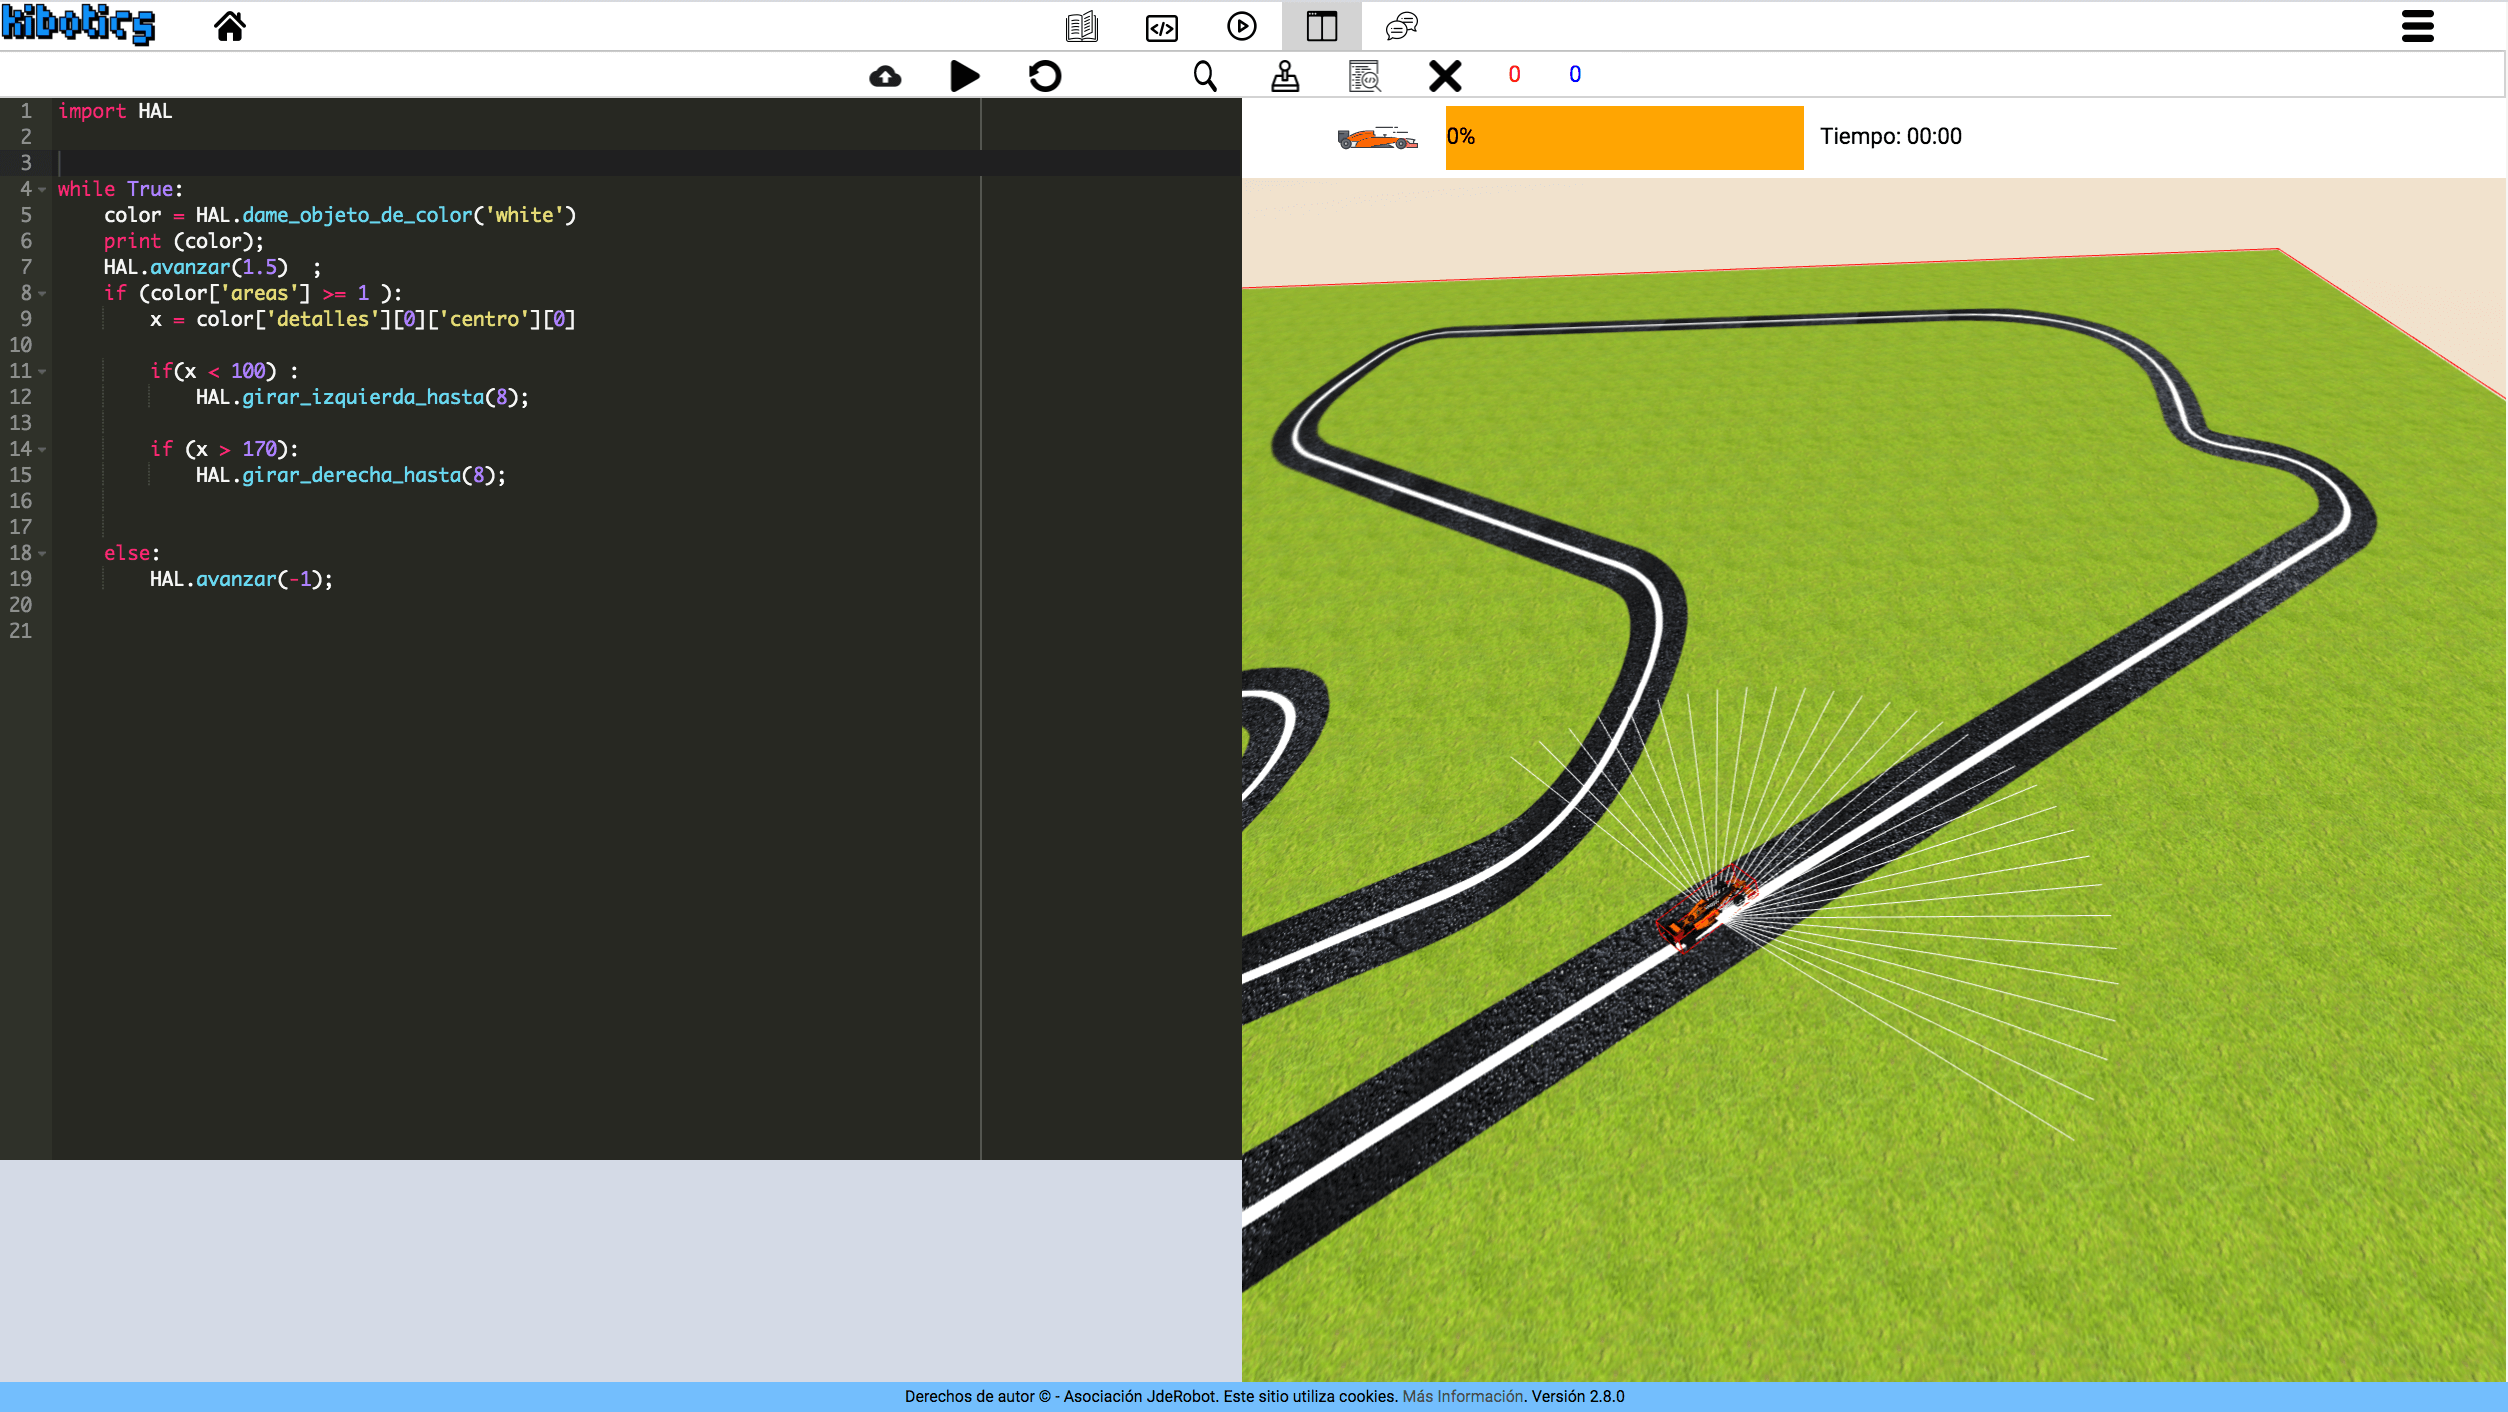
\includegraphics[width=0.95\textwidth, height=0.4\textwidth]{chapters/images/python.png}
    \caption{Solución en Python}
    \label{fig:f1}
  \end{subfigure}
  \hfill
  \begin{subfigure}[b]{1\textwidth}
  \centering
    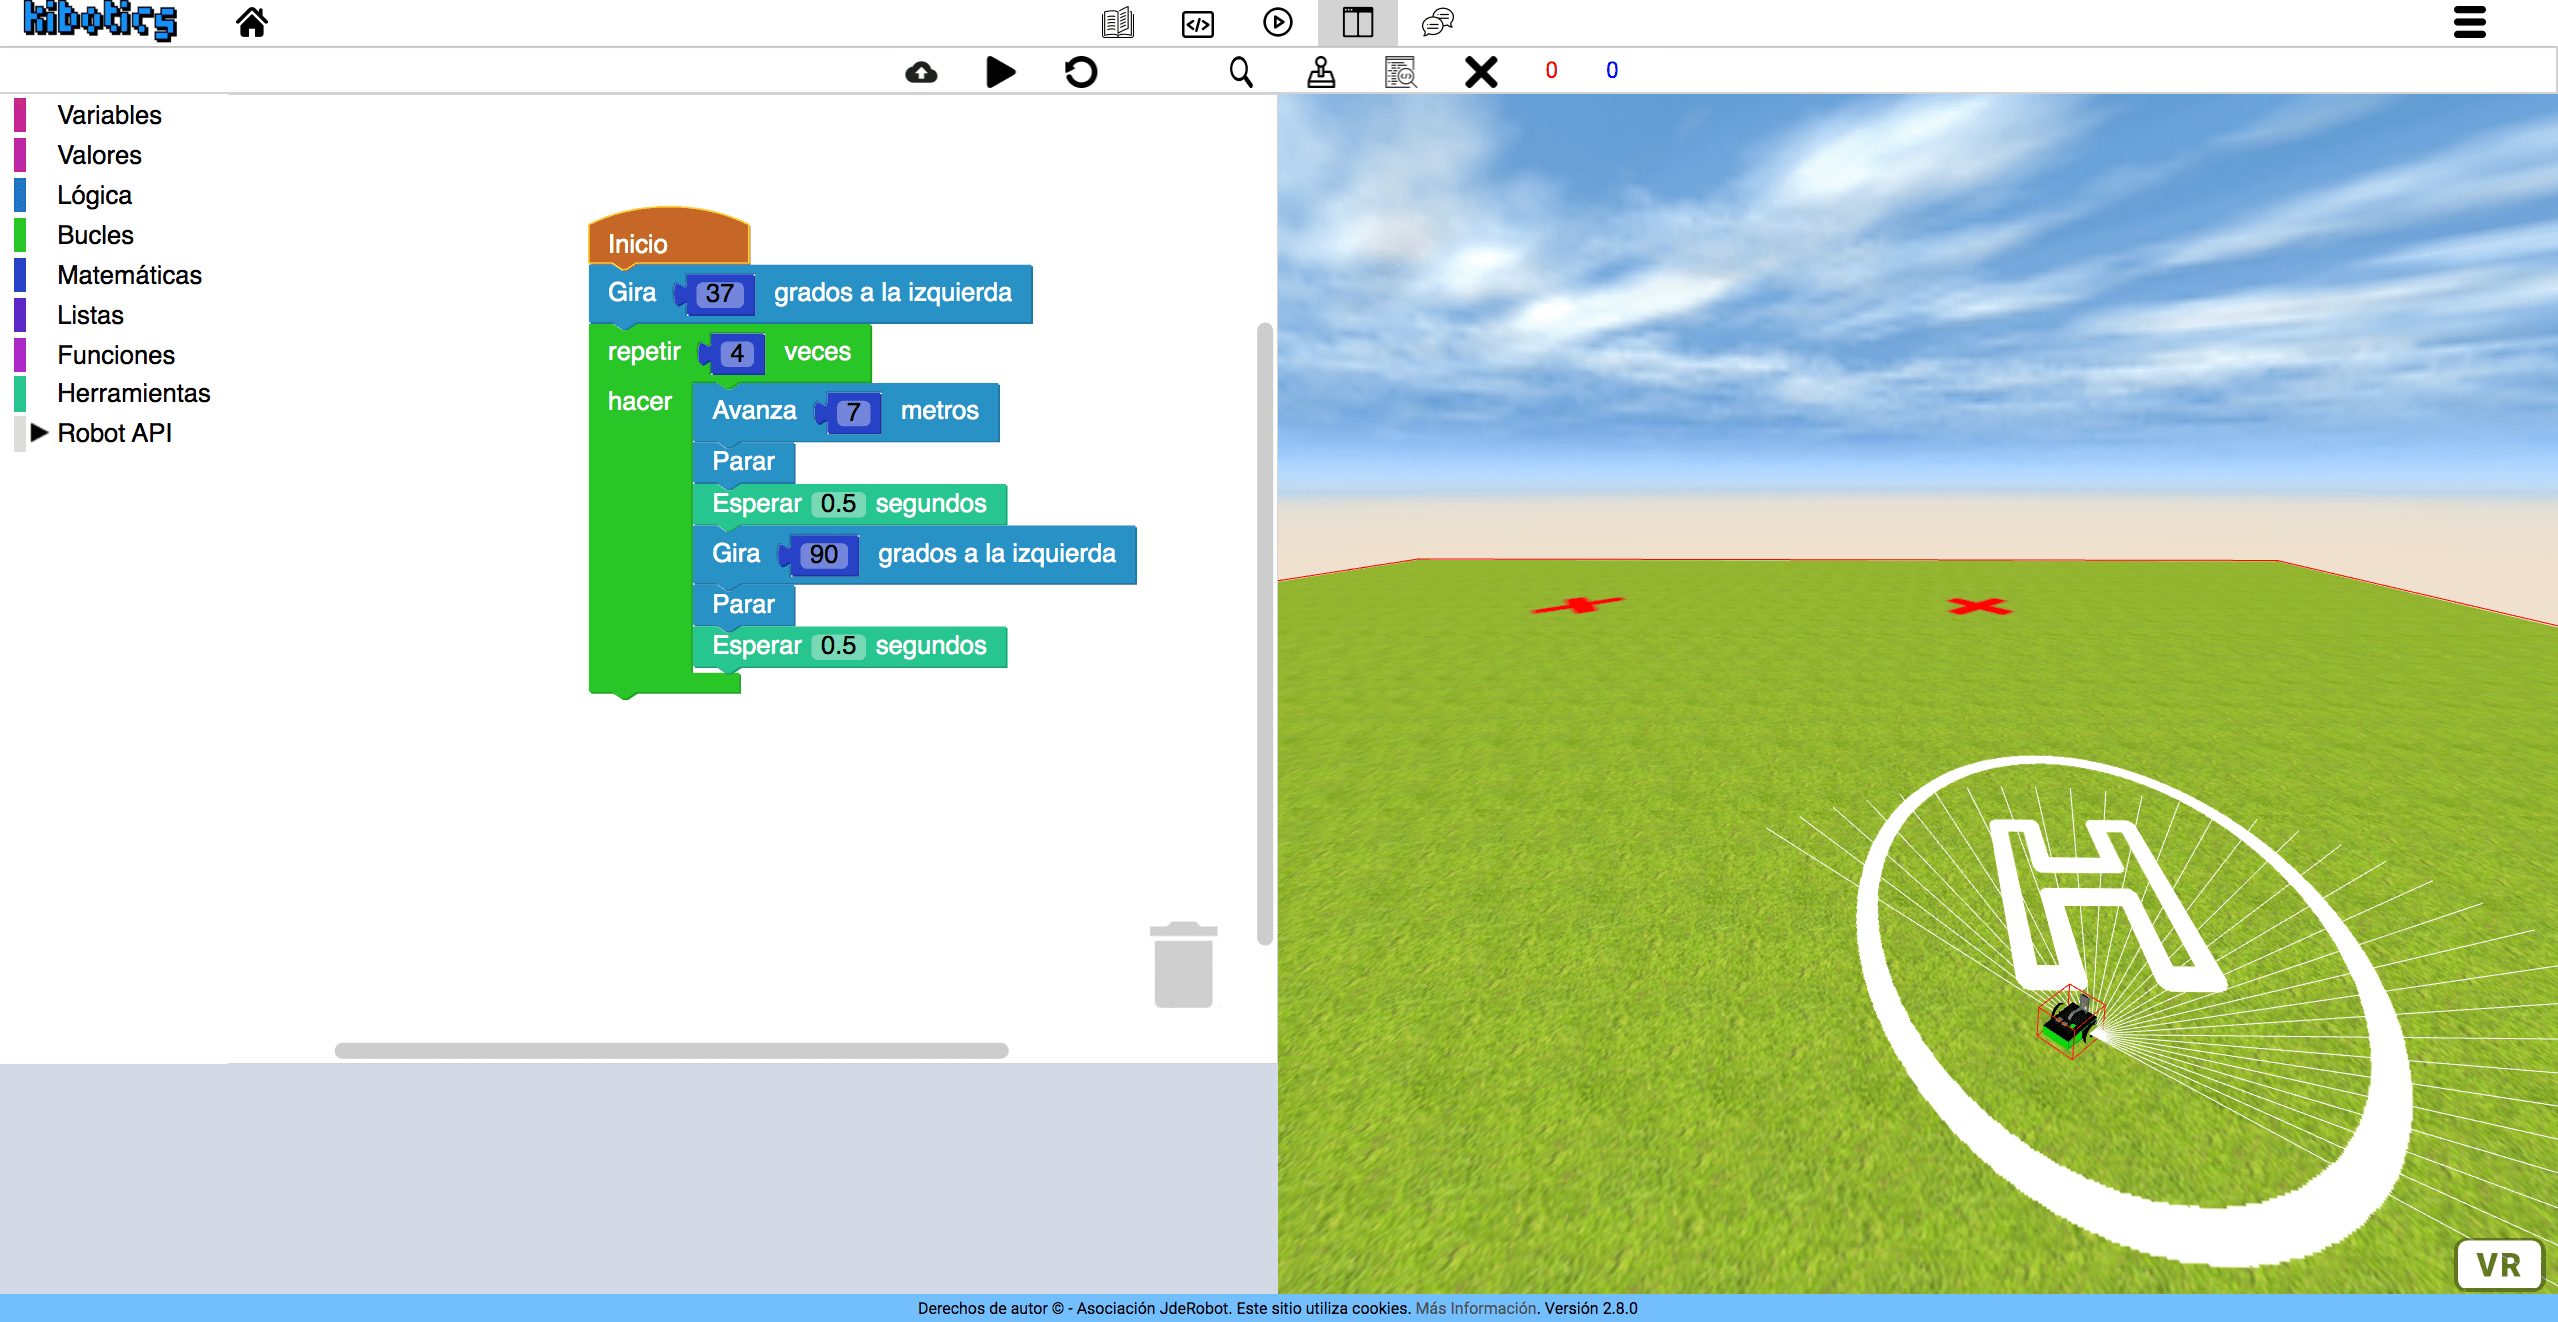
\includegraphics[width=0.95\textwidth, height=0.4\textwidth]{chapters/images/scratch2.png}
    \caption{Solución en Scratch}
    \label{fig:f2}
  \end{subfigure}
  \caption{Ejemplo de código en Kibotics }
\end{figure}


\subsection{JSON} JSON, cuyas siglas significan JavaScript Object Notation, es un formato de intercambio de datos muy ligero. Para nosotros es fácil de leer y escribir, además la interpretación y generación de ficheros es muy sencilla para las máquinas \cite{json}.

JSON es un formato de datos basado en texto estándar para representar datos estructurados con la sintaxis de objetos de JavaScript. Son archivos de texto plano con codificación UTF8, que son compatibles con todos los sistemas. Se utiliza para transmitir datos en aplicaciones web \cite{json2}. 
Este formato puede ser utilizado independientemente de JavaScript, y muchos entornos de programación poseen la capacidad de leer (convertir; \textit{parsear}) y generar ficheros JSON. En nuestro caso vamos a leer ficheros JSON desde JavaScript.

Un fichero JSON  típicamente está compuesto de dos estructuras: 
\begin{itemize}
    \item \textbf{Una colección de pares de nombre/valor}: En otros lenguajes son conocidos como objeto, registro, estructura, diccionario o lista de claves. 
    Ejemplo objeto: 
    \begin{lstlisting}
    {
        "id" : 7,
        "name" : "Robot",
        "type" : "Drone"
    }
     \end{lstlisting}
    \item \textbf{Una lista ordenada de valores}: En la mayoría de los lenguajes, esto se implementa como arreglos \textit{arrays}, vectores o listas.  
     Ejemplo array:  
     \begin{lstlisting}
        [ "blue", "yellow", "orange" ]
     \end{lstlisting}
\end{itemize}

Estas estructuras son universales en todos los lenguajes de programación, es por esto que  JSON es muy fácil utilizar para un programador. Todos los lenguajes disponen de funciones para interpretar cadenas JSON y convertir datos en cadenas JSON válidas.

En la Figura 3.4 podemos ver una pequeña parte de un fichero de configuración de un ejercicio con JSON en Kibotics. En esta plataforma se utiliza JSON para crear los ejercicios con las características específicas que le correspondan y en este TFG se han usado tanto para la creación de los mundos como para fijar las posiciones de los confetis en el ejercicio del Roomba que veremos más adelante.

\begin{figure}[H]
    \centering
    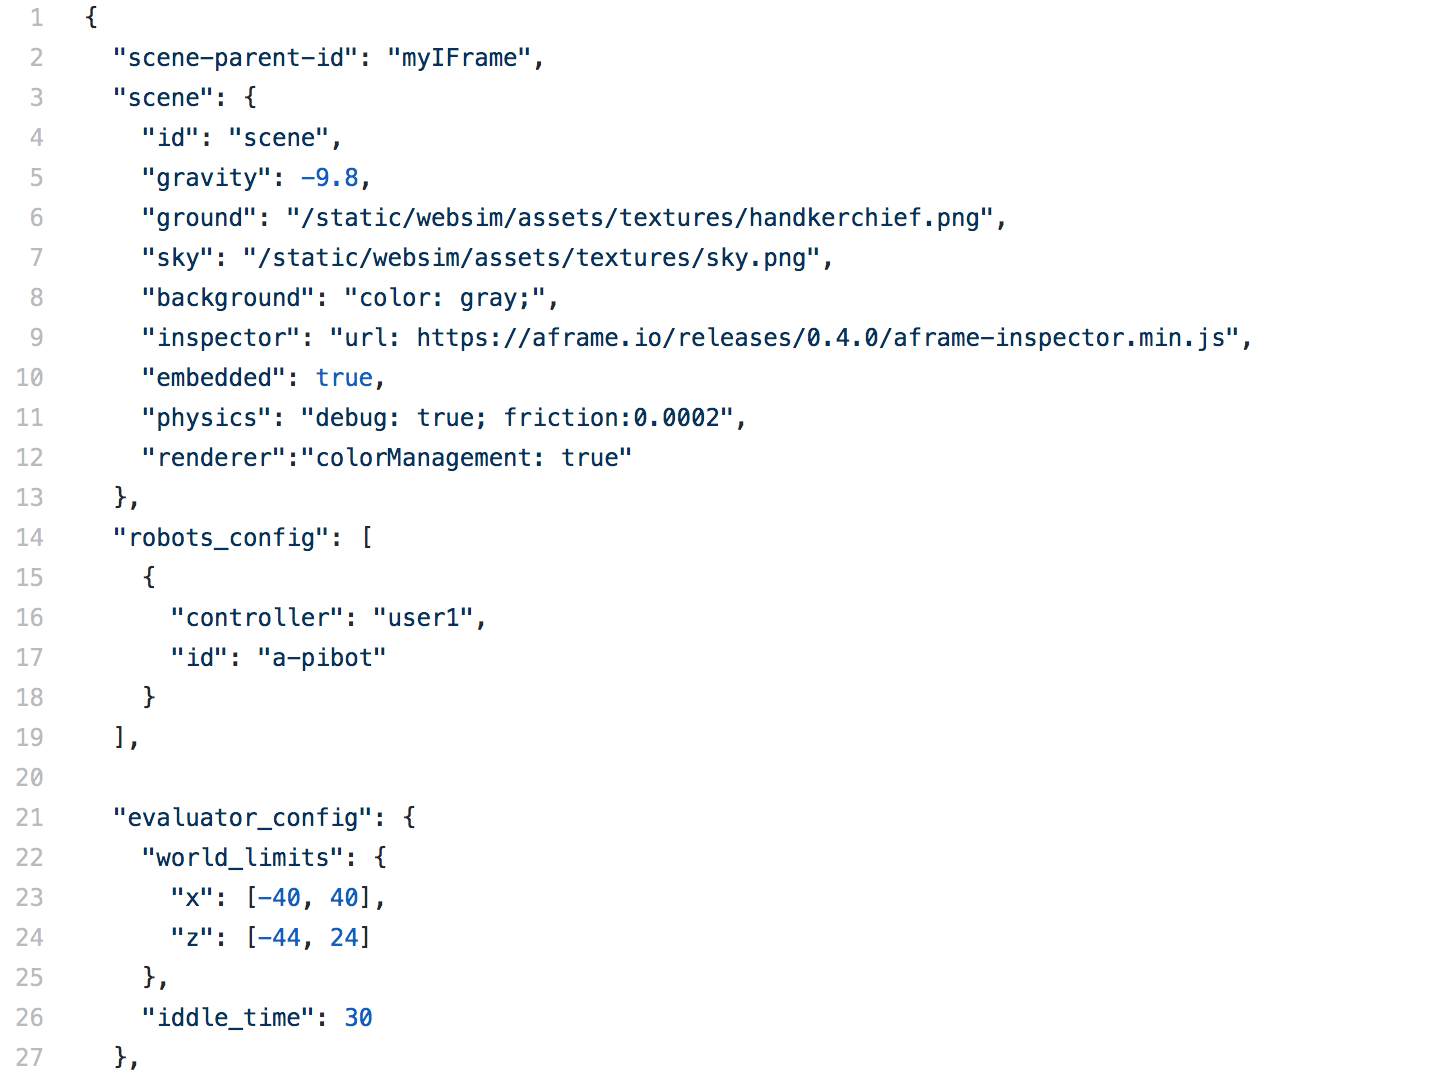
\includegraphics[width=0.6\textwidth, height=0.4\textwidth]{chapters/images/json.png}
    \caption{Parte de un fichero config.json de un ejercicio en Kibotics}
    \label{fig:my_label}
\end{figure}

\section{Herramientas}
\subsection{TensorFlowJS, Web Audio API y Teachable Machine}
Para procesar el audio en JavaScript se han tenido que analizar diferentes herramientas o APIs\footnote{Interfaz de programación de aplicaciones} de procesamiento de audio en la web. De esta forma hemos podido elegir la herramienta que mejor se adapta a nuestro problema.
Entre ellas TensorFlowJS, Web Audio API y Teachable Machine (Figura 3.5) son las herramientas que se han estudiado para llevar a cabo el teleoperador acústico.
\\
TensorFlowJS es una biblioteca de JavaScript para el entrenamiento y la implementación de modelos de aprendizaje automático en navegadores y en Node.js . TensorFlow es una plataforma de código abierto para la creación de modelos de aprendizaje automático \cite{tfjs}.

La API de Audio Web provee un sistema poderoso y versatil para controlar audio en la Web, permitiendo a los desarrolladores escoger fuentes de audio, agregar efectos al audio, crear visualizaciones de audios y aplicar efectos espaciales, entre otras cosas \cite{waa}.

Teachable Machine es una herramienta basada en la Web que hace posible crear modelos de aprendizaje automático de manera rápida, sencilla y accesible para todos \cite{tm}.

\begin{figure}[H]
    \centering
    \begin{subfigure}{.3\linewidth}
        
\includegraphics[width=1\textwidth]{chapters/images/tfjs.png}
        \caption{Tensor Flow JS}
    \end{subfigure}
    \hskip2em
    \begin{subfigure}{.3\linewidth}
    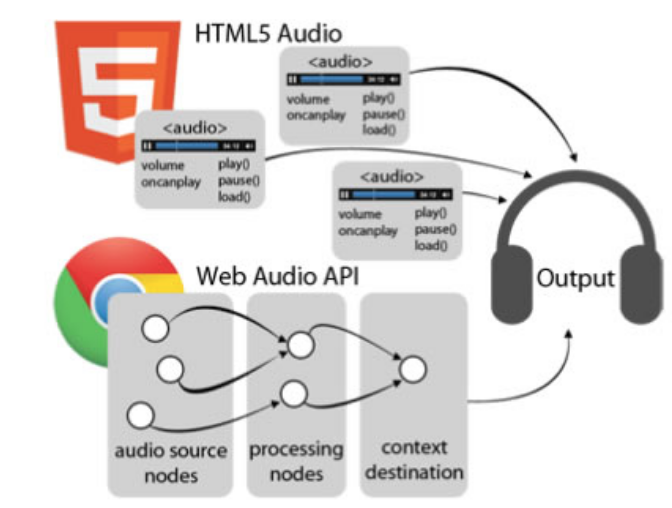
\includegraphics[width=1\textwidth]{chapters/images/waa.png}
        \caption{Web Audio API}
    \end{subfigure}
    \begin{subfigure}{.3\linewidth}
       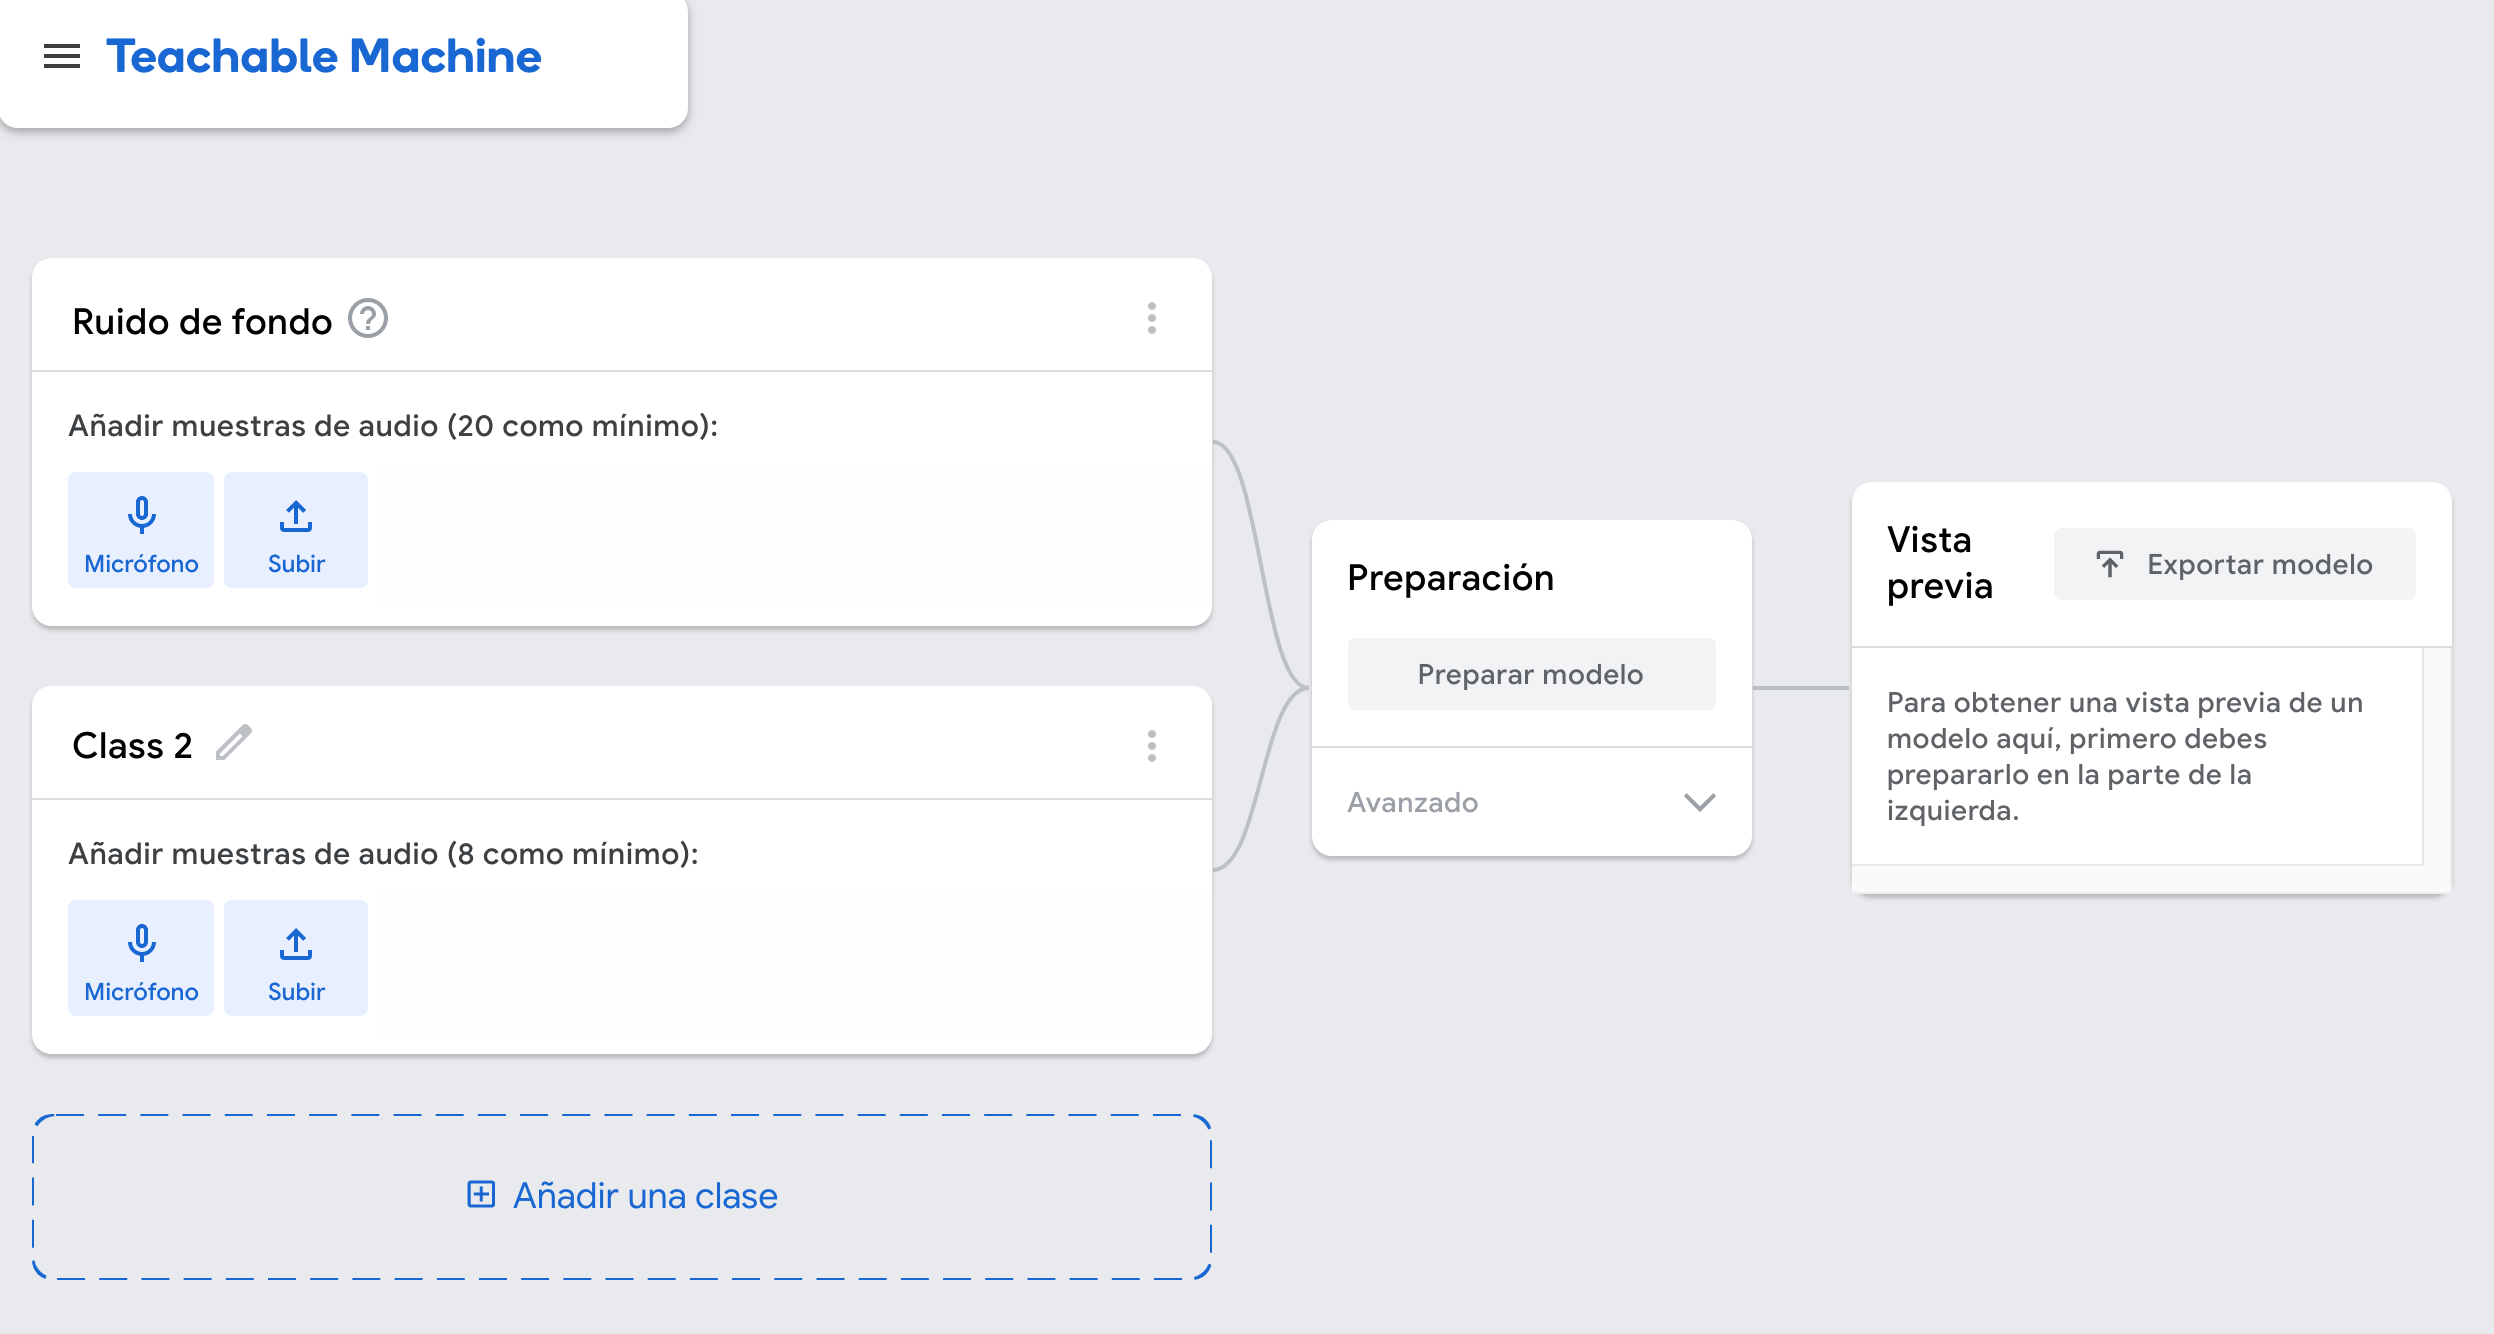
\includegraphics[width=1\textwidth, height=0.7\textwidth]{chapters/images/tm.png}
        \caption{Teachable Machine}
    \end{subfigure}
    \caption{Herramientas de reconocimiento de audio}
\end{figure}


En el Capítulo 4 se explicará en profundidad cómo se han usado estas tecnologías y por qué después de probar con cada una de estas tres herramientas, hemos elegido Teachable Machine para el desarrollo final del Teleoperador Acústico.


\subsection{A-Frame}

A-Frame es un marco web para crear experiencias de realidad virtual (VR). A-Frame utiliza HTML declarativo, lo que facilita bastante la creación de escenas en 3D y es accesible para todos, desde desarrolladores web, artistas y diseñadores, a educadores y estudiantes. Su estructura entidad-componente proporciona una infinidad de posibilidades y ofrece compatibilidad con \textit{three.js}, una biblioteca  escrita en JavaScript para crear y mostrar gráficos animados 3D en un navegador Web. 

Sin instalar nada, A-Frame permite manejar modelos 3D para crear entornos de realidad virtual solamente usando las etiquetas \textless script\textgreater  y \textless a-scene\textgreater. Es compatible con aplicaciones de realidad virtual como GearVR y Windows Mixed Reality entre otras. Además funciona perfectamente en ordenadores y teléfonos inteligentes \cite{aframe}. 


Para crear escenas en una página web solo es necesario importar la librería de A-Frame de esta forma: \begin{lstlisting}
    <script src="https://aframe.io/releases/1.2.0/aframe.min.js"></script>
\end{lstlisting} 
y poner las etiquetas corresponientes a-scene y los objetos que queramos que aparezacan en la escena con sus atributos.
A continuación se muestra un ejemplo de código correspondiente con la visualización de la escena en el navegador en la Figura 3.6.
\\
\begin{lstlisting}
    <html>
      <head>
        <script src="https://aframe.io/releases/1.2.0/aframe.min.js"></script>
      </head>
      <body>
        <a-scene>
          <a-box position="-1 0.5 -3" rotation="0 45 0" color="#4CC3D9"></a-box>
          <a-sphere position="0 1.25 -5" radius="1.25" color="#EF2D5E"></a-sphere>
          <a-cylinder position="1 0.75 -3" radius="0.5" height="1.5" color="#FFC65D"></a-cylinder>
          <a-plane position="0 0 -4" rotation="-90 0 0" width="4" height="4" color="#7BC8A4"></a-plane>
          <a-sky color="#ECECEC"></a-sky>
        </a-scene>
      </body>
    </html>
\end{lstlisting}

\begin{figure}[H]
    \centering
    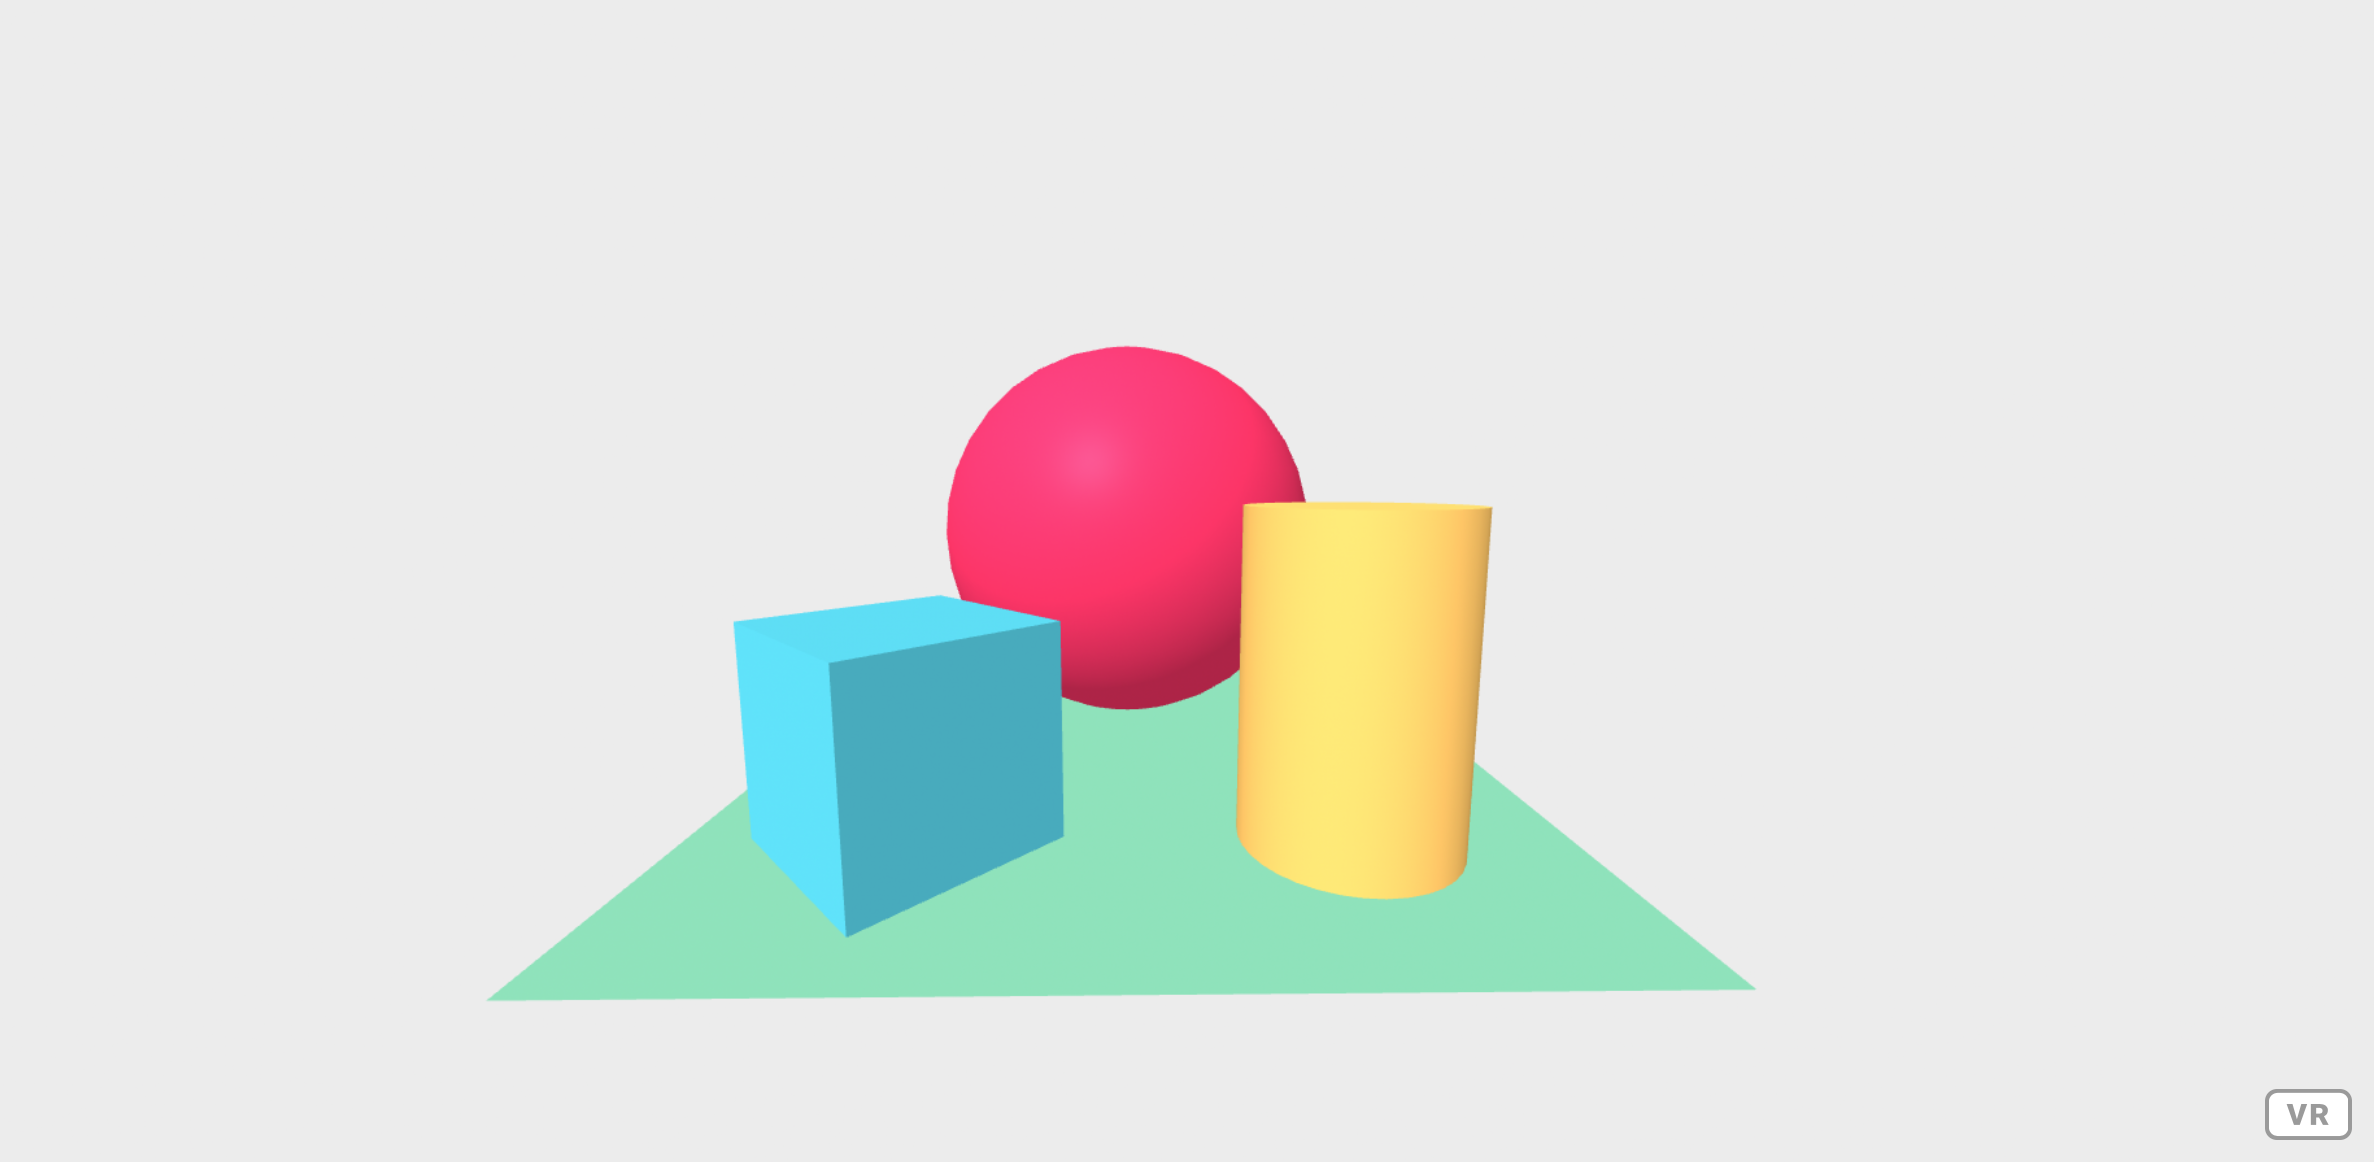
\includegraphics[width=1\textwidth, height=0.5\textwidth]{chapters/images/aframe.png}
    \caption{Ejemplo escena en A-Frame}
    \label{fig:my_label}
\end{figure}

A-Frame proporciona un inspector visual 3D incorporado (Figura 3.7). Presionando ctrl + alt + i, podemos inspeccionar la escena, esto es muy útil cuando necesitas la posición concreta de un objeto.

\begin{figure}[H]
    \centering
    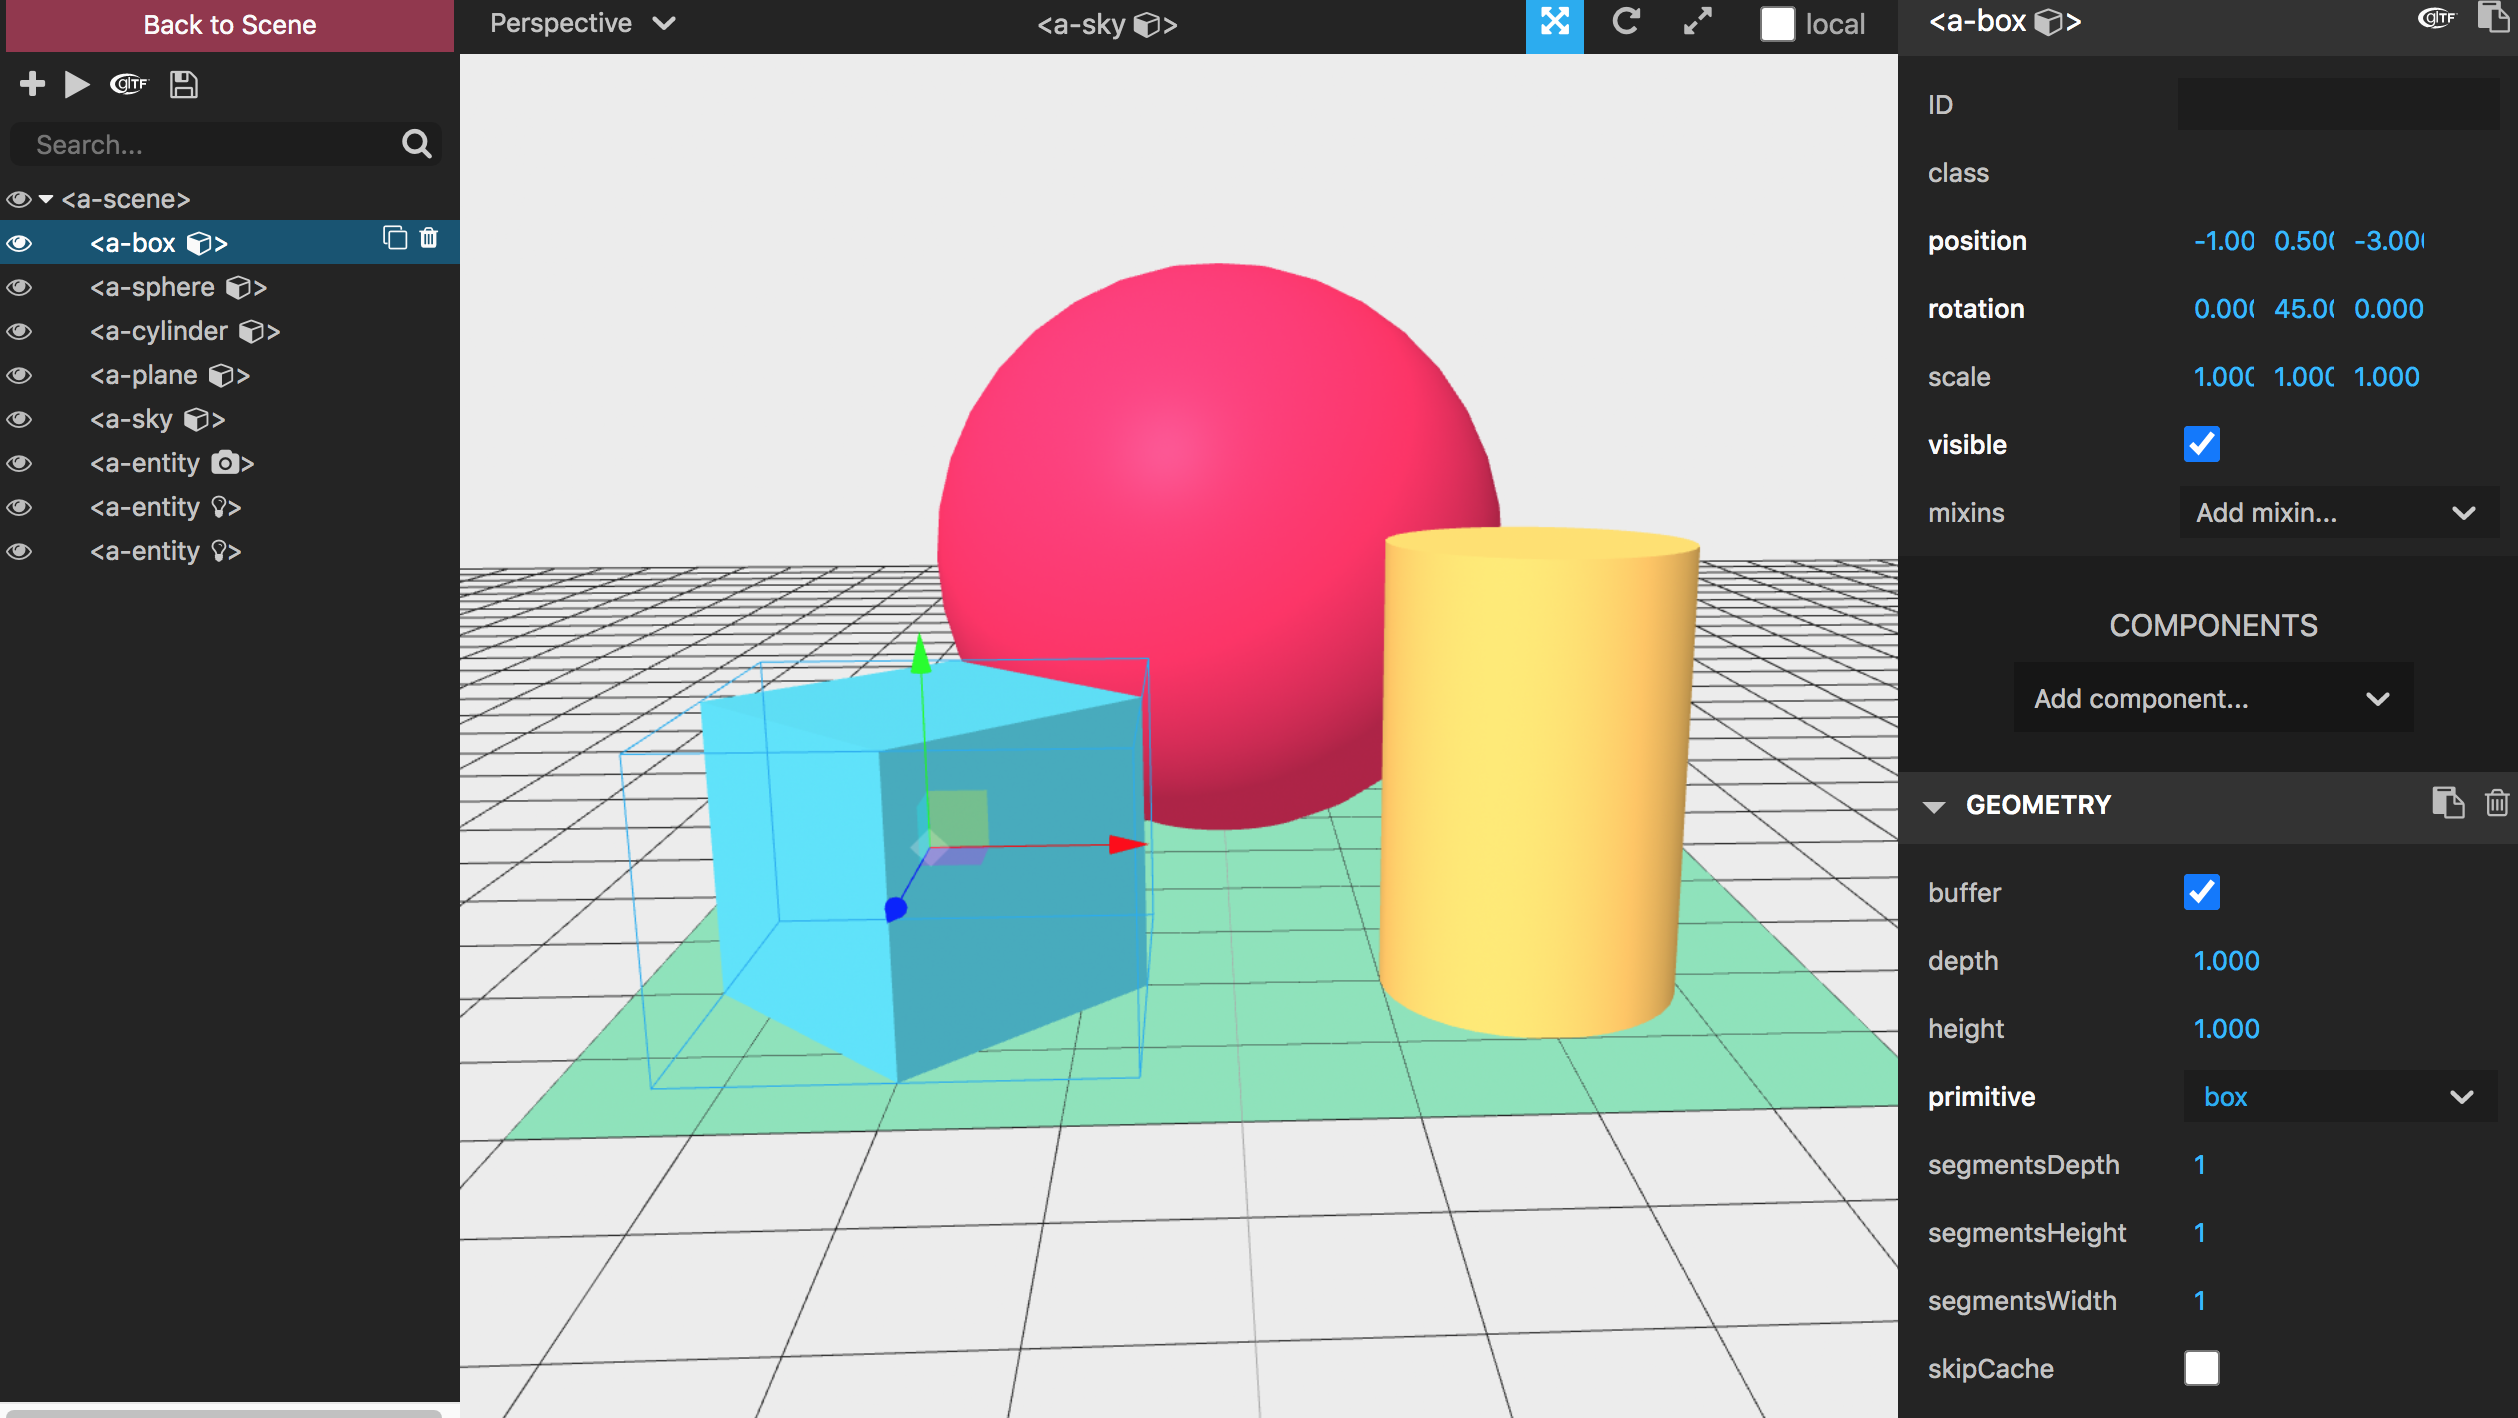
\includegraphics[width=0.8\textwidth, height=0.5\textwidth]{chapters/images/inspectoraframe.png}
    \caption{Inspector en A-Frame}
    \label{fig:my_label}
\end{figure}


En nuestro caso \textit{a-entity} serán los modelos 3D de los robots que se crearán con Blender  y se usarán componentes como \textit{a-box}, \textit{a-plane}, \textit{a-cylinder} y \textit{a-sphere} para crear componentes adicionales a la escena dándoles sus respectivas texturas. En este trabajo se ha usado la versión 1.1.0 de A-Frame.

\subsection{Blender}
Blender es un software de creación de modelos 3D gratuito, de código abierto y multiplataforma. Este programa se utiliza para el modelado, montaje, animación, simulación, renderizado 3d, así como para la  composición y seguimiento de movimiento, edición de vídeo y animación 2D
\cite{blender}. En este trabajo se ha usado la versión 2.93.0 de Blender.

Para exportar los modelos de Blender se ha usado el formato glTF (GL Transmission Format). Es un formato de archivo para escenas y modelos 3D basado en JSON. De esta forma se pueden integrar los modelos en A-Frame de forma sencilla y rápida.

Este programa se ha utilizado en este proyecto para crear los nuevos robots, escenarios e introducir animaciones a la plataforma. En la Figura 3.8 se muestra un ejemplo de un cubo animado con Blender. 

\begin{figure}[H]
    \centering
    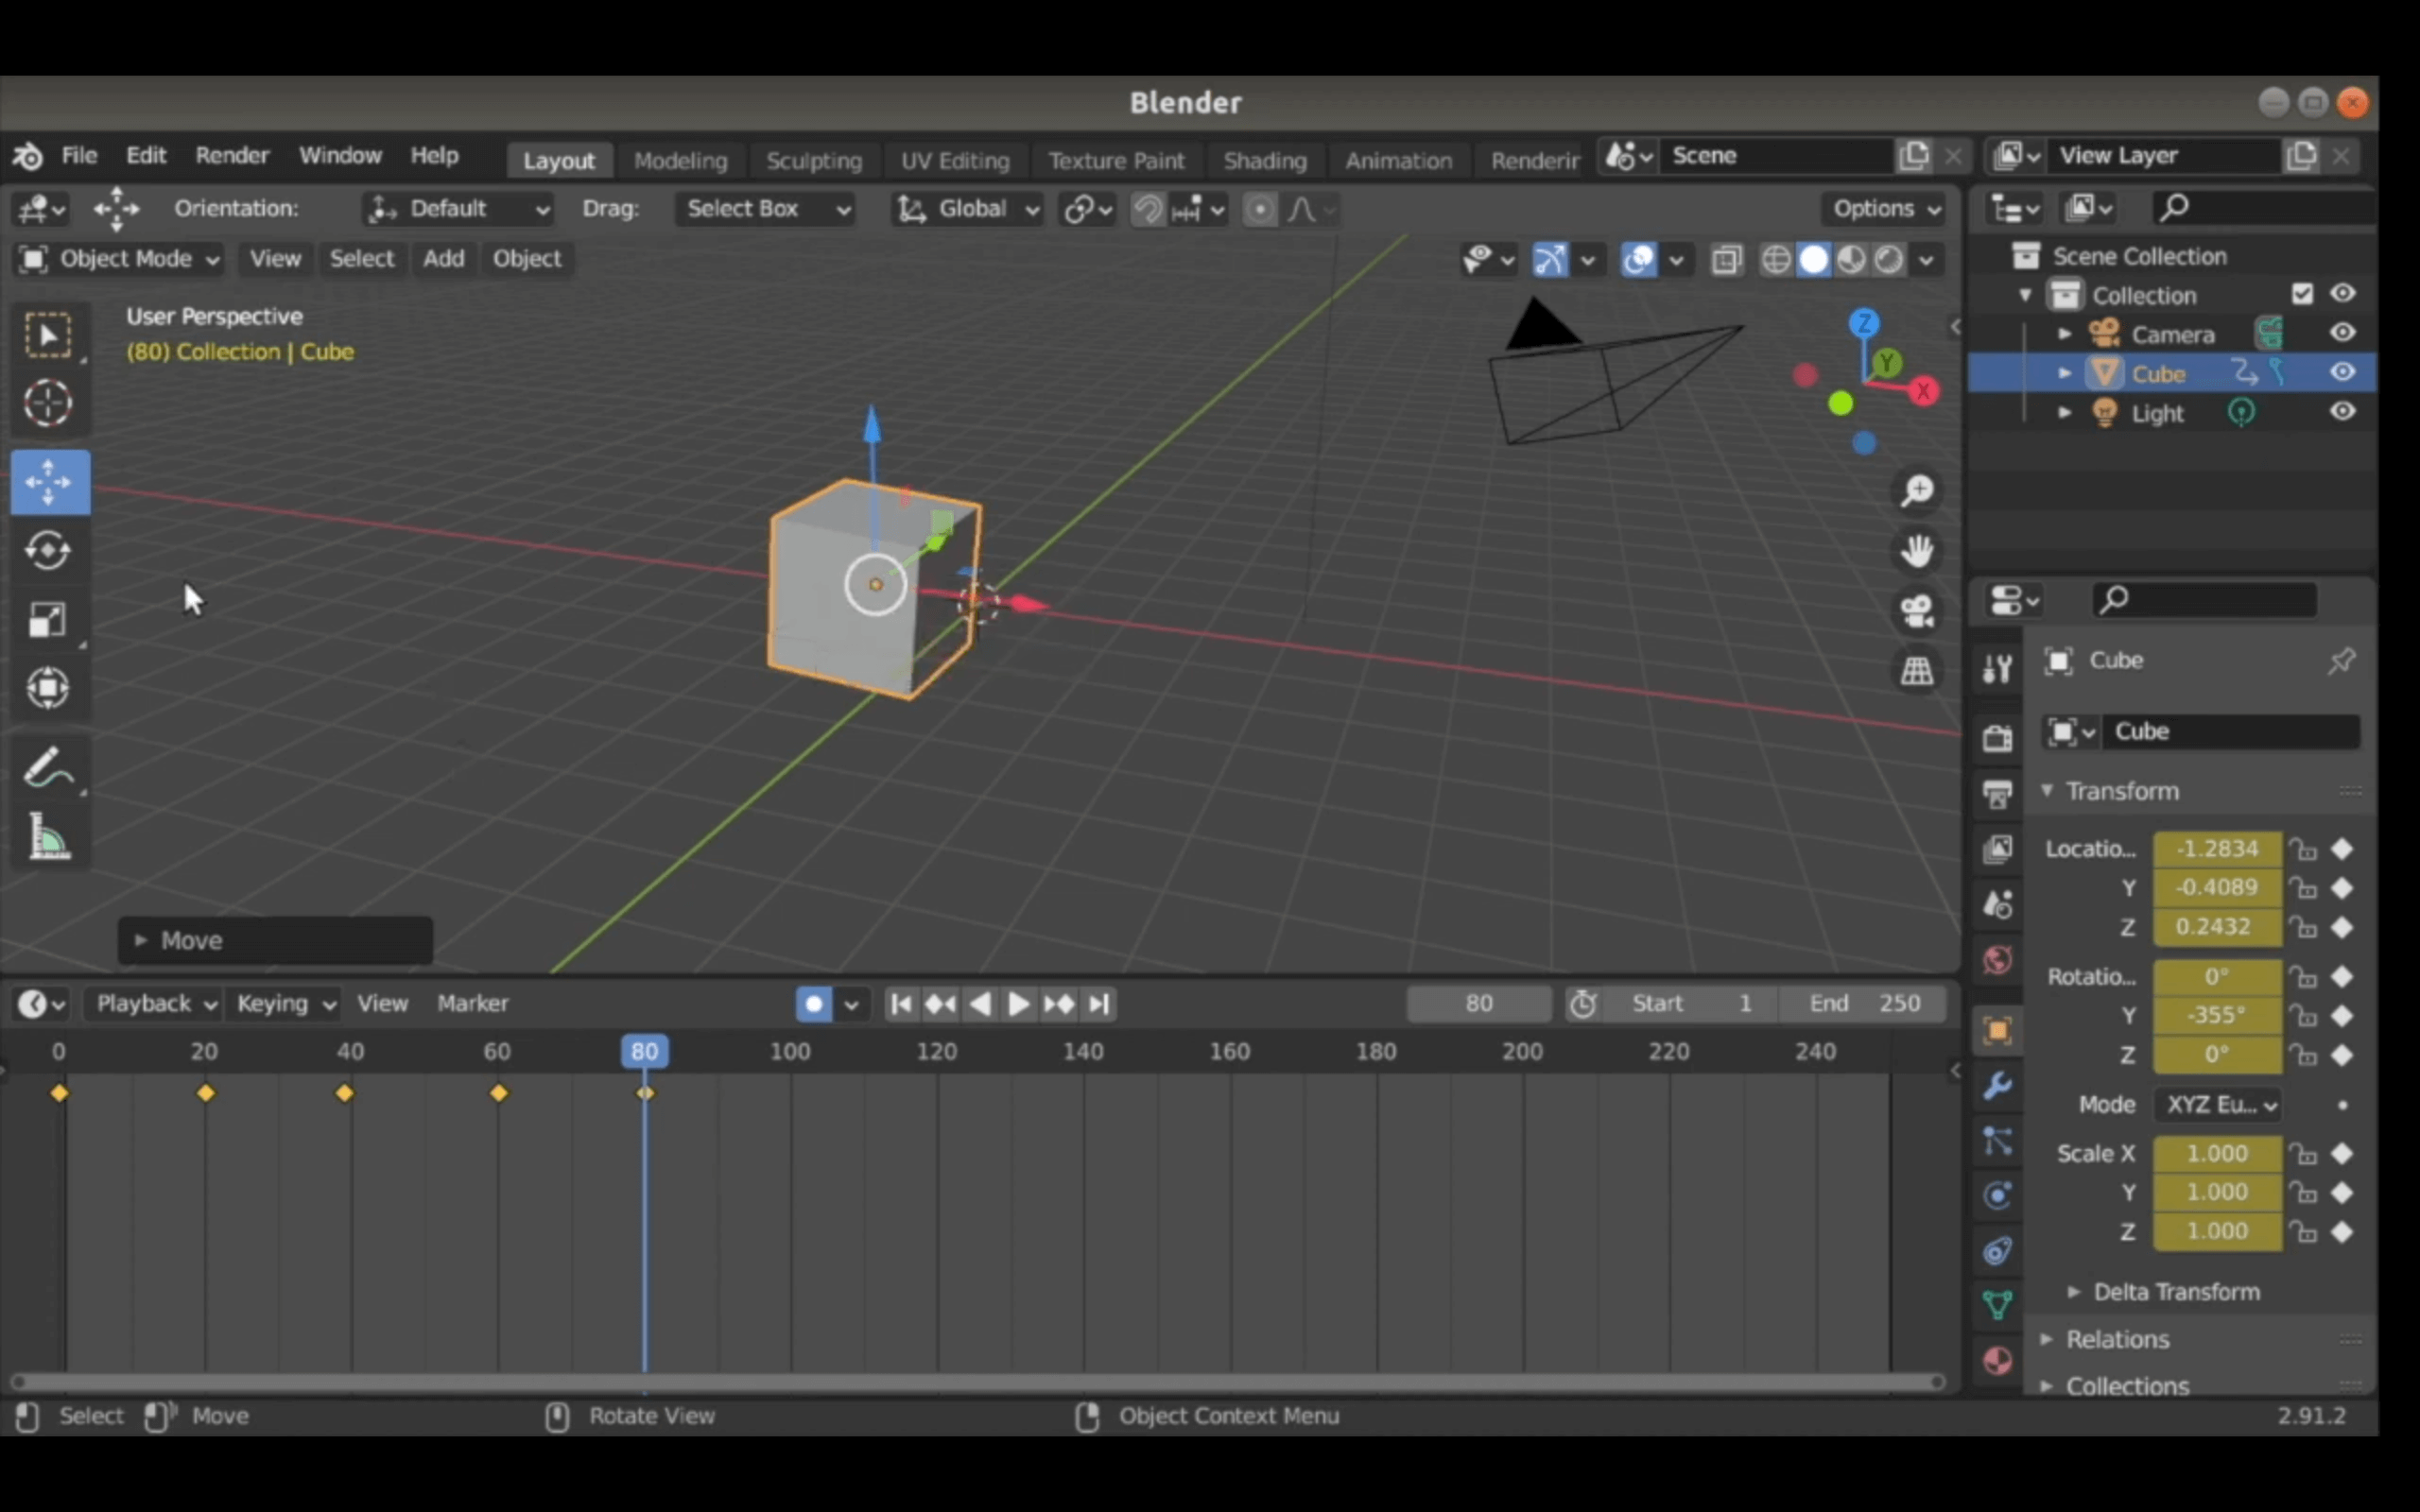
\includegraphics[width=0.7\textwidth, height=0.4\textwidth]{chapters/images/blender.png}
    \caption{Blender}
    \label{fig:my_label}
\end{figure}

\subsection{Plataforma Kibotics}

Kibotics es una plataforma web para docencia en robótica y programación. Esta plataforma se basa en tecnologías web como Django para la parte servidor y utiliza un simulador llamado Websim que se apoya en A-Frame para representar los escenarios de los ejercicios en el navegador del usuario.

Esta plataforma en línea ofrece contenidos educativos para facilitar el aprendizaje en programación a alumnos de primaria, secundaria y bachillerato. Ofrece cursos en lenguajes Scratch y Python. Los ejercicios están disponibles tanto para robots físicos como simulados. Destacan Mbot, Dron Tello y Pibot entre otros.
También ofrece interacción social gracias a un foro.

La simulación de robots reales permite  depurar el software al máximo antes de ejecutarlo en un robot físico y así reducir los costes, ya que no necesitas tener un robot para cada alumno y evitar  posibles daños de los robots y accidentes.

Para usar esta plataforma no es necesario instalar nada, solo tener acceso a Internet. Al ser una aplicación web tenemos la ventaja de que es multiplataforma y podemos usarla en distintos dispositivos.

Kibotics tiene la filosofía \textit{Learn by doing}, aprender haciendo. Las lecciones de teoría junto ejercicios prácticos hacen que los contenidos educativos se vayan adaptando según la complejidad de cada ejercicio. En la Figura 3.9 podemos ver algunos de los ejercicios que ofrecen.

\begin{figure}[H]
\begin{subfigure}{.5\textwidth}
  \centering
  % include first image
  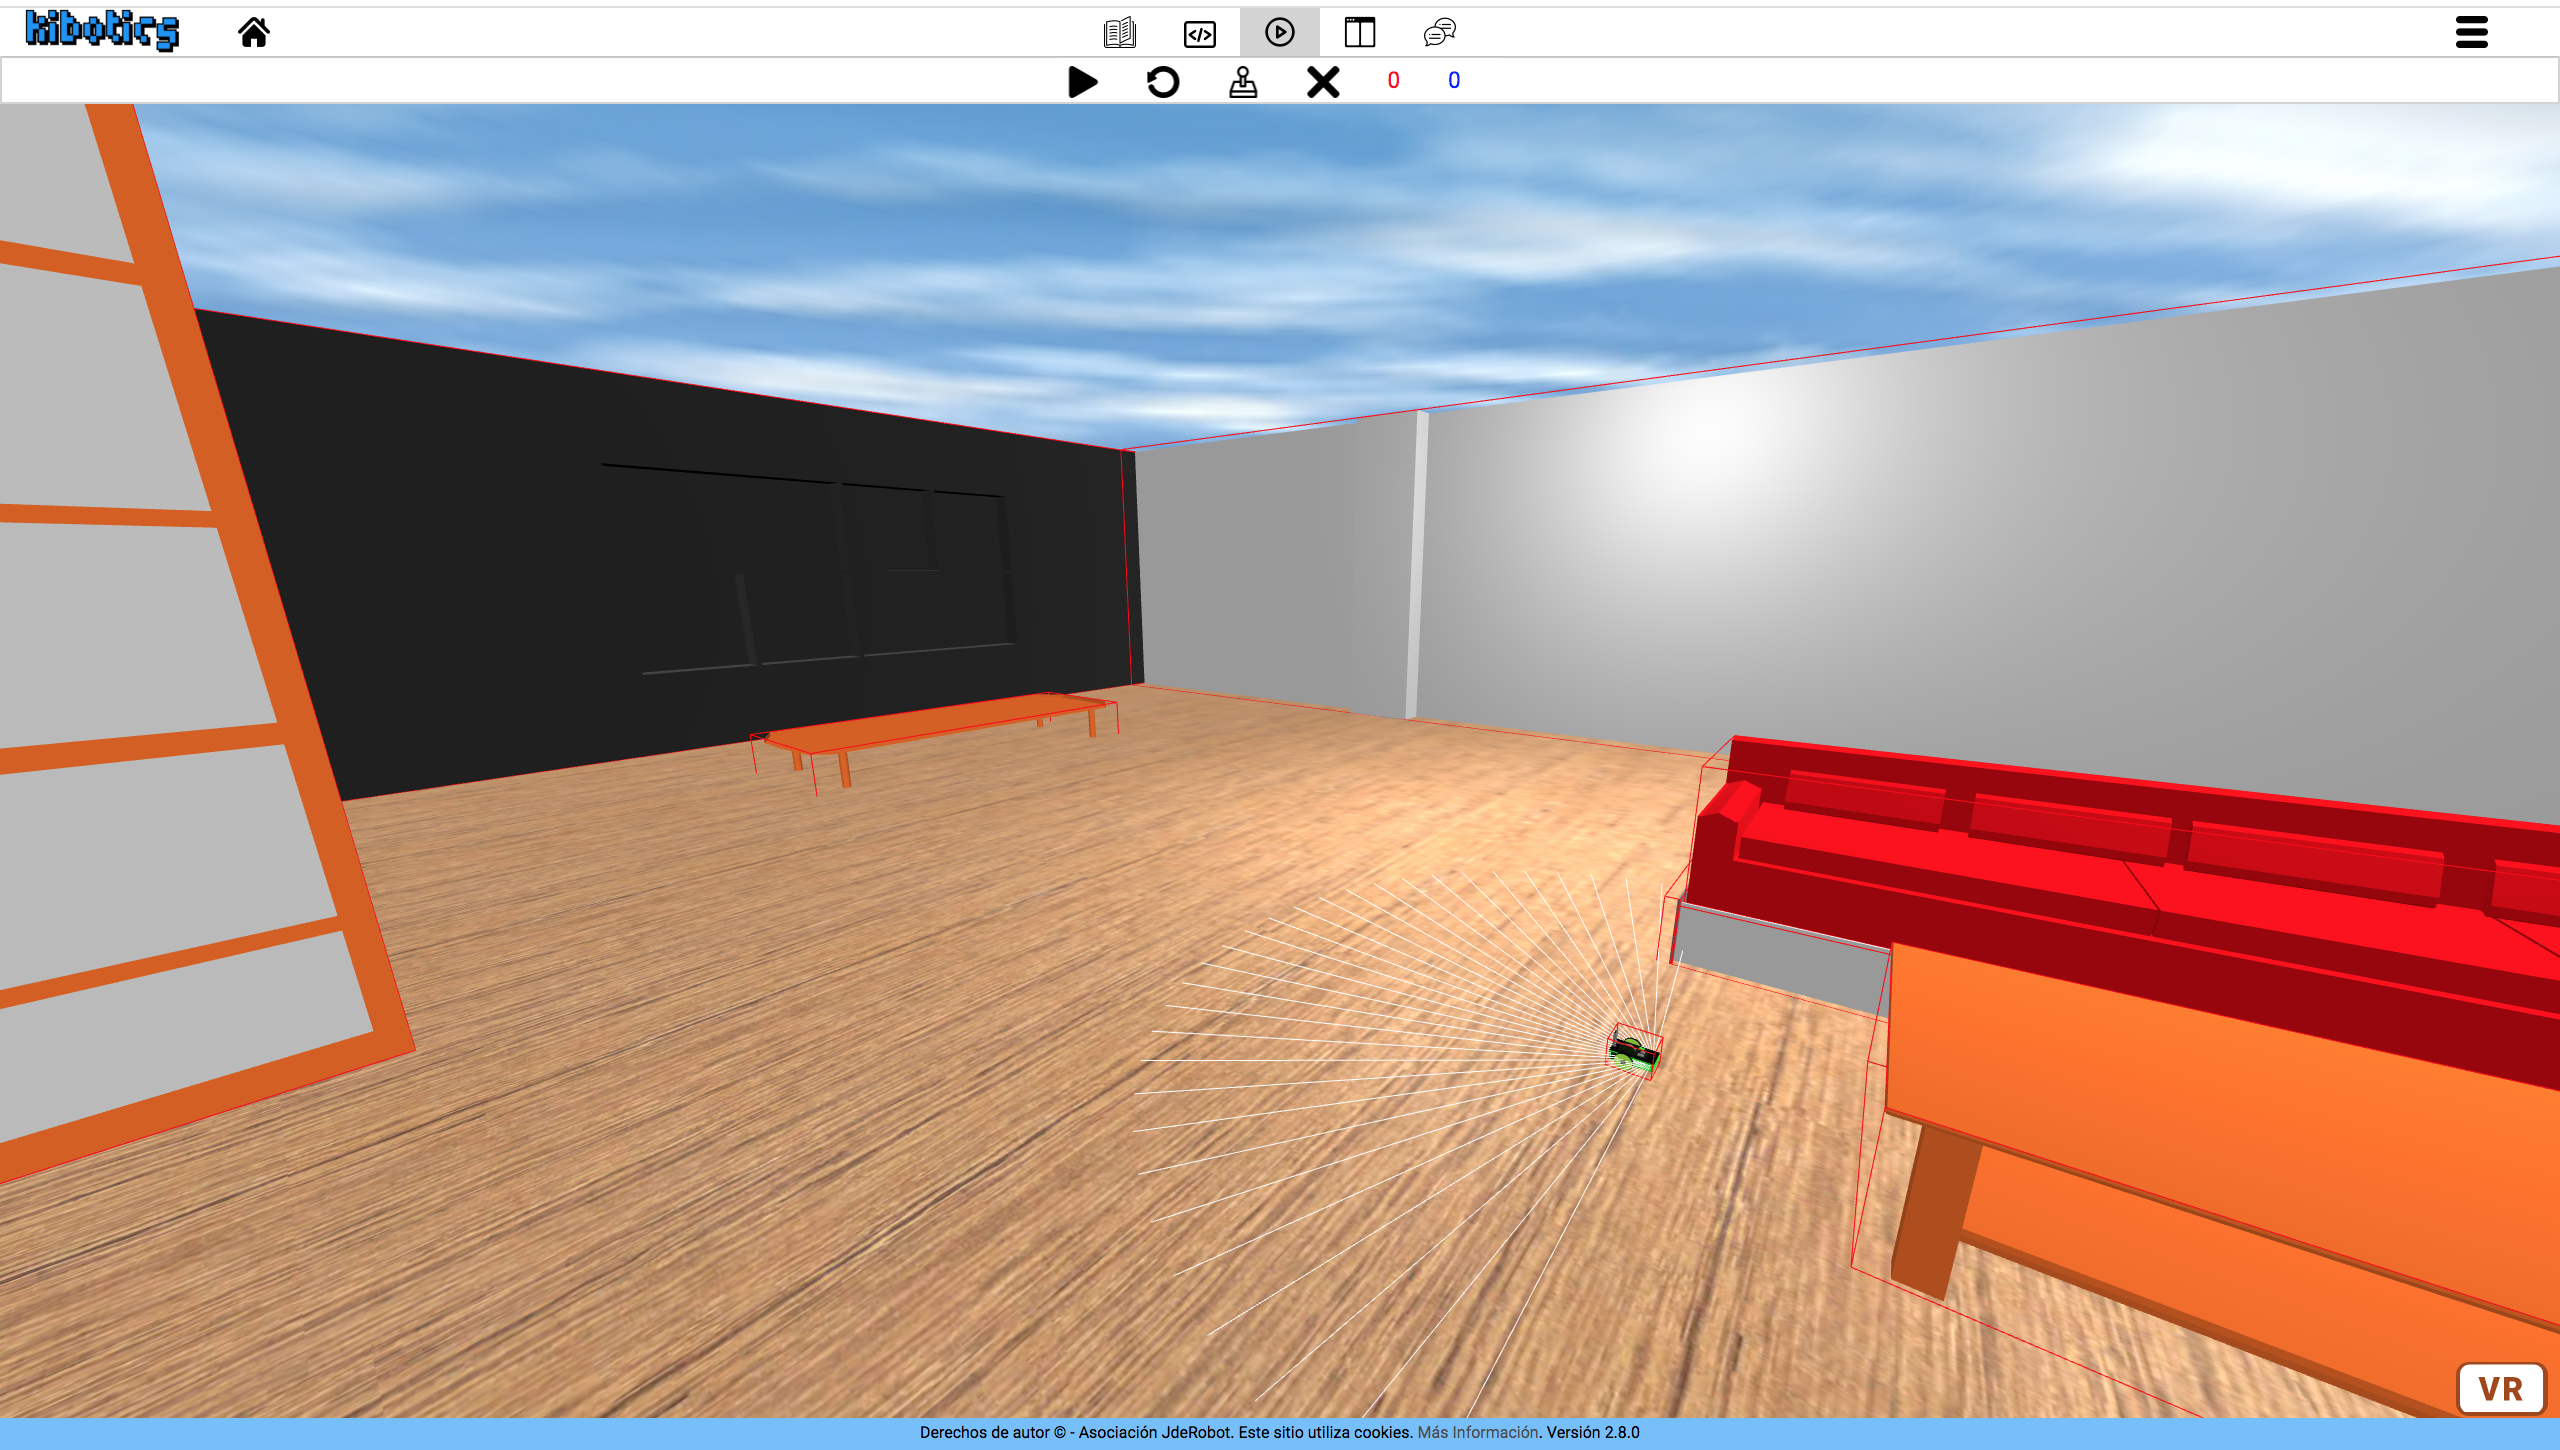
\includegraphics[width=.95\linewidth]{chapters/images/chocagira.png}  
  \caption{Choca-gira US}
  \label{fig:sub-first}
\end{subfigure}
\begin{subfigure}{.5\textwidth}
  \centering
  % include second image
  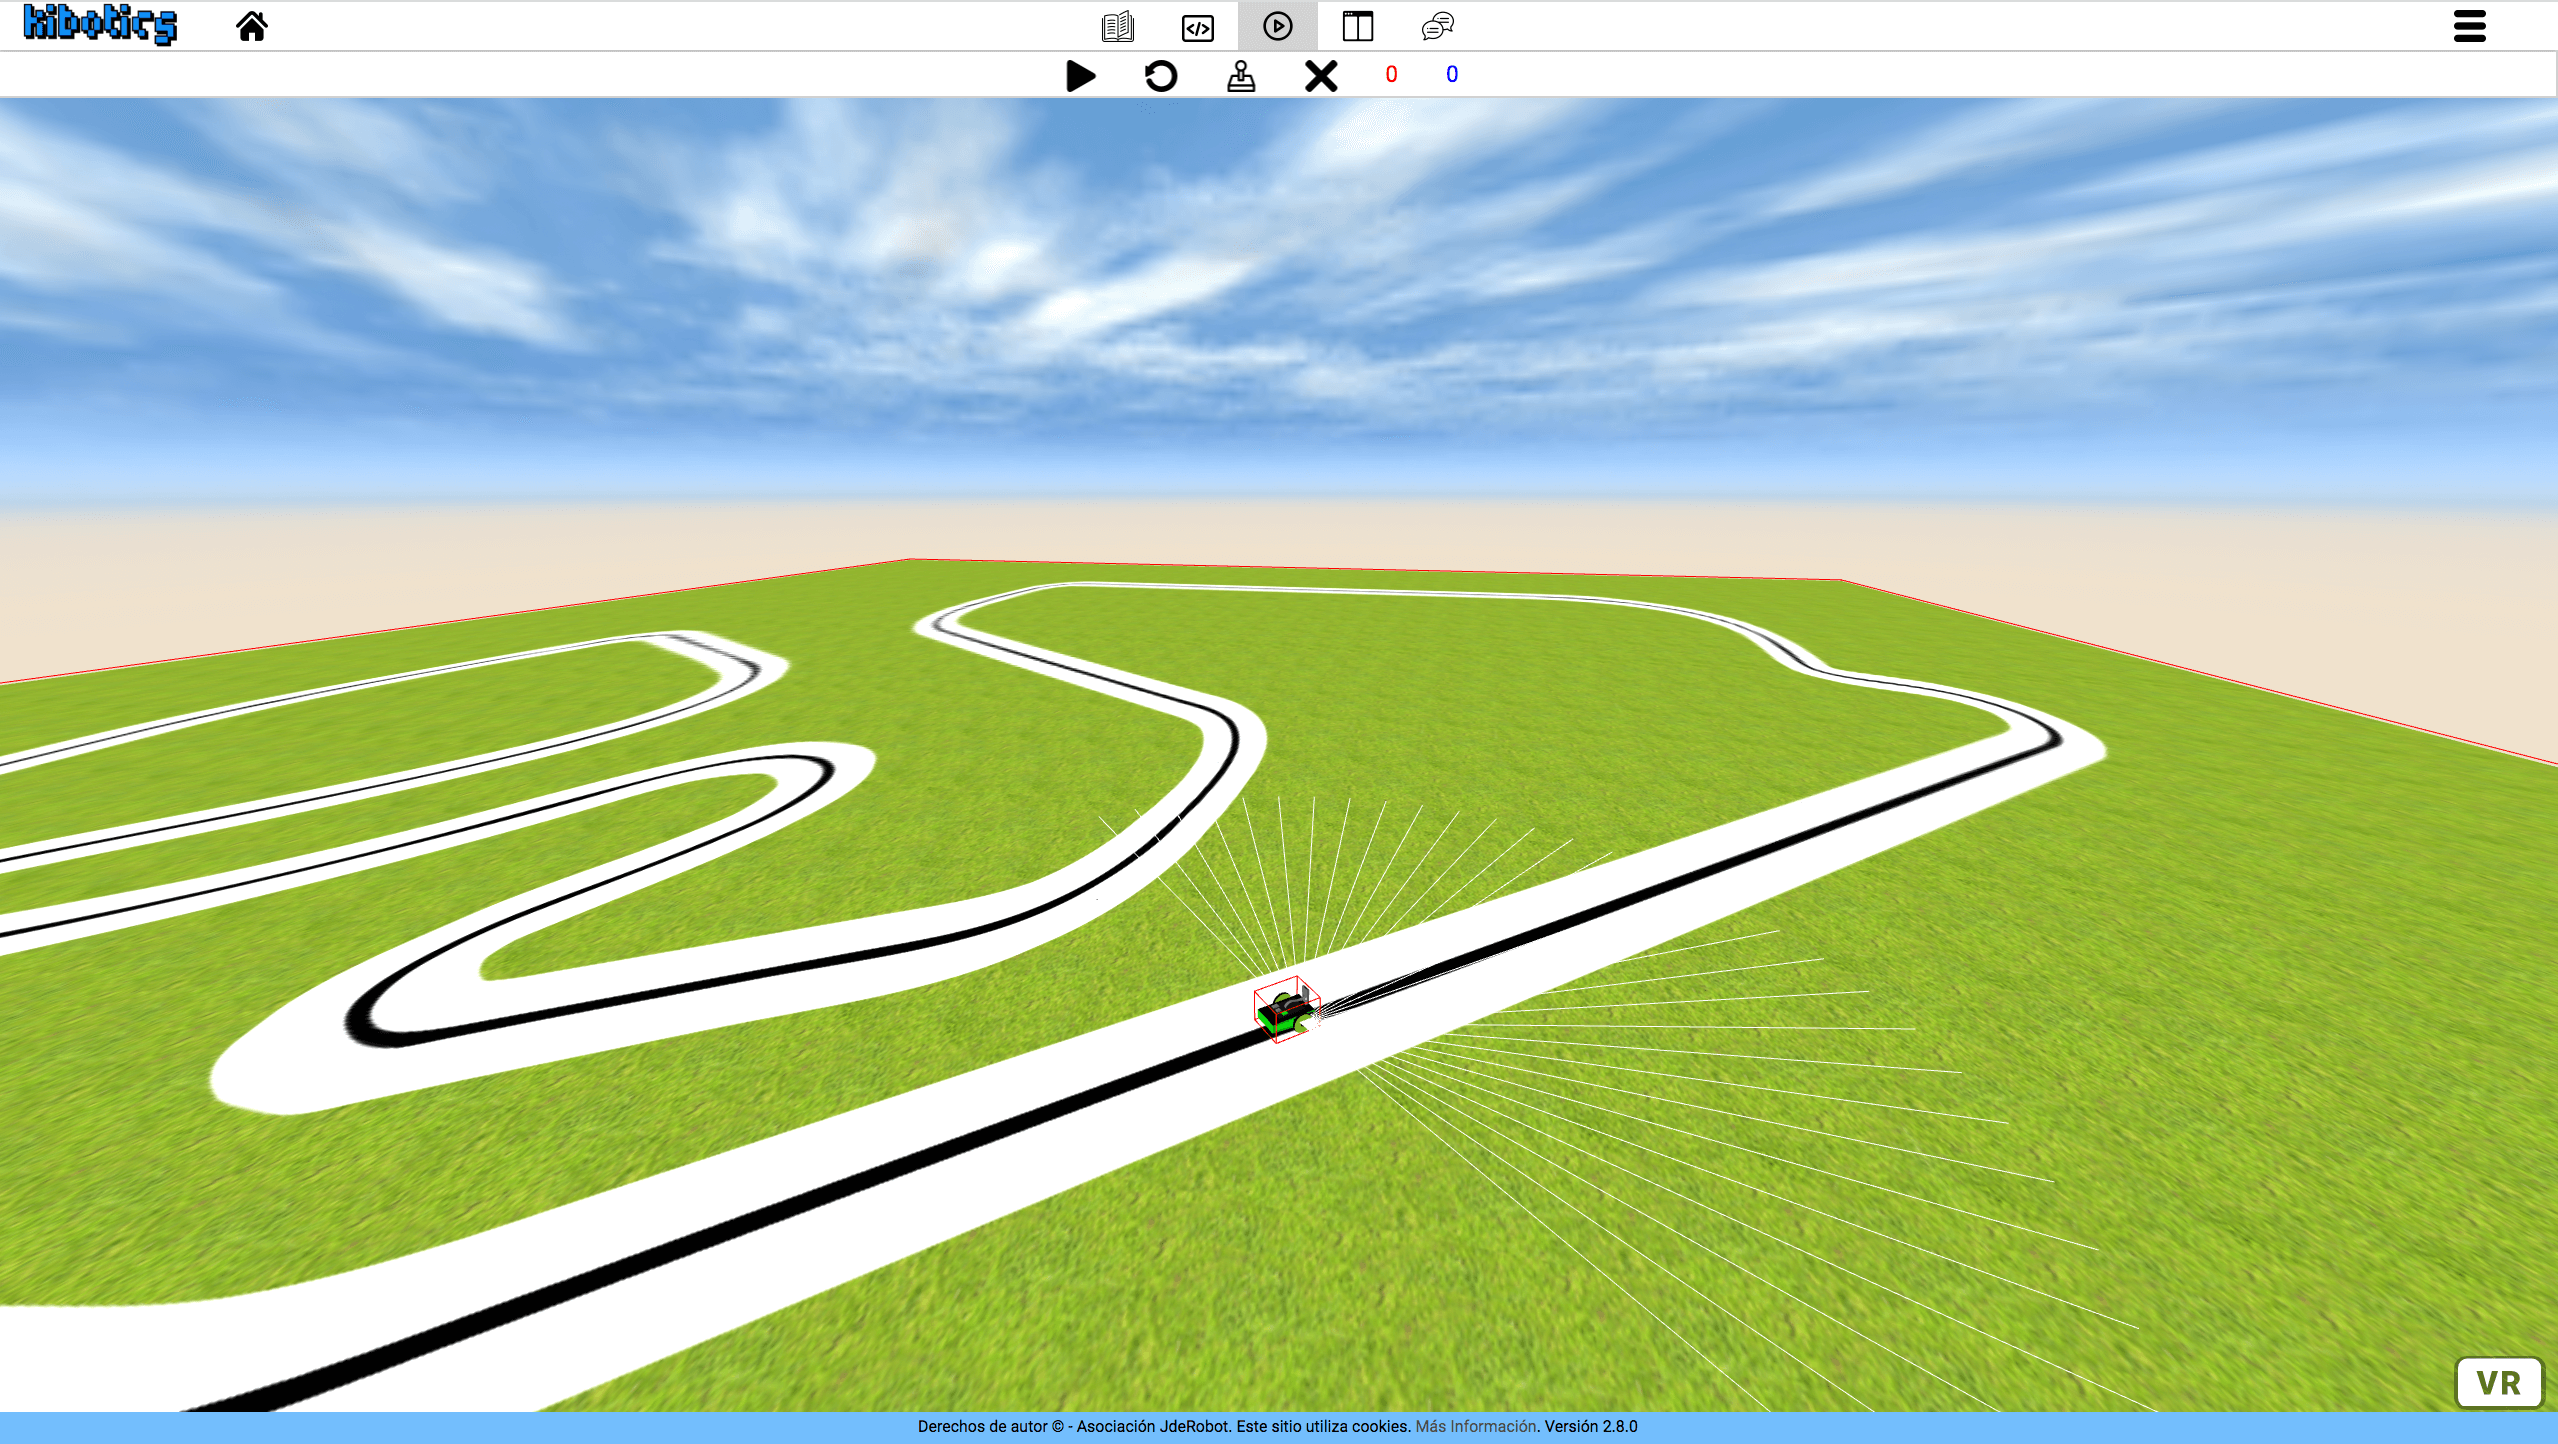
\includegraphics[width=.95\linewidth]{chapters/images/siguelineasir.png}  
  \caption{Sigue líneas IR}
  \label{fig:sub-second}
\end{subfigure}
\begin{subfigure}{.5\textwidth}
  \centering
  % include third image
  \includegraphics[width=.95\linewidth]{chapters/images/atraviesabosque.png}  
  \caption{Atraviesa Bosque}
  \label{fig:sub-third}
\end{subfigure}
\begin{subfigure}{.5\textwidth}
  \centering
  % include fourth image
  \includegraphics[width=.95\linewidth]{chapters/images/colores.png}  
  \caption{Sigue objeto con visión}
  \label{fig:sub-fourth}
\end{subfigure}
\caption{Ejercicios Kibotics}
\label{fig:partes robot}
\end{figure}


Kibotics en los últimos años ha ofrecido cursos para la escuela de pensamiento computacional INTEF, el ayuntamiento de Fuenlabrada, la empresa Logix5, Universidad Rey Juan Carlos, IES Martinez Uribarri (Salamanca) y la Comunidad de Madrid \cite{kiboticspdf}.


\subsection{Navegadores web utilizados}

En este Trabajo Fin de Grado se han usado los navegadores Chrome y Firefox por ser los navegadores más extendidos y que proporcionan gran rendimiento, estabilidad y seguridad. Se han utilizado para la visualización de la página web de Kibotics y la ejecución y pruebas de los distintos ejercicios. 



\cleardoublepage

% BIBLIOGRAFIA %
%%%%%%%%%%%%%%%%%%%%%%%%%%%%%%%%%%%%%%%%%%%%%%%%%%%%%%%%%%%%%%%%%%%%%%%%%%%%%%%%
% REFERENCES / BIBLIOGRAPHY
\cleardoublepage
\begin{thebibliography}{69}

% AUTHOR - TITLE - YEAR
\bibitem{intro}``Kibotics.” https://kibotics.org/ (accedida  Abr. 18, 2021).

\bibitem{intro1} R. Barrientos Sotelo, Víctor Ricardo; García Sánchez, José Rafael; Silva Ortigoza, ``Robots Móviles: Evolución y Estado del Arte,” Polibits, vol. 19, pp. 228–237, 2007, doi: 10.3233/978-1-60750-530-3-228.

\bibitem{davinci} ``Abex.” https://www.abexsl.es/es/sistema-robotico-da-vinci/que-es (accedida Abr. 18, 2021).

\bibitem{roboticakids} ``Los mejores KITS de ROBÓTICA y ROBOTS para NIÑOS por edades en 2020.” https://revistaderobots.com/robotica-educativa/comprar-kits-de-robotica-y-robots-programables-para-ninos/ (accedida Abr. 18, 2021).

\bibitem{mbot}	``mBot Explorer Kit,Makeblock ROBOTIX.” https://www.robotix.es/es/mbot (accedida Abr. 18, 2021).

\bibitem{www}	``¿Qué es la World Wide Web (www) y cómo funciona?” https://www.fotonostra.com/digital/paginasweb.htm (accedida Abr. 18, 2021).

\bibitem{tecnologiasweb} ``Introducción a las tecnologías web · myTeachingURJC/2018-19-CSAAI Wiki.” https://github.com/myTeachingURJC/2018-19-CSAAI/wiki/Introducción-a-las-tecnologías-web\#tecnologías-en-el-lado-del-servidor (accedida Abr. 18, 2021).


\bibitem{tecnologiascliente}	``Tecnologías y herramientas para el desarrollo web.” http://cv.uoc.edu/annotation/a9c35c372dcee6e6b92afad6993cd048/620334/PID\_00250214/PID\_00250214.html (accedida Abr. 18, 2021).


\bibitem{django}``The Web framework for perfectionists with deadlines | Django.” https://www.djangoproject.com/ (accedida Abr. 18, 2021).

\bibitem{insta}	``Web Service Efficiency at Instagram with Python | by Instagram Engineering | Instagram Engineering.” https://instagram-engineering.com/web-service-efficiency-at-instagram-with-python-4976d078e366  (accedida Abr. 18, 2021).

\bibitem{node}	``Acerca | Node.js.” https://nodejs.org/es/about/ (accedida Abr. 18, 2021).

\bibitem{nodenetflix} ``Top Companies That Use Node.JS in Production: Netflix, Trello, and Co.” https://youteam.io/blog/top-companies-that-used-node-js-in-production/ (accedida Abr. 18, 2021).


\bibitem{php1}	``¿Qué es PHP? y ¿Para qué sirve? Un potente lenguaje de programación para crear páginas web. (CU00803B).” https://www.aprenderaprogramar.com/index.php?option=com\_content\&view\=article\&id=492:ique-es-php-y-ipara-que-sirve-un-potente-lenguaje-de-programacion-para-crear-paginas-web-cu00803b\&catid=70\&Itemid=193 (accedida Abr. 18, 2021).
  
\bibitem{php2}	``Top 10 websites built with PHP technology - Facebook, Yahoo...” https://cybercraftinc.com/blog/top-10-projects-developed-with-php-technology (accedida Abr. 18, 2021).


\bibitem{multimedia} ``La importancia del contenido multimedia en educación.” https://www.cursosfemxa.es/blog/14089-la-importancia-del-contenido-multimedia-en-educacion (accedida Abr. 18, 2021).


\bibitem{aprendizaje} E. Andrade \& E. Chacón, ``Implicaciones teóricas y procedimentales de la clase invertida,” Pulso, vol. 41, pp. 251–268, 2018.

\bibitem{videoeducativo} ``El Vídeo Educativo como recurso dinamizador del Aprendizaje - EVirtualplus.” https://www.evirtualplus.com/video-educativo-como-recurso-aprendizaje/ (accedida Abr. 20, 2021).

\bibitem{importanciamultimedia}	``La Importancia Del Contenido Multimedia En La Educación.” https://es.calameo.com/read/005984440640dded50f70 (accedida Abr. 18, 2021).

\bibitem{kahoot}	``Play Kahoot! - Enter game PIN here!” https://kahoot.it/ (accedida Abr. 18, 2021).

\bibitem{roboticaedu} ``Robótica educativa: ¿qué es y cuáles son sus ventajas?” https://www.unir.net/educacion/revista/robotica-educativa/ (accedida Abr. 20, 2021).

\bibitem{scratch} ``Scratch - Imagine, Program, Share.” https://scratch.mit.edu/ (accedida Abr. 18, 2021).

\bibitem{openroberta} 	E. P. Morales \& M. F. G. Muñoz, ``Manual Open Roberta.” http://robomatrix.org/wp-content/uploads/2021/Manual\_OpenRoberta.pdf (accedida May 09, 2021).

\bibitem{ev3} ``LEGO MINDSTORMS Education EV3 | LEGO® Education.” https://www.robotix.es/es/lego-mindstorms-education-ev3 (accedida May 09, 2021).
\bibitem{legoeducation} ``Recursos, Software y Actividades GRATIS | LEGO Education - ROBOTIX.” https://www.robotix.es/es/descargar-software-lego-education (accedida May 09, 2021)
\bibitem{mblock} ``What Is mBlock 5?” https://www.yuque.com/makeblock-help-center-en/mblock-5/overview (accedida May 09, 2021).


\bibitem{competiciones}	``Competiciones de robótica educativa a los que apuntarse.” https://blog.juguetronica.com/competiciones-de-robotica-educativa/\#robocampeones (accedida Abr. 18, 2021).

\bibitem{robocup} ``RoboCupJunior – Creating a learning environment for today, fostering technological advancement for tomorrow.” https://junior.robocup.org/ (accedida Abr. 20, 2021).

\bibitem{eurobot}	``EUROBOT JR.” http://www.eurobot.es/index.php/eurobot-jr (accedida Abr. 20, 2021).
\bibitem{firstlego} ``FIRST LEGO League.” https://www.firstlegoleague.es/ (accedida Abr. 20, 2021).
\bibitem{vex} ``Vex Spain | Torneos.” https://vexspain.com/vex-iq/torneos/ (accedida Abr. 20, 2021).

\bibitem{robocampeones} ``Robocampeones”
http://robocampeones.org/(accedida Abr. 20, 2021).

\bibitem{imgs} Imágenes de:	``Pexels.” https://www.pexels.com/es-es/ (accedida Abr. 18, 2021).

\bibitem{imgs2} Imágenes de :`` Pixabay.” https://pixabay.com/es/ (accedida Abr. 18, 2021).

\bibitem{}	``Programación para niños con vídeos de Scratch y Arduino.” https://revistaderobots.com/robots-y-robotica/lenguajes-de-programacion-para-ninos-y-ninas/ (accedida Abr. 18, 2021).

\bibitem{}	``Tecnologías para el desarrollo web más actuales | proun Madrid - Asturias.” https://www.proun.es/blog/tecnologias-web-actuales/ (accedida Abr. 18, 2021).
\bibitem{}	``Conceptos básicos sobre tecnologías de desarrollo web - ingeniovirtual.com.” https://www.ingeniovirtual.com/conceptos-basicos-sobre-tecnologias-de-desarrollo-web/ (accedida Abr. 18, 2021).
\bibitem{} ``Competencia docente de la robótica educativa: ¿una realidad o un nuevo reto para el profesorado? - Equipamiento para centros educativos.” https://www.interempresas.net/Tecnologia-aulas/Articulos/156527-Competencia-docente-de-robotica-educativa-realidad-o-nuevo-reto-para-profesorado.html (accedida Abr. 18, 2021).



\bibitem{}	``Así se enseña robótica y programación en las aulas españolas.” https://www.educaciontrespuntocero.com/noticias/robotica-y-programacion-espana/ (accedida Abr. 18, 2021).

\bibitem{robotica} ``Historia de robotica - el mundo de la robotica 604.” https://sites.google.com/site/elmundodelarobotica604/historia-de-robotica (accedida Abr. 18, 2021).

\bibitem{modeloiter} ``Modelos de desarrollo de software” https://www.elconspirador.com/2013/08/19/modelos-de-desarrollo-de-software/ (accedida Abr. 25, 2021).

\bibitem{javascript} J. Eguíluz Pérez, “Introducción a JavaScript.”www.librosweb.es ( accedida Abr. 26, 2021)


\bibitem{html}	``HTML: lenguaje de marcado de hipertexto | MDN.” https://developer.mozilla.org/en-US/docs/Web/HTML (accedida May 02, 2021).

\bibitem{html2} ``Qué es HTML5: Definición y funcionamiento | OpenWebinars." https://openwebinars.net/blog/que-es-html5/ (accedida May 02, 2021).


\bibitem{python} R. G. Duque, ``Python PARA TODOS.” http://mundogeek.net/tutorial-python/ (accedida May 03, 2021).
\bibitem{aceeditor} ``Ace - The High Performance Code Editor for the Web.” https://ace.c9.io/ (accedida May 03, 2021).
\bibitem{blocky} ``Blockly  |  Google Developers.” https://developers.google.com/blockly (accedida May 03, 2021).


\bibitem{json} ``Trabajando con JSON \- Aprende sobre desarrollo web | MDN.” https://developer.mozilla.org/es/docs/Learn/JavaScript/Objects/JSON (accedida May 03, 2021).
\bibitem{json2} ``JSON.” https://desarrolloweb.com/home/json (accedida May 03, 2021).

\bibitem{tfjs} ``TensorFlow Core | Aprendizaje automático para principiantes y expertos.” https://www.tensorflow.org/overview?hl=es-419 (accedida May 03, 2021).

\bibitem{waa} ``Web Audio API - Referencia de la API Web | MDN.” https://developer.mozilla.org/es/docs/Web/API/Web\_Audio\_API (accedida May 03, 2021).
\bibitem{tm} ``Teachable Machine.” https://teachablemachine.withgoogle.com/ (accessed May 03, 2021).

\bibitem{aframe} ``Introduction – A-Frame.” https://aframe.io/docs/1.2.0/introduction/\#getting-started (accedida May 03, 2021).
\bibitem{blender}  ``blender.org - Home of the Blender project - Free and Open 3D Creation Software.” https://www.blender.org/ (accedida May 03, 2021).
\bibitem{navegador} ``Vista de Navegadores web | El Tecnológico.” https://revistas.utp.ac.pa/index.php/el-tecnologico/article/view/1287/html (accedida May 03, 2021).

\bibitem{kiboticspdf} J.M. Cañas.  ``Robótica del siglo XXI y edicación” https://gsyc.urjc.es/jmplaza/activities/charla-prosegur2020.pdf (accedida May 05, 2021 )

\bibitem{tensorflowmodel} ``Modelos de TensorFlow.js.” https://www.tensorflow.org/js/models?hl=es-419 (accedida May 28, 2021).

\end{thebibliography}


\end{document}